\documentclass[12pt,a4paper]{report}
\usepackage[utf8]{inputenc}
\usepackage[english,greek]{babel}
\usepackage{alphabeta}
\usepackage{subfiles}
\usepackage[document]{ragged2e}
\usepackage{amsmath}
\usepackage{amsfonts}
\usepackage{chngcntr}
\usepackage{moresize}
\usepackage{titlesec}
\usepackage{url}
\usepackage{caption}
\usepackage{subcaption}
\usepackage{float}
\usepackage{listings}
\usepackage[toc,page]{appendix}
\usepackage{minted}

\addto\captionsenglish{%
    \renewcommand{\bibname}{\selectlanguage{greek}Bibliograf\'ia}%
}

\usepackage{graphicx}
\graphicspath{{misc/}}
\graphicspath{{fwto/}}
\graphicspath{{biosignals/}}
\graphicspath{{r01database/}}
\graphicspath{{daisy/}}

\usepackage{geometry}
 \geometry{
 a4paper,
 total={150mm,240mm},
 left=30mm,
 top=30mm,
 }

 \def\blankpage{%
      \clearpage%
      \thispagestyle{empty}%
      \addtocounter{page}{-1}%
      \null%
      \clearpage}

\counterwithin{equation}{section}
\newcommand{\gr}{\selectlanguage{greek}}
\newcommand{\en}{\selectlanguage{english}}
\newtheorem{definition}{\gr Ορισμός}[chapter]
\newtheorem{theorem}{\gr Θεώρημα}[chapter]
\newtheorem{proposition}{\gr Πρόταση}[chapter]
%%
\newcommand{\shortdoctitle}{Διπλωματική Εργασία}
\newcommand{\doctitle}{Σχεδίαση, Υλοποίηση και Αξιολόγηση Αυτόματων Μεθόδων Διαχωρισμού Βιοσημάτων}
\newcommand{\docsubtitle}{Υπότιτλος εγγράφου}
\newcommand{\division}{Τηλεπικοινωνιών και Τεχνολογίας Πληροφορίας}
\newcommand{\lab}{Εργαστήριο Ενσύρματης Τηλεπικοινωνίας}

\newcommand{\me}{Λάμπη Παπακώστα του Νικολάκη} %(σε γενική πτώση) ΠΡΟΣΟΧΗ: στοιχεία σε γενική πτώση. Παράδειγμα: Άγγελου Σικελιανού του Ιωάννη
%
\newcommand{\nomme}{Λάμπης Παπακώστας του Νικολάκη} %(σε ονομαστική πτώση) ΠΡΟΣΟΧΗ: στοιχεία σε ονομαστική πτώση. Παράδειγμα: Άγγελος Σικελιανός του Ιωάννη
%
\newcommand{\studnum}{228467}
\newcommand{\keywords}{Λέξεις Κλειδιά}
\newcommand{\monthyear}{Μάρτιος 2019}

\newcommand{\supname}{Ευάγγελος Δερματάς}
\newcommand{\suptitle}{Αναπληρωτής Καθηγητής}
\newcommand{\supuni}{Πανεπιστήμιο Πατρών}

\newcommand{\cosupname}{Συνεπιβλέποντας Καθηγητής}
\newcommand{\cosuptitle}{Τίτλος Συνεπιβλέποντα Καθηγητή}
\newcommand{\cosupuni}{Πανεπιστήμιο Συνεπιβλέποντα}

\newcommand{\headofdivision}{Θεόδωρος Αντωνακόπουλος}
\newcommand{\headofdivisiontitle}{Καθηγητής}
%%

\begin{document}

\pagenumbering{arabic}
\pagestyle{plain}

\begin{titlepage}
\begin{center}
% Upper part of the page
{\large ΠΑΝΕΠΙΣΤΗΜΙΟ ΠΑΤΡΩΝ - ΠΟΛΥΤΕΧΝΙΚΗ ΣΧΟΛΗ}\\
\large ΤΜΗΜΑ ΗΛΕΚΤΡΟΛΟΓΩΝ ΜΗΧΑΝΙΚΩΝ\\ΚΑΙ ΤΕΧΝΟΛΟΓΙΑΣ ΥΠΟΛΟΓΙΣΤΩΝ\\
\hfill \break

\includegraphics[width= 0.8\textwidth]{misc/up_landscape.jpg}\\
\hfill \break
{\Large Τομέας: \division \\
Εργαστήριο: \lab }\\[1cm]

{\emph{\Large{\shortdoctitle }}}\\ [0.5cm]
του φοιτητή του Τμήματος Ηλεκτρολόγων Μηχανικών και Τεχνολογίας\\
Υπολογιστών της Πολυτεχνικής Σχολής  του Πανεπιστημίου Πατρών\\[1cm]

{\Large Παπακώστα Λάμπη του Νικολάκη}\\[0.5cm]
{\large Αριθμός μητρώου: 228467}\\[1cm]

\emph{\large Θέμα}\\[0.5cm]
\textbf{\large Σχεδίαση, Υλοποίηση και Αξιολόγηση Αυτόματων Μεθόδων Διαχωρισμού Βιοσημάτων }\\[1cm]
\emph{\large Επιβλέπων}\\[0.5cm]
\large \suptitle \, \supname, \supuni \\[1cm]
\large{Αριθμός Διπλωματικής Εργασίας: 228467/2019 }\hspace{3cm}
\vfill
% Bottom of the page
\large{Πάτρα, Μάρτιος, 2019 }
\end{center}
\end{titlepage}

\blankpage
\pagestyle{empty}
\begin{center}
{\LARGE ΠΙΣΤΟΠΟΙΗΣΗ\\[1cm]}
\large Πιστοποιείται ότι η διπλωματική εργασία με θέμα\\[1cm]
\textbf{\large \doctitle }\\[1cm]
του φοιτητή του Τμήματος Ηλεκτρολόγων Μηχανικών και Τεχνολογίας Υπολογιστών\\[1.5cm]
\me \\[0.5cm]
(Α.Μ.: \studnum )\\[1.5cm]
παρουσιάστηκε δημόσια και εξετάστηκε στο τμήμα  Ηλεκτρολόγων Μηχανικών και Τεχνολογίας Υπολογιστών στις\\[1cm]
\Large{08/03/2019}\\[1.5cm]
\end{center}
\begin{minipage}{0.5\textwidth}
\begin{flushleft} \large
Ο Επιβλέπων\\[4cm]
\supname \\
\emph{\suptitle}
\end{flushleft}
\end{minipage}
\begin{minipage}{0.5\textwidth}
\begin{flushright} \large
Ο Διευθυντής του Τομέα\\[4cm]
\headofdivision\\
\emph{\headofdivisiontitle}
\end{flushright}
\end{minipage}

\blankpage
\pagestyle{empty}
\hspace{10pt}
\begin{center}
\Large{Στοιχεία διπλωματικής εργασίας}\\[1cm]
{\large Θέμα:}
\textbf{\large \doctitle}\\[1cm]
\large {Φοιτητής: \textbf{\nomme}}\\[1cm]
\large{Επιβλέπων}\\
\textbf{\suptitle \, \supname , \supuni}\\[1cm]

\end{center}

\vspace{5em}



\blankpage
\pagestyle{plain}
\begin{center}
{\LARGE Περίληψη}\\[1cm]
\end{center}
Η παρούσα διπλωματική εργασία έχει ως αντικείμενο την εξέταση και την σύγκριση μεθόδων για την εξαγωγή συνιστωσών από γραμμικούς συνδυασμούς σημάτων, βασισμένο στο \en BSS \gr μοντέλο, που αφορούν το δυναμικό που παράγει η καρδιά.
\\
Παρουσιάζονται και υλοποιούνται με χρήση της \en Python \gr οι αλγόριθμοι \en FastICA \gr με κριτήριο την αρνητική εντροπία και π\en CA \gr με κριτήριο την περιοδικότητα των επιμέρους σημάτων.
\\
Τέλος, οι παραπάνω αλγόριθμοι εφαρμόζονται και συγκρίνονται σε τεχνητά περιοδικά σήματα αλλά στις βάσεις δεδομένων \en abdfecgdb \gr του \en Physionet \gr και \en DaISy \gr που περιέχουν ηλεκτροκαρδιογραφήματα από κυοφορούσες γυναίκες, χρησιμοποιώντας αντίστοιχα κριτήρια ως προς την εγγύτητα.

\blankpage

\pagestyle{plain}
\begin{center}
\en
{\LARGE Abstract}\\[1cm]
\end{center}
\en
The present diploma thesis examines and compares methods about extraction of components of linear mixed signals, based on BSS model, that refer to the voltage that heart produces.
\\
The algorithms that presented and implemented in Python are FastICA with negentropy criterion and \gr π\en CA with periodity of each component as criterion.
\\
Finally, the above methods are applied in synthesized periodic signals as well as abdfecgd database from Physionet and DaISy database, and compared with the use of proper criteria for their correctness.




\blankpage
\begin{center}
{\LARGE Ευχαριστίες}\\[1cm]
\end{center}
Θα ήθελα να ευχαριστήσω τον Αναπληρωτή Καθηγητή του Πανεπιστημίου Πατρών και επιβλέποντα της διπλωματικής μου εργασίας, Ευάγγελο Δερματά, για την άριστη συνεργασία μας, καθώς ήταν πάντοτε διαθέσιμος για βοήθεια.
\\[0.5 \baselineskip]
Επιπλέον, θα ήθελα να εκφράσω ένα μεγάλο ευχαριστώ στην οικογένεια μου για την καθημερινή οικονομική και ψυχολογική στήριξη που μου παρείχαν κατά την διάρκεια της ακαδημαϊκής μου πορείας, καθώς χωρίς αυτούς δεν θα τα κατάφερνα.

\blankpage
\gr 
\tableofcontents
\listoffigures

\chapter{\textbf{Βασικές Έννοιες}} \label{ch:ch1}
\section{Γραμμική Άλγεβρα} \label{sec:1.1}
\justifying
Σε αυτή την ενότητα θα παρουσιάσουμε μερικούς ορισμούς και θεωρήματα \cite{Strang:1},\cite{Meyer:2} από την Γραμμική Άλγεβρα, που θα μας βοηθήσουν στην κατανόηση και την ανάλυση των μεθόδων που θα χρησιμοποιήσουμε παρακάτω.
\begin{definition} \label{def:1.1}
Ένας τετραγωνικός πίνακας \en $\mathbf{A} \in \mathbb{R}^{n \times n}$ \gr ονομάζεται \emph{συμμετρικός} όταν \en $\mathbf{A} = \mathbf{A}^T$.
\end{definition}
\gr
\begin{theorem} \label{th:1.1}
Ένας συμμετρικός πίνακας έχει πάντα πραγματικές ιδιοτιμές.
\end{theorem}
\begin{theorem} \label{th:1.2}
Ένας συμμετρικός πίνακας έχει πάντα \en $n$ \gr γραμμικώς ανεξάρτητα ιδιοδιανύσματα, άρα μπορεί να διαγωνοποιηθεί. 
\end{theorem}
\begin{theorem} \label{th:1.3}
Τα ιδιοδιανύσματα ενός συμμετρικού πίνακα είναι δυνατόν να επιλεγούν κάθετα μεταξύ τους. 
\end{theorem}
\begin{definition} \label{def:1.2}
Ένας συμμετρικός πίνακας \en $\mathbf{A}\in \mathbf{R}^{n \times n}$ \gr ονομάζεται \emph{ορθογώνιος} όταν \en $\mathbf{A} \mathbf{A}^T = \mathbb{I}$ \gr και \en $\mathbf{A}^T = \mathbf{A}^{-1}$.
\end{definition}
\begin{definition} \label{def:1.3}
Τα διανύσματα \en $q_1, \ldots, q_k$ \gr είναι \emph{ορθοκανονικά} όταν: \en
    \begin{align*}
        q_i^T q_j = \begin{cases}
        & 0 \quad \text{\gr όταν \en} i \neq j, \text{\gr που δίνει την ορθογωνιότητα \en} \\
        & 1 \quad  \text{\gr όταν \en} i = j, \text{\gr που δίνει την κανονικότητα \en}
        \end{cases}
    \end{align*}
\end{definition}
\gr
\begin{theorem} \label{th:1.4} 
Έστω ένας πίνακας \en $\mathbf{A} \in \mathbb{R}^{n\times n}$, \gr με ιδιοτιμές \en $\lambda_1, \lambda_2, \ldots, \lambda_n$ \gr και \en $v_1, v_2, \ldots, v_n $ \gr τα αντίστοιχα ιδιοδιανύσματα. 'Εαν \en$\mathbf{V}$ \gr ο πίνακας που περιέχει ως στήλες τα ιδιοδιανύσματα του πίνακα \en $ \mathbf{A}$ \gr και \en $\mathbf{D} = diag(\lambda_1, \lambda_2, \ldots, \lambda_n) $ \gr ο διαγώνιος πίνακας των ιδιοτιμών κατα αντιστοιχία, τότε ο πίνακας \en $\mathbf{A}$ \gr μπορεί να γραφεί ως:\en
\begin{align*}
    \mathbf{A} = \mathbf{V} \mathbf{D} \mathbf{V}^{-1}
\end{align*}
\end{theorem}
\gr
\begin{proposition}\label{prop:1.1}
Εάν ο πίνακας \en $\mathbf{A}$ \gr είναι συμμετρικός, σύμφωνα με το Θεώρημα \ref{th:1.3}, τότε ο πίνακας \en $\mathbf{V}$ \gr είναι ορθογώνιος. Άρα ο πίνακας \en $\mathbf{A}$ \gr μπορεί να γραφεί:
\begin{align*}
    \mathbf{A} = \mathbf{V} \mathbf{D} \mathbf{V}^T
\end{align*}
\end{proposition}
\begin{definition}\label{def:1.4}
Ένας συμμετρικός πίνακας \en $\mathbf{A} \in \mathbb{R}^{n \times n}$\gr ονομάζεται \emph{θετικά ορισμένος} όταν όλες οι ιδιοτιμές του είναι θετικές.
\end{definition}
\begin{definition} \label{def:1.5}
Ένας συμμετρικός πίνακας \en $\mathbf{A} \in \mathbb{R}^{n \times n}$\gr ονομάζεται \emph{θετικά ημι-ορισμένος} όταν όλες οι ιδιοτιμές του είναι μη αρνητικές.
\end{definition}
\begin{theorem} \label{th:1.5} [Κριτήριο \en Sylvester]
\gr Αναγκαία και ικανή συνθήκη για να είναι ένας τετραγωνικός πίνακας \en $\mathbf{A}$ \gr θετικά ορισμένος εάν για τις ακόλουθες διαδοχικές ορίζουσες ισχύει ότι: \en
\begin{align*}
    D_{1} = \alpha_{11} > 0, 
    D_{2} = \begin{vmatrix}
    \alpha_{11} & \alpha_{12} \\
    \alpha_{21} & \alpha_{22}
    \end{vmatrix} > 0 , 
    D_{3} = \begin{vmatrix}
    \alpha_{11} & \alpha_{12} & \alpha_{13} \\
    \alpha_{21} & \alpha_{22} & \alpha_{23} \\
    \alpha_{31} & \alpha_{32} & \alpha_{33}
    \end{vmatrix} > 0, \ldots, D_{n} = |\mathbf{A}| > 0 
\end{align*}
\gr Αντίστοιχα, για να είναι θετικά ημι-ορισμένος θα πρέπει οι ακόλουθες διαδοχικές ορίζουσες να είναι μεγαλύτερες ή ίσες του μηδενός. 
\end{theorem}
\begin{definition} \label{def:1.6}
Μια τιμή \en $\lambda \in \mathbb{R}$ \gr και ένα διάνυσμα \en $x \in \mathbb{R}^{n \times 1}$ \gr ονομάζεται \emph{γενικευμένη ιδιοτιμή} και \emph{γενικευμένο ιδιοδιάνυσμα} ενός ζεύγους τετραγωνικών πινάκων \en ($\mathbf{A},\mathbf{B}) \quad \mathbf{A},\mathbf{B} \in \mathbf{R}^{n \times n}$ \gr, όπου ικανοποιούν την σχέση \en $\mathbf{A}x = \lambda \mathbf{B} x$. Το αντίστοιχο πρόβλημα εύρεσης των παραπάνω ποσοτήτων ονομάζεται \emph{Πρόβλημα Γενικευμένων Ιδιοτιμών} \en (General Eigenvalue Problem). \gr
\end{definition}
\begin{definition} \label{def:1.7}
Το γενικευμένο κλάσμα \en Rayleigh \gr ενός ζεύγους τετραγωνικών πινάκων \en ($\mathbf{A},\mathbf{B}$) ορίζεται: \en
\begin{align*}
    \mathbf{R} \left( \mathbf{A},\mathbf{B},w \right) = \frac{x^T \mathbf{A} x}{ x^T \mathbf{B} x}
\end{align*}
\end{definition}
\gr
\begin{theorem}\label{th:1.6} [Aρχή \en Rayleigh-Ritz]
Έστω \en $\lambda_1 \geq \lambda_2 \geq \ldots \geq \lambda_n$ \gr οι γενικευμένες ιδιοτιμές του ζεύγους \en ($\mathbf{A},\mathbf{B}$) \gr και \en $v_1, v_2, \ldots, v_n$ \gr τα αντίστοιχα γενικευμένα ιδιοδιανύσματα. Τότε ισχύει:\en
\begin{align*}
    \min_{x} \left\{ \mathbf{R}(\mathbf{A},\mathbf{B},x) \right\} = \mathbf{R}(\mathbf{A},\mathbf{B},v_1) = \lambda_1 \\
    \max_{x} \left\{ \mathbf{R}(\mathbf{A},\mathbf{B},x) \right\} = \mathbf{R}(\mathbf{A},\mathbf{B},v_n) = \lambda_n
\end{align*}
\end{theorem}
\gr
\begin{proposition} \label{prop:1.2}
Έστω ένας αντιστρέψιμος πίνακας \en $\mathbf{Q} \in \mathbf{R}^{n \times n}$,\gr όπου \en $\mathbf{A} \in \mathbb{R}^{n \times n}$ \gr ένας συμμετρικός πίνακας και \en $\mathbf{B} \in \mathbb{R}^{n \times n}$\gr ένας θετικά ορισμένος πίνακας. Τότε: \en
\begin{align*}
    \mathbf{R} (\mathbf{Q}^T \mathbf{A} \mathbf{Q},\mathbf{Q}^T \mathbf{B} \mathbf{Q},x) = \mathbf{R} (\mathbf{A},\mathbf{B},\mathbf{Q}x)
\end{align*}
\end{proposition}
\gr
\begin{proposition} \label{prop:1.3}
Όταν πολλαπλασιάζουμε το ζεύγος πινάκων με τους αριθμούς \en $a,b \in \mathbb{R}$ \gr αντίστοιχα, τότε το κλάσμα \en Rayleigh \gr γίνεται: \en
\begin{align*}
   \mathbf{R}(a\mathbf{A},b\mathbf{B},x) = \frac{a}{b}  \mathbf{R}(\mathbf{A},\mathbf{B},x)
\end{align*}
\end{proposition}
\section{Πιθανότητες και Τυχαία Σήματα} \label{sec:1.2}
\justifying
Παραθέτουμε τους ακόλουθους ορισμούς \cite{prob:15} ώστε να κάνουμε καλύτερη την κατανόηση των μεθόδων. Για τους ορισμούς, υποθέτουμε τυχαία μεταβλητή \en $x$ \gr με συνάρτηση κατανομής \en $F_x(x_i) = P\{x \leq x_i \}$ \gr και συνάρτηση πυκνότητας πιθανότητας \en $f_x(x) = \frac{\mathrm{d} F_x }{\mathrm{d} x} $ \gr.
\begin{definition} \label{def:1.8}
Η \emph{μέση τιμή} ή \emph{αναμενόμενη τιμή} μιας οποιαδήποτε συνάρτησης \en $g(x)$ \gr της τυχαίας μεταβλητής \en $x$ \gr είναι:
\begin{align*}
    E\{g(x)\} = \int\limits_{-\infty}^{\infty} g(x)f_x(x) \mathrm{d}x
\end{align*}
\end{definition}
\begin{proposition} \label{prop:1.4}
Εάν \en $a,b \in \mathbf{R}$ \gr, τότε: $E\{ax+b\} = aE\{x\}+b$
\end{proposition}
Στην πράξη όμως, επειδή δεν γνωρίζουμε την συνάρτηση πυκνότητας πιθανότητας της \en $x$, \gr υπολογίζουμε τον αντίστοιχο \emph{δειγματικό μέσο όρο}: \en
\begin{align*}
    E \{ g(x) \} = \frac{1}{m} \sum\limits_{i=1}^{m} g(x_i)
\end{align*} \gr
όπου \en $m$ \gr οι παρατηρήσεις της μεταβλητής \en $x$. \gr
\begin{definition} \label{def:1.9}
Η \emph{διασπορά} μιας τυχαίας μεταβλητής \en $x$ \gr ορίζεται ως: \en
\begin{align*}
    var(x) = E\{ (x-\mu)^2 \} = E\{x^2\} - \mu^2
\end{align*} 
όπου $μ$ η μέση τιμή της μεταβλητής \en $x$ \gr.
\end{definition}
\gr 
\begin{proposition} \label{prop:1.5}
Εάν \en $a,b \in \mathbb{R}$ \gr, τότε: $var(ax+b) = a^2 var(x)  $.
\end{proposition}
Η διασπορά αποτελεί ένα μέτρο της μεταβλητότητας μιας τυχαίας μεταβλητής ή του 'απλώματος' της κατανομής της. Με άλλα λόγια, μια κατανομή με μεγάλη διασπορά είναι 'απλωμένη', ενώ μια κατανομή με μικρή διασπορά είναι 'συγκεντρωμένη' γύρω από την μέση τιμή.
\begin{definition} \label{def:1.10}
Η τετραγωνική ρίζα της διασποράς ονομάζεται \emph{τυπική απόκλιση}. Δηλαδή: \en
\begin{align*}
    \sigma_x = \sqrt{var(x)}
\end{align*}
\end{definition}
\gr
\begin{definition} \label{def:1.11}
Μια τυχαία μεταβλητή \en $x$ \gr ονομάζεται \emph{γκαουσιανή} όταν ακολουθεί την κατανομή: \en
\begin{align*}
    f_x(x) = \frac{1}{\sigma_x \sqrt{2 \pi}} \exp \left( - \frac{(x-\mu)^2} {2 \sigma_x^2} \right )
\end{align*} \gr
και συμβολίζεται ως \en $\mathcal{N}(\mu,\sigma_x)$. \gr Μια γκαουσιανή κατονομή ονομάζεται \emph{τυπική} όταν έχει $μ = 0$ και \en $\sigma_x = 1$. \gr
\end{definition}
Επιπλέον, υποθέτουμε \en $y$ \gr τυχαία μεταβλητή που έχει από κοινού συνάρτηση κατανομής \en $F_{xy}(x_i,y_i) = P\left(x \leq x_i,y \leq y_i \right)$ \gr και από κοινού συνάρτηση πυκνότητας πιθανότητας \en $f_{xy} = \frac{\partial^2 F_{xy}}{\partial x \partial y}  $ \gr.
\begin{definition} \label{def:1.12}
Η \emph{μέση} ή \emph{αναμενόμενη} τιμή μιας οποιαδήποτε  συνάρτησης \en $g(x,y)$ \gr των τυχαίων μεταβλητών \en $x,y$ \gr ορίζεται ως: \en
\begin{align*}
    E\{g(x,y)\} = \int\limits_{-\infty}^{\infty} \int\limits_{-\infty}^{\infty} g(x,y) f_{xy}(x,y) \mathrm{d}x \mathrm{d}y
\end{align*} \gr
\end{definition}
\begin{definition} \label{def:1.13}
Η \emph{συσχέτιση} δύο τυχαίων μεταβλητών ορίζεται ως: \en
\begin{align*}
    corr(x,y)=E\{x,y\} 
\end{align*} 
\end{definition}
\gr
\begin{definition} \label{def:1.14}
Η \emph{συνδιασπορά} δύο τυχαίων μεταβλητών \en $x,y$ \gr ορίζεται ως: \en
\begin{align*}
    cov(x,y) = E\{ (x-\mu_x)(y-\mu_y)\} = corr(x,y) - \mu_x \mu_y
\end{align*}
\end{definition}
% pinakes 
\gr
\begin{definition} \label{def:1.15}
Οι τυχαίες μεταβλητές \en $x_1, x_2, \ldots, x_n$ \gr ονομάζονται \emph{στατιστικά ανεξάρτητες} όταν ισχύει:
\begin{align*}
    P(x_1,x_2,\ldots,x_n) = P(x_1) P(x_2) \ldots P(x_n)
\end{align*}
\end{definition}
Οι παραπάνω ορισμοί μπορούν να επεκταθούν και για τυχαία σήματα \cite{prob:16}. Όπως γνωρίζουμε, τα τυχαία σήματα απαρτίζονται από ακολουθίες τυχαίων μεταβλητών. Στους ακόλουθους ορισμούς θα χρησιμοποιήσουμε τους πίνακες που περιέχουν τυχαία σήματα \en $\mathbf{X}(t)$ \gr και \en $\mathbf{Y}(t)$ \gr. 
\begin{definition} \label{def:1.16}
Ο πίνακας \emph{αυτοσυσχέτισης} \en $\mathbf{R}_{XX}$ \gr ορίζεται ως: \en
\begin{align*}
    \mathbf{R}_{XX}(\tau) = E\left\{\mathbf{X}(t) \mathbf{X}^T(t+\tau) \right\}
\end{align*}
\en ενώ ο πίνακας \emph{ετεροσυσχέτισης} \en $\mathbf{R}_{XY} $ \gr ως:
\begin{align*}
    \mathbf{R}_{XY}(\tau) = E\left\{\mathbf{X}(t) \mathbf{Y}^T(t+\tau) \right\}
\end{align*}
\gr όπου $τ$ η χρονική μετατόπιση κάθε σήματος.
\end{definition}
\begin{proposition} \label{prop:1.6}
Για χρονική καθυστέρηση $τ=0$, ο πίνακας αυτοσυσχέτισης αναπαριστά την μέση τετραγωνική ισχύς του τυχαίου σήματος. Δηλαδή:
\begin{align*}
    \mathbf{R}_{XX}(0) = E\left \{ X^2(t) \right \}
\end{align*}
\end{proposition}
\begin{definition} \label{def:1.17}
Ο πίνακας \emph{συνδιασποράς} \en $\mathbf{C}_{X}$ \gr ορίζεται ως: \en
\begin{align*}
    \mathbf{C}_{X} = E\left \{ (\mathbf{X} - \mu_{X}) (\mathbf{X} - \mu_{X})^T \right \}
\end{align*}
\gr όπου \en $\mu_X$ \gr ο μέσος όρος του πίνακα \en $\mathbf{X} $. \gr
\end{definition}
\section{\en Principal Component Analysis - PCA} \label{sec:1.4}
\justifying
\gr Η κεντρική ιδέα της ανάλυσης κυρίων συνιστωσών (\en PCA)\cite{pca:3} \gr είναι να μειώσει τις διαστάσεις ενός συνόλου δεδομένων, το οποίο περιέχει ένα μεγάλο αριθμό από συσχετισμένες μεταβλητές, διατηρώντας όσο το δυνατό την ίδια πληροφορία με το αρχικό σύνολο δεδομένων. Το παραπάνω αποτέλεσμα επιτυγχάνεται με τον μετασχηματισμό των αρχικών δεδομένων σε ένα νέο σύνολο μεταβλητών, τις κύριες συνιστώσες (\en PC). \gr Οι κύριες συνιστώσες είναι μεταξύ τους ασυσχέτιστες και είναι διατεταγμένες με τέτοιο τρόπο ώστε οι πρώτες κατά σειρά από αυτές να περιέχουν την περισσότερη πληροφορία που υπάρχει στο αρχικό σετ δεδομένων.
\\[0.5\baselineskip]
Υποθέτουμε τυχαίες μεταβλητές 
\en $x =\begin{bmatrix} x_1 & x_2 & \ldots & x_n \end{bmatrix}$\gr , των οποίων μας ενδιαφέρουν οι διασπορές και οι συνδιασπορές τους και θέλουμε να εξάγουμε έναν αριθμό τυχαίων μεταβλητών \en $p << n $ \gr που να περιέχουν την μέγιστη δυνατή πληροφορία όσο αφορά τις διασπορές και συνδιασπορές τους.
\\[0.5\baselineskip]
Ψάχνουμε έναν γραμμικό συνδυασμό των \en$n$ \gr τυχαίων μεταβλητών \en$y = w^T x, w \in \mathbb{R}^{n \times 1}$ \gr τέτοιων ώστε να μεγιστοποιείται η διασπορά του, 
\en$Var(y) = Var(w^T x) = w^T \mathbf{C}_x w^T$ \gr όπου \en $\mathbf{C}_x \in \mathbb{R}^{n \times n}$ \gr ο πίνακας συνδιασπορών του διανύσματος \en $x$. 
\\ \gr
Περιορίζοντας το μέτρο του \en $w$ \gr να είναι ίσο με την μονάδα, το πρόβλημά μπορεί να γραφτεί ως:\en
\begin{align*}
    \max_{w w^T = 1} \left( w^T \mathbf{C}_x w \right)
\end{align*}
\\
Χρησιμοποιώντας την μέθοδο των Λαγκρανζιανών πολλαπλασιαστών \cite{langrage:4}, η σχέση προς μεγιστοποίηση είναι: \en
\begin{align} \label{eq:1.2.1}
w^T \mathbf{C}_x w - \lambda \left ( w^T w -1 \right ) = 0
\end{align}
\gr όπου $λ$ ο πολλαπλασιαστής \en Langrange. \gr 
\\
Παραγωγίζοντας ως προς \en $w_1$ \gr την σχέση \eqref{eq:1.2.1}, έχουμε: \en
\begin{align} \label{eq:1.2.2}
    \mathbf{C}_x w - \lambda w = 0 \Leftrightarrow 
    \left ( \mathbf{C}_x - \lambda \mathbb{I}_n \right ) w = 0
\end{align} \gr
Η εξίσωση \eqref{eq:1.2.2} αποτελεί λύση του προβλήματος ιδιοτιμών. Οπότε, το $λ$ αποτελεί μια ιδιοτιμή του πίνακα \en $\mathbf{C}_x$ \gr και \en $w$ \gr το αντίστοιχο ιδιοδιάνυσμα. Έστω \en$w_1$ \gr ένα ιδιοδιάνυσμα που μεγιστοποιεί την την διασπορά της \en$y_1 = w_1^T x$. Για να βρούμε ποια από τις \en $n$ \gr ιδιοτιμές μεγιστοποιεί την \en $y_1$, \gr η ποσότητα προς μεγιστοποίηση είναι:
\begin{align*}
    w_1^T \mathbf{C}_x w_1 = w_1^T \lambda w_1 = \lambda w_1^T w_1 = \lambda 
\end{align*}
\gr με την τιμή του $λ$ να είναι όσο το δυνατόν μεγαλύτερη. Άρα, το ιδιοδιάνυσμα \en$w_1$ \gr αντιστοιχεί στην μεγαλύτερη ιδιοτιμή του πίνακα \en$\mathbf{C}_x$ \gr με $λ_1$ την μεγαλύτερη ιδιοτιμή.
\\
Αφού βρήκαμε το μέγιστο, θέλουμε στην συνέχεια να βρούμε εκείνο το συνδυασμό που μεγιστοποιεί την διασπορά της \en$y_2 = w_2^T x$ και ταυτόχρονα να είναι ασυσχέτιστο με το προηγούμενο, δηλαδή \en $Cov(y_1,y_2) = 0$. \gr Κατά τον ίδιο τρόπο, ψάχνουμε έναν 3ο  συνδυασμό που να μεγιστοποιεί την διασπορά και να είναι ασυσχέτιστο με τα 2 προηγούμενα κ.λ.π. 
\\ [0.5\baselineskip]
Αποδεικνύεται ότι τα ιδιοδιανύσματα που ψάχνουμε είναι \en$ w_1 , w_2 , \ldots , w_n$ \gr αντίστοιχα. Γενικά, η κ-οστή κύρια συνιστώσα των αρχικών τυχαίων μεταβλητών είναι η \en$y_\kappa = w_{\kappa}^T x$ \gr με διασπορά \en$Var(w_{\kappa}^T x) = \lambda_{\kappa}$ \gr , όπου $λ_κ$ η κ μεγαλύτερη ιδιοτιμή του πίνακα \en$\mathbf{C}_x$ και \en$w_{\kappa} $ το αντίστοιχο ιδιοδιάνυσμα. 
\\[0.5\baselineskip]
Μια μέθοδος για να βρούμε τις κύριες συνιστώσες είναι η παρακάτω:\\
Σύμφωνα με το Θεώρημα \ref{th:1.4} και την Πρόταση \ref{prop:1.1}, ο πίνακας \en$\mathbf{C}_x$ \gr μπορεί να γραφεί στην μορφή \en$ \mathbf{C}_x = \mathbf{V} \mathbf{D} \mathbf{V}^T$, \gr όπου ο πίνακας \en $\mathbf{D}$ \gr πρέπει να έχει ως στοιχεία τις ιδιοτιμές του πίνακα \en $\mathbf{C}_x$ \gr κατά φθίνουσα σειρά, δηλαδή \en$\lambda_1 \geq \lambda_2 \geq \ldots \geq \lambda_n$ \gr και ο πίνακας \en$\mathbf{V}$ \gr με τα αντίστοιχα ιδιοδιανύσματα να είναι ορθοκανονικός.
\\
Εάν \en$ y = \mathbf{W}^T x $, \gr τότε ο πίνακας συνδιασπορών θα είναι \en$\mathbf{C}_y = \mathbf{W}^T \mathbf{C}_x \mathbf{W}$ \gr και αν επιλέξουμε \en$\mathbf{W} = \mathbf{V}$ \gr έχουμε:\en
\begin{align} \label{eq:1.2.3}
    \mathbf{C}_y = \mathbf{W}^T \mathbf{C}_x \mathbf{W} = \mathbf{W}^T  \mathbf{V} &\mathbf{D} \mathbf{V}^T \mathbf{W} = \left ( \mathbf{V}^T  \mathbf{V} \right ) \mathbf{D} \left ( \mathbf{V}^T \mathbf{V} \right ) =
    \mathbb{I}_n \mathbb{D} \mathbb{I}_n \Leftrightarrow \notag \\
    &\mathbf{C}_y = \mathbf{D}
\end{align}
\gr Αφού επιλέξαμε τις ιδιοτιμές κατά φθίνουσα σειρά, η \en $y_1$ \gr έχει την μεγαλύτερη διασπορά και η \en $y_n$ \gr την μικρότερη. Μπορούμε να επιλέξουμε τις κύριες συνιστώσες που μας ενδιαφέρουν είτε κρατώντας τις \en $p < n$ \gr πρώτες ιδιοτιμές και τα αντίστοιχα ιδιοδιανύσματα, είτε τοποθετώντας ένα κατώφλι ως προς την διασπορά, απορίπτωντας συνιστώσες μικρότερες από το συγκεκριμένο κατώφλι. 
\section{\en Data Whitening} \label{sec:1.5}
\justifying
Το \en \emph{whitening} \gr ή \en \emph{data whitening}\cite{whiten:5} \gr αποτελεί έναν γραμμικό μετασχηματισμό που μετατρέπει ένα διάνυσμα \en $x = \begin{bmatrix} x_1 & x_2 & \ldots & x_n \end{bmatrix} ^T$ \gr με μέση τιμή \en $ E{x} = m_x = \begin{bmatrix} m_1 & m_2 & \ldots & m_n \end{bmatrix}^T$ \gr και θετικά ορισμένο πίνακα διασποράς \en $ \mathbf{C}_x$ \gr σε ένα νέο διάνυσμα με ίδιες διαστάσεις: \en
\begin{align*}
    z = \begin{bmatrix} z_1 & z_2 & \ldots & z_n \end{bmatrix}^T = \mathbf{W} z
\end{align*}
\gr όπου ο πίνακας \en $\mathbf{W}$ \gr ονομάζεται \emph{πίνακας λεύκανσης}. Το νέο διάνυσμα θα έχει πίνακα διασπορών \en $ \mathbf{C}_z = \mathbb{I}_n$ \gr και τα δεδομένα που περιέχονται στο \en $z$ \gr θα είναι μεταξύ τους ασυσχέτιστα, άρα το διάνυσμα \en $z$ \gr θα είναι διάνυσμα λευκού θορύβου. Συνήθως, στον μετασχηματισμό αυτό, προηγείται μία αφαίρεση της μέσης τιμής από το διάνυσμα \en $x$ \gr ώστε το διάνυσμα \en $z$ \gr να έχει μηδενική μέση τιμή.
\\ [0.5 \baselineskip]
Στην συγκεκριμένη εργασία, θα χρησιμοποιήσουμε τον μετασχηματισμό \en PCA whitening, \gr καθώς συνδεέται με τον αλγόριθμο \en PCA \gr που αναφέραμε στο Κεφάλαιο \ref{sec:1.4}.
\\
Όπως γνωρίζουμε από την Πρόταση \ref{prop:1.1}, ο πίνακας \en $\mathbf{C}_x$ \gr μπορεί να γραφεί ως \en $\mathbf{C}_x = \mathbf{V} \mathbf{D} \mathbf{V}^T$, \gr όπου ο πίνακας \en $\mathbf{D}$ \gr περιέχει τις ιδιοτιμές του πίνακα \en $\mathbf{C}_x$ \gr κατά φθίνουσα σειρά και ο πίνακας \en $\mathbf{V}$ \gr τα αντίστοιχα ιδιοδιανύσματα. Ο πίνακάς λεύκανσης θα είναι: \en
\begin{align} \label{eq:1.3.1}
    \mathbf{W} = \mathbf{D}^{- \frac{1}{2}} \mathbf{V}^T
\end{align}
\gr Από την σχέση \eqref{eq:1.3.1}, βλέπουμε ότι ο πίνακας \en $\mathbf{C}_z$ \en είναι ίσος με τον μοναδιαίο: \en
\begin{align*}
&\mathbf{C}_z = \mathbf{W} \mathbf{C}_x \mathbf{W}^T = 
\mathbf{D}^{- \frac{1}{2}} \mathbf{V}^T \mathbf{V} \mathbf{D} \mathbf{V}^T \left ( \mathbf{D}^{- \frac{1}{2}} \mathbf{V}^T  \right ) ^T = \\
&=\mathbf{D}^{- \frac{1}{2}} \left ( \mathbf{V}^T \mathbf{V}  \right ) \mathbf{D} \left ( \mathbf{V}^T \mathbf{V} \right ) (\mathbf{D}^{- \frac{1}{2}})^T \\
&= \mathbf{D}^{- \frac{1}{2}} \mathbb{I}_n \mathbf{D} \mathbb{I}_n \mathbf{D}^{- \frac{1}{2}} = \mathbf{D}^{- \frac{1}{2}} \mathbf{D} 
\mathbf{D}^{- \frac{1}{2}} \\
& = \left ( \mathbf{D}^{- \frac{1}{2}} \mathbf{D}^{\frac{1}{2}} \right ) \left ( \mathbf{D}^{\frac{1}{2}} \mathbf{D}^{- \frac{1}{2}} \right ) = \mathbb{I}_n \mathbb{I}_n = \mathbb{I}_n
\end{align*} \gr
και ότι ο πίνακας \en $\mathbf{W}$ \gr είναι ορθοκανονικός: \en
\begin{align*}
    \mathbf{C}_z = \mathbf{W} \mathbf{C}_x \mathbf{W}^T \Leftrightarrow \mathbb{I}_n = \mathbf{W} \mathbb{I}_n \mathbf{W}^T \Leftrightarrow \mathbf{W} \mathbf{W}^T = \mathbb{I}_n
\end{align*}
\gr Τέλος, ο μετασχηματισμός \en whitening, \gr όπως και ο \en PCA, \gr αποτελούν αντιστρέψιμους μετασχηματισμούς.
% photo gia data whitening
\gr

\chapter{\textbf{Βιοσήματα}} \label{ch:ch2}
\justifying
Στην παρούσα εργασία, τα σήματα που θα διαχωριστούν θα αναφέρονται σε βιολογικές εφαρμογές και αποκαλούνται \emph{βιοσήματα}. Συγκεκριμένα, θα γίνει ανάλυση σημάτων με βάση το δυναμικό δράσης στην κυτταρική μεμβράνη, χρησιμοποιώντας για την μέτρηση του διακυτταρικά ηλεκτρόδια. Τέλος, τα σήματα αφορούν την λειτουργία της καρδιάς και για την αναπαράστασή τους γίνεται χρήση ηλεκτροκαρδιογραφημάτων. 
\section{Ανατομία της Καρδιάς}
\justifying
Η καρδία \cite{heart:23} \cite{heart:26} είναι ένα κοίλο μυώδες όργανο σε μέγεθος περίπου όσο μια γροθιά. Για τους άνδρες έχει βάρος 250-350 γραμμάρια, ενώ στις γυναίκες είναι 240-280 γραμμάρια. Βρίσκεται ανάμεσα στους δυο πνεύμονες πίσω από το στέρνο. Η θέση της εξωτερικά αντιστοιχεί από τον 3ο έως τον 6ο πλευρικό χόνδρο. Τέλος, επικάθεται στο διάφραγμα και όταν συστέλλεται, κινείται προς τα εμπρός και αριστερά.
\\[0.3 \baselineskip]
Η καρδιά βρίσκεται μέσα σε ένα λεπτό σάκο ινώδους ιστού που ονομάζεται \emph{περικάρδιο} και έχει 3 στρώματα ιστού: το επικάρδιο, το μυοκάρδιο και το ενδοκάρδιο. Το \emph{επικάρδιο} είναι μια λεπτή μεμβράνη που καλύπτει την επιφάνεια της καρδιάς. Κάτω από το επικάρδιο, βρίσκεται ένα παχύ στρώμα μυός που ονομάζεται \emph{μυοκάρδιο}. Τέλος, το εσωτερικό μέλος της καρδιάς καλύπτεται από μια μεμβράνη που ονομάζεται \emph{ενδοκάρδιο} και καλύπτει το εσωτερικό των κοιλοτήτων της καρδιάς, τις βαλβίδες και τους μυς στις κοιλότητες που συνδέονται με τις βαλβίδες.
\\[0.3 \baselineskip]
Η καρδιά αποτελείται από 4 κοιλότητες ( Σχήμα \ref{fig:2.1} ). Οι δύο είναι πιο μεγάλες και με παχιά τοιχώματα που ονομάζονται \emph{κοιλίες} και οι άλλες δύο είναι μικρότερες και με λεπτότερα τοιχώματα που ονομάζονται \emph{κόλποι}. Οι κόλποι χωρίζονται με το \emph{μεσοκολπικό διάφραγμα} ενώ οι κοιλίες με το \emph{μεσοκοιλιακό διάφραγμα}. Το μεσοκοιλιακό διάφραγμα εμποδίζει το αίμα να περάσει από την μία πλευρά της καρδιάς στην άλλη, καθώς η δεξιά πλευρά γεμίζει πάντοτε από φλεβικό αίμα ενώ η αριστερή από αρτηριακό.
\\[0.3 \baselineskip]
Όσο αφορά την λειτουργία της καρδιάς, ο δεξιός κόλπος δέχεται το αίμα από όλα τα μέρη του σώματος μέσω των μεγάλων φλεβών, τα προωθεί στην δεξιά κοιλία και από εκεί στους πνεύμονες με στόχο την οξυγόνωση τους. Στην συνέχεια, το αίμα προωθείται από τους πνεύμονες στον αριστερό κόλπο και στην αριστερή κοιλία. Τέλος, με την συστολή της καρδιάς, το οξυγωνομένο αίμα προωθείται από την αριστερή κοιλία στο υπόλοιπο σώμα, μέσω της αορτής και των μεγάλων αρτηριών.
\begin{figure}[H]
    \centering
    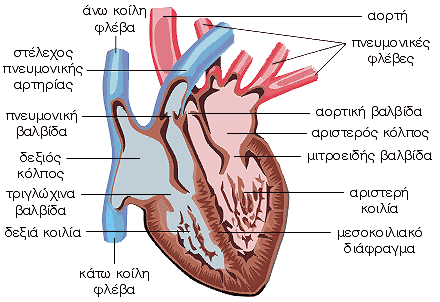
\includegraphics[width=0.8\textwidth]{misc/heart-anatomy.png}
    \caption{Εσωτερική όψη καρδιάς}
    \label{fig:2.1}
\end{figure}
\noindent Η καρδιά συντονίζεται από εσωτερικούς φυσικούς βηματοδότες, οι οποίοι είναι ο \emph{φλεβόκομβος}, που βρίσκεται στο τοίχωμα του δεξιού κόλπου και ο \emph{κολποκοιλιακός κόμβος} που βρίσκεται στο σημείο επαφής του μεσοκολπικού με το μεσοκοιλιακό διάφραγμα.
\\[0.5 \baselineskip]
Η καρδιά, επιπλέον, διαθέτει 4 \emph{βαλβίδες} που χρησιμεύουν στο να επιτρέπουν την δίοδο του αίματος προς μία μόνο κατεύθυνση και να εμποδίζουν την παλινδρόμηση του κατά τη διάρκεια της καρδιακής συστολής. Οι βαλβίδες αποτελούνται από μικρά αλλά ισχυρά μέρη, τις γλωχίνες, και είναι υπεύθυνες για υποχρεωτική κυκλοφορία του αίματος προς μία μοναδική κατεύθυνση.
\\
Αυτές οι βαλβίδες είναι:
\begin{itemize}
    \item η \emph{τριγλώχινη} μεταξύ δεξιού κόλπου και δεξιάς κοιλίας.
    \item η \emph{πνευμονική} μεταξύ δεξιάς κοιλίας και πνευμονικής αρτηρίας.
    \item η \emph{μιτροειδής} μεταξύ αριστερού κόλπου και αριστερής κοιλίας 
    \item η \emph{αορτική} μεταξύ αριστερής κοιλίας και αoρτής.
\end{itemize}
όπως φαίνονται στο σχήμα \ref{fig:2.2}.
\\ [0.5 \baselineskip]
Το περικάρδιο εμποδίζει την σύμπτωση των βαλβίδων, καθώς αποτελεί σημείο πρόσφυσης μεταξύ του μυοκαρδίου και των γλωχίνων των βαλβίδων, ενώ ταυτόχρονα βοηθά στον διαχωρισμό της σύσπασης κόλπων και κοιλιών, δρώντας ως μονωτής του σήματος σύσπασης. 
\begin{figure}[H]
    \centering
    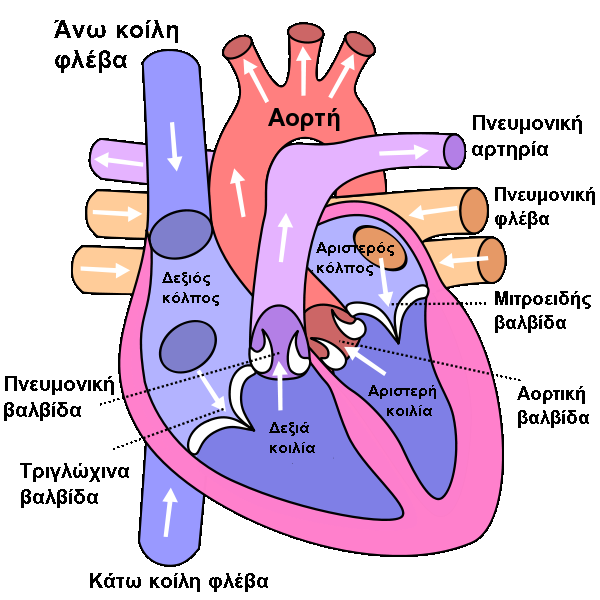
\includegraphics[width=0.7\textwidth]{misc/valves_of_heart.png}
    \caption{Κύρια μέρη της καρδιάς}
    \label{fig:2.2}
\end{figure}
\noindent Τέλος, για την αιμάτωση της, η καρδιά έχει δύο αγγεία, την αριστερή και την δεξιά \emph{στεφανιαία αρτηρία} που βρίσκονται στο αρχικό μέρος της αορτής. Ο βασικός τους ρόλος είναι να παρέχουν οξυγόνο και γενικότερα θρεπτικές ουσίες στα κύτταρα του μυοκάρδιου.
\section{Ηλεκτρική Φυσιολογία Καρδιάς}
\justifying
Ο καρδιακός μυς αποτελείται από κύτταρα που ονομάζονται \emph{καρδιακές μυϊκές ίνες}. Οι μεμβράνες των γειτονικών κυττάρων συνδέονται μεταξύ τους σε σειρά αλλά και πλάγια, δημιουργώντας ένα ενιαίο μόρφωμα. επιτρέποντας έτσι την ελεύθερη διάχυση των ιόντων. Έτσι, ο ερεθισμός και μίας μόνο μυοκαρδιακής ίνας οδηγεί σε εξάπλωση του δυναμικού δράσης σε ολόκληρη την μυϊκή μάζα.
\\[0.5 \baselineskip]
Όπως όλα τα κύτταρα του σώματος, έτσι και τα καρδιακά κύτταρα, έχουν ένα ηλεκτρικό δυναμικό στην κυτταρική τους μεμβράνη. Τόσο στον εξωκυττάριο όσο και στον ενδοκυττάριο χώρο υπάρχουν αρνητικά και θετικά φορτία (ιόντα) ίσα μεταξύ τους. Όμως, μέσα από την κυτταρική μεμβράνη υπάρχει περίσσεια αρνητικά φορτισμένων ιόντων, ενώ έξω από αυτή συγκεντρώνονται σε ίση ποσότητα θετικά φορτισμένα ιόντα. Το αποτέλεσμα είναι η \emph{πόλωση}, δηλαδή η διαφορά δυναμικού μεταξύ του εσωτερικού και του εξωτερικού της κυτταρικής μεμβράνης. Το δυναμικό αυτό ονομάζεται \emph{δυναμικό ηρεμίας} και έχει τιμή ίση με \en -90 mV.\gr
\\[2 \baselineskip]
Επιπλέον, τα καρδιακά κύτταρα είναι ικανά να μεταβάλλουν το δυναμικό της κυτταρικής τους μεμβράνης, έτσι ώστε να αναπτύξουν ένα ηλεκτρικό δυναμικό που διαδίδεται κατά μήκος της μυϊκής ίνας όταν διεγείρεται επαρκώς. Το δυναμικό αυτό είναι γνωστό ως \emph{δυναμικό δράσης}.
\\[0.5 \baselineskip]
Η καρδιά περιλαμβάνει δύο δυναμικά δράσης, ένα στο κολπικό μυοκάρδιο και ένα στο κοιλιακό μυοκάρδιο. Στο κοιλιακό μυοκάρδιο, το δυναμικό παράγεται από τα ρεύματα εκπόλωσης των γειτονικών κυττάρων και υπολογίζεται στα 105 \en mV, \gr αυξάνοντας το δυναμικό από τα -90 \en mV \gr στα περίπου 20 \en mV. \gr Μετά από το αρχικό έπαρμα, η μεμβράνη μένει σε κατάσταση εκπόλωσης για 0.15 δευτερόλεπτα στο κολπικό μυοκάρδιο έως και 0.3 δευτερόλεπτα στο κοιλιακό μυοκάρδιο, εμφανίζοντας ένα χαρακτηριστικό \en "plateau", \gr στο τέλος του οποίου ακολουθεί απότομη επαναπόλωση.
\\[0.5 \baselineskip]
Σε φυσιολογικές συνθήκες, η μυϊκή ίνα βρίσκεται σε κατάσταση ηρεμίας ή πόλωσης. Εάν διεγερθεί το ένα άκρο της με κάποιο ερέθισμα τότε ξεκινά αυτόματα η διαδικασία της εκπόλωσης και το ερέθισμα μεταφέρεται από το ένα άκρο της στο άλλο. Έπειτα ξεκινά απότομα το κύμα επαναπόλωσης που είναι ακριβώς αντίθετο με το κύμα εκπόλωσης.
\\[0.5 \baselineskip]
\begin{figure}[H]
    \centering
    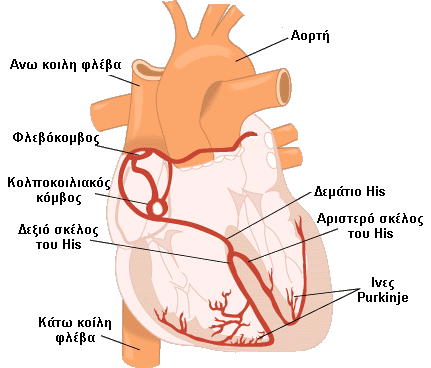
\includegraphics[width=0.7\textwidth]{misc/stimulus.png}
    \caption{Το ερεθισματαγωγό σύστημα της καρδιάς}
    \label{fig:2.3}
\end{figure}
Το ερεθισματωγό σύστημα της καρδίας (Σχήμα \ref{fig:2.3}) αποτελείται από τα εξής μέρη:
\begin{itemize}
    \item τον \emph{φλεβοκολπικό} και \emph{κολποκοιλιακό κόμβο}
    \item το κολποκοιλιακό \emph{δεμάτιο \en Hiss \gr} που χωρίζεται σε δεξί και αριστερό σκέλος
    \item τις \emph{ίνες του \en Purkinje \gr}
    \item τον \emph{φλεβόκομβο}
\end{itemize}
Ο φλεβόκομβος παράγει το πρώτο ηλεκτρικό δυναμικό, το οποίο ξεκινά αλυσιδωτή ηλεκτρική αντίδραση για την μετάδοση του ερεθίσματος σε όλο το τοίχωμα των κόλπων με αποτέλεσμα την σύσπαση τους. Η μετάδοση του ερεθίσματος στους κόλπους εξαπλώνεται σε 0.1 δευτερόλεπτα. Κατόπιν, περνά τον κολποκοιλιακό κόμβο και διαχέεται με μικρή καθυστέρηση στο δεμάτιο του \en Hiss \gr και ύστερα στις κοιλίες μέσω του δεξιού και αριστερού σκέλους του δεματίου, δημιουργώντας τους συστολή. Οι τελικές απολήξεις των στελεχών είναι οι ίνες του \en Purkinje, \gr οι οποίες προχωρούν κάθετα από το ενδοκάρδιο στο επικάρδιο.
\\[0.5 \baselineskip]
Η περίοδος από το τέλος μιας καρδιακής συστολής έως το τέλος της επόμενης ονομάζεται \emph{καρδιακός κύκλος}. Κάθε κύκλος ξεκινά με την αυτόματη παραγωγή ενός δυναμικού δράσης στον φλεβόκομβο και ολοκληρώνεται μετά το πέρας των 5 ακόλουθων φάσεων:
\begin{enumerate}
    \item την παθητική πλήρωση της καρδίας από αίμα
    \item την συστολή των κόλπων
    \item την διέγερση και ισομετρική συστολή 
    \item την εξώθηση του αίματος από την καρδιά
    \item την ισομετρική χάλαση
\end{enumerate}
\section{Ηλεκτροκαρδιογράφημα}
\justifying
Το \emph{ηλεκτροκαρδιογράφημα} ή \en \emph{ECG} \gr\cite{heart:26} είναι μία γραφική αναπαράσταση της εκπόλωσης και της επαναπόλωσης της καρδιάς, που καταγράφεται ως το δυναμικό που προκαλούν οι παραπάνω λειτουργίες και το οποίο διαδίδεται στην επιφάνεια του δέρματος.
\\[0.5 \baselineskip]
Ένα φυσιολογικό ηλεκτροκαρδιογράφημα φαίνεται στο σχήμα \ref{fig:2.4} και αποτελείτε από τα ακόλουθα διαστήματα και επάρματα:
\begin{figure}[H]
    \centering
    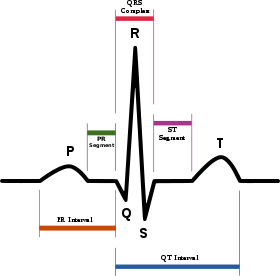
\includegraphics[width=0.7\textwidth]{misc/ECG.png}
    \caption{Χαρακτηριστικά μεγέθη ηλεκτροκαρδιογραφήματος}
    \label{fig:2.4}
\end{figure}
\begin{itemize}
    \item το \textbf{έπαρμα \en P\gr} που αντιστοιχεί στην κολπική εκπόλωση και έχει διάρκεια μικρότερη των 0.12 δευτερολέπτων. Ενίοτε εμφανίζεται θετικό ενώ άλλες φορές αρνητικό.
    \item το \textbf{διάστημα \en PR\gr} που αντιστοιχεί στο χρονικό διάστημα από την εκπόλωση των κόλπων έως την εκπόλωση των κοιλιών και για φυσιολογικά άτομα έχει διάρκεια από 0.12 έως 0.2 δευτερόλεπτα.
    \item το \textbf{σύμπλεγμα \en QRS\gr} το οποίο αντιστοιχεί στον ερεθισμό και στην εκπόλωση των κοιλιών και για φυσιολογικά άτομα έχει διάρκεια μικρότερη ή ίση των 0.10 δευτερολέπτων.
    \item το \textbf{διάστημα \en ST\gr} και το \textbf{έπαρμα \en T\gr} που αντιστοιχούν στην επαναπόλωση των κοιλιών. 
    
\end{itemize}


\gr 
\chapter{\textbf{Άνάλυση Ανεξάρτητων Συνιστωσών (\en ICA)}} \label{ch:ch3}
\gr 
\justifying
\section{Ορισμός} \label{sec:3.1}
Έστω ότι έχουμε ένα \en BSS \gr μοντέλο \en $\mathbf{X} = \mathbf{A} \mathbf{S}$ \gr όπου \en $\mathbf{X} = \begin{bmatrix}x_1 & x_2 & \ldots & x_n \end{bmatrix}^T$, $\mathbf{S} = \begin{bmatrix} s_1 & s_2 & \ldots & s_n \end{bmatrix}^T$, $\mathbf{A} \in \mathbb{R}^{n \times n}$ \gr και θέλουμε να βρούμε εκείνο τον γραμμικό συνδυασμό, \en $\mathbf{\hat{S}} = \mathbf{W} \mathbf{X}$, \gr ώστε οι παρατηρήσεις \en $\mathbf{\hat{S}}$ \gr να είναι στατιστικώς ανεξάρτητες. Αυτό είναι το πρόβλημα που επιλύει η \emph{ανάλυση ανεξαρτήτων συνιστωσών} \en (Independent Component Analysis) \cite{ica:6}, \cite{ica:7}.
\\ 
\gr Για να είμαστε σίγουροι ότι το μοντέλο \en ICA \gr μπορεί να εκτιμήσει τα σήματα πηγών κάνουμε τις ακόλουθες υποθέσεις:
\begin{itemize}
    \item Τα σήματα πηγών του πίνακα \en $\mathbf{S}$ \gr είναι \emph{στατιστικώς ανεξάρτητα}.
    \item Οι ανεξάρτητες συνιστώσες να ακολουθούν μη Γκαουσιανές κατανομές, καθώς στην περίπτωση Γκαουσιανών κατανομών οι ροπές ανώτερης τάξης είναι μηδενικές και κατά συνέπεια η εφαρμογή του αλγορίθμου \en ICA \gr είναι αδύνατη.
    \item Ο πίνακας μίξης \en $\mathbf{A}$ \gr είναι τετραγωνικός καθώς κατά την εκτίμηση του πίνακα \en $\mathbf{A}$, \gr μπορούμε να υπολογίσουμε τις ανεξάρτητες συνιστώσες από την αντιστροφή του, δηλαδή: \en
    \begin{align*}
        \mathbf{\hat{S}} = \mathbf{A}^{-1} \mathbf{X}
    \end{align*}
\end{itemize}
\gr Επίσης, για να μειώσουμε την πολυπλοκότητα του \en ICA, \gr θα κάνουμε κάποιες επιπλέον υποθέσεις:
\begin{itemize}
    \item Οι πηγές να έχουν μηδενικό μέσο όρο. Σε περίπτωση που είναι διάφορος του μηδενός, αφαιρούμε το μέσο όρο από τις παρατηρούμενες μεταβλητές \en $\mathbf{X}$ \gr καθώς και οι ανεξάρτητες συνιστώσες \en $\mathbf{\hat{S}}$ \gr θα έχουν και αυτές μηδενική μέση τιμή.
    \item Οι πηγές να έχουν πίνακα συσχέτισης ίσο με τον μοναδιαίο καθώς περιορίζει την εύρεση του πίνακα μίξης σε εύρεση ορθογώνιου πίνακα. Αν δεν είναι μοναδιαίος, μπορούμε να κάνουμε λεύκανση δεδομένων. 
\end{itemize}
Από τις πολλές μεθόδους που αναφέρονται στο \cite{ica:6}, θα ασχοληθούμε με τον αλγόριθμο \en FastICA \gr που έχει ως κριτήριο την μεγιστοποίηση της μη-γκαουσιανότητας, και συγκεκριμένα με την χρήση της αρνητικής εντροπίας.
% ta meionekthmata sto pararthma 
\section{Βοηθητικές Έννοιες} \label{sec:3.2}
\subsection{Μη Γκαουσιανότητα} \label{sec:3.2.1}
Για να αποφανθούμε για την μη γκαουσιανότητα, θα πρέπει να παραθέσουμε το ακόλουθο θεώρημα \cite{cltheorem:8}.
\begin{theorem} \label{th:3.1} [Κεντρικό Οριακό Θεώρημα]
Έστω η ακολουθία \en n \gr ανεξάρτητων τυχαίων μεταβλητών \en $X_1, X_2, \ldots, X_n$ που ακολουθούν την ίδια κατανομή, με μέση τιμή \en $E\{X_i\} = \mu$ \gr και διασπορά \en $ Var\{X_i\} = \sigma ^2 < \infty, \quad i = 1,2,\ldots,n$. \gr Τότε, καθώς το \en $n \rightarrow \infty $, η τυχαία μεταβλητή \en
\begin{align*}
    Z = \frac{1}{\sqrt{n \sigma^2}} \sum\limits_{i=1}^{n} \left ( X_i - \mu \right )
\end{align*}
\gr θα ακολουθεί ασυμπτωτικά την τυπική κανονική κατανομή $\mathcal{N}(0,1)$.
\end{theorem} 
Με άλλα λόγια, το άθροισμα δύο ανεξάρτητων τυχαίων μεταβλητών έχει συνήθως κατανομή πιο κοντά στην κανονική από οποιαδήποτε κατανομή των δύο αρχικών τυχαίων μεταβλητών.
\\ [0.5\baselineskip]
Ας υποθέσουμε τώρα ότι το διάνυσμα \en $x = \mathbf{A} s$ \gr είναι ένας συνδυασμός ανεξάρτητων συνιστωσών και για λόγους ευκολίας, υποθέτουμε ότι οι ανεξάρτητες συνιστώσες έχουν πανομοιότυπες κατανομές. Για να υπολογίσουμε μια από τις ανεξάρτητες συνιστώσες, θεωρούμε 
\begin{align*}
    y = w^T x = q^T s, \quad q = \mathbf{A}^T w
\end{align*}
έναν γραμμικό συνδυασμό των \en $x_i$ \gr με \en $w$ \gr το διάνυσμα που πρέπει να προσδιορίσουμε.
\\
Αν το \en $w$ \gr ήταν μια γραμμή του πίνακα \en $\mathbf{A}^{-1}$, \gr τότε ο γραμμικός συνδυασμός \en $y$ \gr θα ήταν ίσος με μια ανεξάρτητη συνιστώσα. Στην πράξη όμως, επειδή δεν γνωρίζουμε τον πίνακα \en $\mathbf{A}$, \gr μπορούμε να βρούμε μια εκτίμηση αυτού.
\\[0.5 \baselineskip]
Σύμφωνα με την σχέση \en $y = q^T s$, \gr  το \en $y$ \gr αποτελεί γραμμικό συνδυασμό των \en $s_i$, \gr με βάρη που δίνονται από τα \en $q_i$. \gr Σύμφωνα λοιπόν με το Κεντρικό Οριακό Θεώρημα, αφού το άθροισμα δύο ανεξάρτητων τυχαίων μεταβλητών είναι περισσότερο γκαουσιανό από τις αρχικές τυχαίες μεταβλητές, το \en $q^T s$ \gr θα είναι περισσότερο γκαουσιανό από οποιοδήποτε \en $s_i$ \gr και λιγότερο γκαουσιανό όταν στην πραγματικότητα γίνεται ίσο με ένα από τα \en $s_i$. \gr Σε αυτή την περίπτωση, μόνο ένα από τα \en $q_i$ \gr είναι μη μηδενικό.
\\[0.5 \baselineskip]
Επομένως, μπορούμε να θεωρήσουμε το \en $w$ \gr ως το διάνυσμα που μεγιστοποιεί την μη-γκαουσιανότητα του \en $w^T x$. \gr Ένα τέτοιο διάνυσμα θα ανταποκρινόταν αναγκαστικά σε ένα διάνυσμα \en $ q = \mathbf{A}^T w $ \gr το οποίο θα έχει μόνο μια μη μηδενική συνιστώσα. Αυτό σημαίνει ότι το \en $w^T x = q^T s$ \gr αποτελεί μια ανεξάρτητη συνιστώσα.
\subsection{Αρνητική Εντροπία} \label{sec:3.2.2}
Ένα μέτρο της μη προσαρμογής μιας κατανομής σε γκαουσιανή δίνεται από την αρνητική εντροπία (\en Negentropy). \gr Η αρνητική εντροπία βασίζεται στην ποσότητα της εντροπίας που προέρχεται από την θεωρία πληροφοριών \cite{entropy:9}.
\begin{definition} \label{def:3.1}
Η \emph{εντροπία} \en $\mathbf{H}$ \gr μίας τυχαίας διακριτής μεταβλητής \en $\mathbf{X}$ \gr ορίζεται ως : 
\begin{align*}
    \mathbf{H}(X) = -\sum\limits_{x \in X} p(x) \log p(x)
\end{align*}
\gr όπου τα \en $x$ \gr αποτελούν πιθανές τιμές της \en $X$. 
\end{definition}
\begin{definition} \label{def:3.2}
Η \emph{διαφορική εντροπία} \en $\mathbf{H}$ \gr μίας τυχαίας μεταβλητής \en $X$ \gr με συνάρτηση πυκνότητας πιθανότητας \en $f(x)$ \gr είναι:
\begin{align*}
    \mathbf{H}(X) = - \int f(x) \log f(x) dx
\end{align*}
\end{definition}
\gr Η εντροπία μιας τυχαίας μεταβλητής είναι συνυφασμένη με την πληροφορία που δίνει μια παρατήρηση μιας μεταβλητής. Όσο πιο απρόβλεπτη είναι μια μεταβλητή, τόσο μεγαλύτερη είναι η εντροπία της.
\\ [0.5 \baselineskip]
Ένα θεμελιώδες συμπέρασμα στην θεωρία πληροφορίας είναι ότι μια γκαουσιανή τυχαία μεταβλητή έχει την μεγαλύτερη εντροπία ανάμεσα σε όλες τις τυχαίες μεταβλητές που έχουν την ίδια διασπορά. Αυτό σημαίνει ότι η εντροπία μπορεί να χρησιμοποιηθεί ως μέτρο της μη γκαουσιανότητας. Στην πραγματικότητα, αυτό δείχνει ότι η γκαουσιανή κατανομή είναι πιο 'τυχαία' ή λιγότερο δομημένη από τις υπόλοιπες τυχαίες μεταβλητές.
\\ [0.5 \baselineskip]
Για να αποκτήσουμε ένα μέτρο της μη γκαουσιανότητας που να είναι ίσο με το μηδέν για γκαουσιανή τυχαία μεταβλητή και πάντα μη αρνητικό, με βάση την διαφορική εντροπία, ορίζουμε την \emph{αρνητική εντροπία}
\begin{definition} \label{def:3.3}
Η \emph{αρνητική εντροπία} \en $\mathbf{J}$ \gr ορίζεται ως: \en
\begin{align*}
    \mathbf{J}(X) = \mathbf{H}(X_{gauss}) - \mathbf{H}(X)
\end{align*}
\gr όπου \en $X_{gauss}$ \gr είναι μια γκαουσιανή τυχαία μεταβλητή με διασπορά ίση με την μεταβλητή \en $X$.
\end{definition}
\gr Με βάση τον Ορισμό \ref{def:3.3}, η αρνητική εντροπία είναι μηδενική όταν η τυχαία μεταβλητή \en $X$ \gr είναι γκαουσιανή και θετική στις υπόλοιπες περιπτώσεις. Επιπλέον, η αρνητική εντροπία παραμένει αμετάβλητη σε γραμμικούς αντιστρέψιμους μετασχηματισμούς, όπως ο \en PCA \gr και ο μετασχηματισμός λεύκανσης. Τέλος, το πλεονέκτημα της χρήσης της αρνητικής εντροπίας ως κριτήριο της μη γκαουσιανότητας είναι ότι η αρνητική εντροπία είναι καλά τεκμηριωμένη από την στατιστική θεωρία καθώς όσον αφορά τις στατιστικές ιδιότητες, αποτελεί τον βέλτιστο εκτιμητή της μη προσαρμογής σε γκαουσιανή.
\newpage
\noindent Το μειονέκτημα όσον αφορά την αρνητική εντροπία μιας τυχαίας μεταβλητής είναι ότι για τον ακριβή υπολογισμό της χρειάζεται την εκτίμηση της συνάρτησης πυκνότητας πιθανότητας της. Για την αποφυγή της παραπάνω διαδικασίας χρησιμοποιείται η ακόλουθη προσέγγιση \cite{ica:6}: \en
\begin{align} \label{eq:3.2.1}
    \mathbf{J}(X) \approx \left [ E\{ G(X)\} - E\{G(V)\} \right ]^2
\end{align}
\gr όπου \en $V$ \gr είναι μια γκαουσιανή τυχαία μεταβλητή με μηδενική μέση τιμή και μοναδιαία διασπορά και \en $G(.)$ \gr μια μη τετραγωνική συνάρτηση. Επίσης, υποθέτουμε ότι η τυχαία μεταβλητή \en $X$ \gr έχει και αυτή μηδενική μέση τιμή και μοναδιαία διασπορά και επιπλέον η κατανομή της \en $X$ \gr  πρέπει να είναι συμμετρική.
\\ [0.5 \baselineskip]
Το μόνο ζήτημα που προκύπτει με την \eqref{eq:3.2.1} είναι ότι με την κατάλληλη επιλογή της συνάρτησης \en $G$ \gr προκύπτουν καλύτερες προσεγγίσεις της \en $J$. \gr Συγκεκριμένα επιλέγονται συναρτήσεις οι οποίες δεν μεταβάλλονται πολύ γρήγορα, όπως: \en
\begin{subequations}
\begin{align}
&G(x) = \frac{1}{a} \log (\cosh (ax)) \quad 1 \leq a \leq 2 \label{eq:3.2.2a} \\
&G(x) = - \exp (- \frac{x^2}{2}) \label{eq:3.2.2b} \\
&G(x) = \frac{1}{4} x^4 \label{eq:3.2.2c}
\end{align}
\end{subequations} \gr
\section{Αλγόριθμος \en FastICA} \label{sec:3.3}
\gr Ο αλγόριθμος \en FastICA \gr \cite{ica:10} αποτελεί έναν \en fixed-point \gr αλγόριθμο, ο οποίος βρίσκει μια διεύθυνση, με άλλα λόγια ένα διάνυσμα \en $w$, \gr έτσι ώστε η προβολή του \en $w^T x$ \gr να μεγιστοποιεί την μη γκαουσιανότητα.
\\ [0.5 \baselineskip]
Με τον όρο \en fixed-point, \gr ένας αλγόριθμος υλοποιεί ένα μεγάλο μέρος των υπολογισμών σε ένα μόνο βήμα του. Αυτό έχει σαν αποτέλεσμα ότι τέτοιοι αλγόριθμοι, όπως και ο \en FastICA, \gr μπορούν να υλοποιηθούν παράλληλα, είναι υπολογιστικά απλοί και χρησιμοποιούν λίγη μνήμη.
\\ [0.5 \baselineskip]
Η μη γκαουσιανότητα μετριέται μέσω της προσέγγισης της αρνητικής εντροπίας \eqref{eq:3.2.1}. Επιπλέον, υπάρχει ο περιορισμός ότι η διασπορά του \en $w^T x$ \gr πρέπει να είναι μοναδιαία. Για λευκά δεδομένα, αυτό ισοδυναμεί με τον περιορισμό ότι το μέτρο του διανύσματος \en $w$ \gr να είναι ίσο με την μονάδα.
\\ [0.5 \baselineskip]
Ο υπολογισμός μιας ανεξάρτητης συνιστώσας μέσω του αλγορίθμου \en FastICA \gr είναι ο ακόλουθος, με την απόδειξη του να αναφέρετε στο \cite{ica:10}:
\begin{enumerate}
    \item Επιλογή ενός τυχαίου διανύσματος \en $w$ με μοναδιαίο μέτρο.
    \item Θέτουμε \en $ w \leftarrow E\left\{ x g(w^T x) \right\} - E\left\{ g^{'}(w^T x)  \right\} w$\gr
    \item Κανονικοποιούμε \en $w \leftarrow \frac{w}{\parallel w \parallel }$  \gr 
    \item Αν ο αλγόριθμος δεν συγκλίνει, τότε επιστρέφουμε στο βήμα 2.
\end{enumerate}
Οι συναρτήσεις \en $g$ \gr και \en $g^{'}$ \gr αποτελούν την πρώτη και την δεύτερη παράγωγο αντίστοιχα των συναρτήσεων \en $G$ \gr που ορίσαμε στις σχέσεις \en \eqref{eq:3.2.2a} - \eqref{eq:3.2.2c} \gr, δηλαδή: \en
\begin{subequations}
\begin{align}
    &g_{1}(x) = \tanh (ax), \quad g_{1}^{'}(x) = a \left[ 1-\tanh^{2}(x) \right] \quad 1 \leq a \leq 2 \label{eq:3.3.1a} \\
    &g_{2}(x) = x \exp ( -\frac{x^2}{2}), \quad g_{2}^{'} = \left( 1-x^2 \right) \exp ( -\frac{x^2}{2})  \label{eq:3.3.1b} \\
    &g_{3}(x) = x^3, \quad g_{3}^{'} = 3x^2 \label{eq:3.3.1c}
\end{align}
\end{subequations}
\gr Η σύγκλιση, σε αυτήν την περίπτωση, σημαίνει ότι οι παλιές και νέες τιμές του \en $w$ \gr δείχνουν προς την ίδια κατεύθυνση, δηλαδή το εσωτερικό τους γινόμενο είναι περίπου ίσο με την μονάδα. Αξίζει να σημειωθεί ότι δεν είναι ανάγκη το διάνυσμα \en $w$ \gr να συγκλίνει σε ένα μόνο σημείο, αφού το \en $w$ \gr και το \en $-w$ \gr έχουν την ίδια διεύθυνση.
\\ [0.5 \baselineskip]
Η παραπάνω διαδικασία δεν αποτελεί μια αξιόπιστη μέθοδο ως προς την εύρεση ανεξάρτητων συνιστωσών καθώς χρησιμοποιούμε πάρα πολλές αρχικές συνθήκες για κάθε μια συνιστώσα και υπάρχει περίπτωση δύο διαφορετικά διανύσματα να συγκλίνουν στο ίδιο μέγιστο. 
\\ [0.5 \baselineskip]
Κάνοντας ένα μετασχηματισμό λεύκανσης στα δεδομένα, παρατηρούμε ότι τα διανύσματα \en $w_i$ \gr είναι μεταξύ τους ορθογώνια. Με άλλα λόγια, η ανεξαρτησία των συνιστωσών προϋποθέτει ότι τα δεδομένα μας είναι ασυσχέτιστα που μεταφράζεται σε ορθογωνιότητα, κάνοντας \en data whitening. \gr Άρα, για να υπολογίσουμε κάποιες ανεξάρτητες συνιστώσες, πρέπει να τρέξουμε τον αλγόριθμο \en FastICA \gr αρκετές φορές και σε κάθε επανάληψη να κάνουμε τα διανύσματα \en $w_i$ \gr ορθογώνια μεταξύ τους. 
\\ [0.5 \baselineskip]
Με τις παρακάτω μεθόδους, επιτυγχάνετε η αποσυσχέτιση των ανεξαρτήτων συνιστωσών:
\begin{itemize}
    \item \textbf{\en Deflation \gr μέθοδος}
    \\ 
    Η μέθοδος αυτή βασίζεται στη ορθοκανονικοποίηση \en Gram-Schmidt \cite{gram-smidt:11} \gr που σημαίνει ότι υπολογίζουμε τις ανεξάρτητες συνιστώσες μία προς μία. Όταν έχουμε υπολογίσει \en $p$ \gr ανεξάρτητες συνιστώσες ή \en $p$ \gr διανύσματα \en $w_1, w_2, \ldots, w_p$, \gr εφαρμόζουμε τον αλγόριθμο \en FastICA \gr για τον υπολογισμό του \en $w_{p+1}$ \gr και μετά από κάθε επανάληψη, αφαιρούμε από το \en $w_{p+1}$ \gr τις προβολές των προηγούμενων \en $p$ \gr διανυσμάτων \en $ \left ( w_{p+1}^T w_{j} \right ) w_{j} , j = 1, 2, \ldots, p$ \gr και το κανονικοποιούμε. Δηλαδή: \en
    \begin{align} \label{eq:3.3.2}
        w_{p+1} \leftarrow w_{p+1} - \sum\limits_{j=1}^{p} \left( w_{p+1}^T w_j  \right)w_j
    \end{align}
    \gr και \en
    \begin{align} \label{eq:3.3.3}
        w_{p+1} \leftarrow \frac{w_{p+1}} { \parallel w_{p+1} \parallel }
    \end{align}
    \gr
    \newpage
    \item \textbf{Συμμετρική προσέγγιση}
    \\
    Τα διανύσματα \en $w_i$ \gr υπολογίζονται παράλληλα, σε αντίθεση με την προηγούμενη μέθοδο, κάνοντας παράλληλη εύρεση ανεξαρτήτων συνιστωσών. Η ορθογωνοποίηση του πίνακα των διανυσμάτων \en $\mathbf{W} = \begin{bmatrix}
    w_1 & w_2 & \ldots & w_n \end{bmatrix}^T$ \gr γίνεται με τον υπολογισμό της τετραγωνικής ρίζας πινάκων: \en
    \begin{align} \label{3.3.4}
        \mathbf{W} \leftarrow \left ( \mathbf{W} \mathbf{W}^T  \right ) ^{-\frac{1}{2}} \mathbf{W}
    \end{align}
    \gr όπου ο πίνακας \en $ \left ( \mathbf{W} \mathbf{W}^T  \right )^{-\frac{1}{2}} $ \gr λαμβάνεται, σύμφωνα με το Θεώρημα \ref{th:1.4}, ως \en $\mathbf{V} \mathbf{D}^{-\frac{1}{2}} \mathbf{V}^T$, \gr με \en $\mathbf{D}$ \gr τον διαγώνιο πίνακα των ιδιοτιμών και \en $\mathbf{V}$ τον πίνακα των ιδιοδιανυσμάτων.
    \\ 
    Μια πιο απλή εναλλακτική μέθοδος είναι επίσης η εξής διαδικασία:
    \begin{enumerate}
        \item Θέτουμε \en $\mathbf{W} \leftarrow \frac{\mathbf{W}}{\parallel \mathbf{W} \parallel}$  \gr
        \item Θέτουμε \en $\mathbf{W} \leftarrow \frac{3}{2} \mathbf{W} - \frac{1}{2} \mathbf{W} \mathbf{W}^T  \mathbf{W}$ \gr 
        \item Εάν ο πίνακας \en $\mathbf{W} \mathbf{W}^T $ \gr δεν είναι κοντά στον μοναδιαίο, τότε επιστροφή στο βήμα 2.
    \end{enumerate}
\end{itemize}
\section{Μεθοδολογία} \label{sec:3.4}
\justifying
Σε αυτήν την εργασία, θα υλοποιήσουμε τον αλγόριθμο \en FastICA \gr και με τις δύο προσεγγίσεις που αναφέραμε στο Κεφάλαιο
\ref{sec:3.3}. 
\\
Για την \en Deflation \gr προσέγγιση, ο αλγόριθμος που θα υλοποιήσουμε είναι ο εξής:
\begin{enumerate}
    \item Αφαιρούμε τον μέσο όρο από τα δεδομένα μας: \en $x \leftarrow x - m_x $ \gr
    \item Κάνουμε λεύκανση στα δεδομένα: \en $z = \left ( \mathbf{D}^{- \frac{1}{2}} \mathbf{V}^T \right)x $ \gr 
    \item Επιλέγουμε \en $m$ \gr ανεξάρτητες συνιστώσες για να εκτιμήσουμε.
    \item Θέτουμε τον μετρητή \en $p \leftarrow 1$ \gr
    \item Επιλέγουμε τυχαία ένα αρχικό διάνυσμα \en $w_p$ \gr με μοναδιαίο μέτρο.
    \item Θέτουμε \en $w_p \leftarrow E \left \{ z g( w_p^T z) \right \} - E \left \{ g^{'}(w_p^T z) \right \}w_p $, \gr όπου οι συναρτήσεις \en $g, g^{'} $ \gr ορίζονται από τις σχέσεις \en \eqref{eq:3.3.1a} - \eqref{eq:3.3.1c} \gr.
    \item Κάνουμε την παρακάτω ορθογωνοποίηση: \en
    \begin{align*}
        w_p \leftarrow w_p - \sum\limits_{j=1}^{p-1} \left (
        w_p^T w_j\right ) w_j
    \end{align*} \gr
    \item Κανονικοποιούμε \en $w_p \leftarrow \frac{w_p}{\parallel w_p \parallel} $ \gr
    \item Εάν το διάνυσμα \en $w_p$ \gr δεν έχει συγκλίνει, επιστρέφουμε στο βήμα 6.
    \item Αυξάνουμε το μετρητή \en $p \leftarrow p+1 $. \gr  
    Εάν \en $p \leq m$ , \gr επιστρέφουμε στο βήμα 5. 
\end{enumerate} \leavevmode
ενώ για στην Συμμετρική προσέγγιση:
\begin{enumerate}
    \item Αφαιρούμε τον μέσο όρο από τα δεδομένα μας: \en $x \leftarrow x - m_x $ \gr
    \item Κάνουμε λεύκανση στα δεδομένα: \en $z = \left ( \mathbf{D}^{- \frac{1}{2}} \mathbf{V}^T \right)x $ \gr 
    \item Επιλέγουμε \en $m$ \gr ανεξάρτητες συνιστώσες για να εκτιμήσουμε.
    \item Επιλέγουμε αρχικές συνθήκες για τα διανύσματα \en $w_i \gr , i = 1, 2, \ldots, m$ \gr με μόνη συνθήκη να έχουν όλα μοναδιαίο μέτρο.
    \item Κάνουμε συμμετρική ορθογωνοποίηση του πίνακα \en $\mathbf{W} = \begin{bmatrix} w_1 & \ldots & w_m \end{bmatrix}^T$ :
    \begin{align*}
        \mathbf{W} \leftarrow \left ( \mathbf{W} \mathbf{W}^T \right)^{-\frac{1}{2}} \mathbf{W}    
    \end{align*} \gr
    \item Για κάθε \en $i = 1, \ldots, m$, \gr 
    θέτουμε \en $w_i \leftarrow E \left \{ z g( w_i^T z) \right \} - E \left \{ g^{'}(w_i^T z) \right \}w_i $, \gr όπου οι συναρτήσεις \en $g, g^{'} $ \gr ορίζονται από τις σχέσεις \en \eqref{eq:3.3.1a} - \eqref{eq:3.3.1c} \gr.
    \item Κάνουμε ορθογωνοποίηση όπως το βήμα 4.
    \item Εάν ο πίνακας δεν συγκλίνει, επιστρέφουμε στο βήμα 6.
\end{enumerate}
Οι παραπάνω διαδικασίες υλοποιήθηκαν στους κώδικες \en fastica.py, deflational\_method.py \gr  και \en symmetric\_mehod.py \gr που βρίσκονται στο παράρτημα.


\chapter{\textbf{Ανάλυση Περιοδικών Συνιστωσών(π\en{CA})}} \label{ch:ch4}
\section{Ορισμός}
\justifying
Υποθέτουμε ένα \en{BSS} (\en{Blind Source Separation}) σύστημα το οποίο περιέχει σήματα από \en n \gr διαφορετικούς αισθητήρες με \en m δείγματα από τον κάθε αισθητήρα. Επίσης, υποθέτουμε ότι ο αριθμός των δειγμάτων \en{m} είναι πολύ μεγαλύτερος από τον αριθμό των αισθητήρων \en{n}, δηλαδή ότι \en{m} $\gg$ \en{n}.
\\ \\
Συμβολίζουμε με $x(t) = {\begin{bmatrix} 
    x_1(t) & x_2(t) & \ldots &  x_n(t)
    \end{bmatrix}}^T \in \mathbb{R}^{n\times1} $
το διάνυσμα των σημάτων που λαμβάνουμε από τους αισθητήρες την χρονική στιγμή t, τα οποία και δειγματοληπτούμε με περίοδο δειγματοληψίας $T_s$. Ο πίνακας των σημάτων θα είναι ο $\textbf{X}\in \mathbb{R}^{m\times n}$, με στήλες που αντιστοιχούν στα σήματα του κάθε αισθητήρα και γραμμές που αντιστοιχούν στα δείγματα. Παραδείγματος χάρη, το στοιχείο $x_{ij}$ περιέχει την μέτρηση του i δείγματος για το σήμα που λαμβάνουμε από τον j αισθητήρα. Επίσης, συμβολίζουμε με $\textbf{X}_{k} \in \mathbb{R}^{m\times1}$ το διάνυσμα με όλα τα δείγματα που αντιστοιχούν στον k αισθητήρα και με $x_k \in \mathbb{R}^{n\times1}$ το διάνυσμα που περιέχει τα δείγματα από όλους τους αισθητήρες την $kT_s$ χρονική στιγμή.
\\
Άρα ο πίνακας $\textbf{X}$ μπορεί να γραφεί ως εξής:
\begin{align}\label{eq:4.1.1}
 \textbf{X} = \begin{bmatrix} 
                    \mathbf{X}_1 && \mathbf{X}_2 && \ldots && \mathbf{X}_n
                \end{bmatrix} = \begin{bmatrix} 
    x_1 && x_2 && \ldots && x_m
 \end{bmatrix}^T  
\end{align}
\\
Βάσει του μοντέλου \en{BSS}, τα σήματα $x(t)$ αποτελούν γραμμικούς συνδυασμούς κάποιων πηγαίων σημάτων $s(t) = {\begin{bmatrix} 
    s_1(t) & s_2(t) & \ldots &  s_n(t)
    \end{bmatrix}}^T \in \mathbb{R}^{n\times1} $ 
που αντιστοιχούν σε πίνακα δεδομένων $\textbf{S} \in \mathbb{R}^{m\times n}$. Με άλλα λόγια:
\begin{align}\label{eq:4.1.2}
 \mathbf{X} = \mathbf{S}\mathbf{B} 
\end{align}
 όπου $\mathbf{B} \in \mathbb{R}^{n\times n}$ ένας αντιστρέψιμος πίνακας που ονομάζεται πίνακας μίξης.
\newpage
\noindent Βασική υπόθεση για την ανάλυση περιοδικών συνιστωσών είναι πως τα πηγαία σήματα $s(t)$ έχουν κάποια περιοδική δομή. Ο σκοπός μας, μέσω της παραπάνω μεθόδου, είναι η εύρεση ενός διανύσματος συντελεστών βαρύτητας
$\mathbf{w} = \begin{bmatrix} w_1 && w_2 && \ldots && w_n \end{bmatrix}^T$ που θα δίνει μια προσέγγιση των πηγαίων σημάτων ως γραμμικό συνδυασμό των σημάτων $x(t)$
$$
\hat{s}(t) = \mathbf{w}^T x(t)
$$
\\ 
 που στην περίπτωση που έχουμε διακριτά σήματα γράφεται ως:
 \begin{align}\label{eq:4.1.3}
     \hat{s} = \begin{bmatrix} \hat{s}_1 \\ \hat{s}_2 \\
     \vdots \\ \hat{s}_n
     \end{bmatrix} = \mathbf{X}\mathbf{w} ,
     \hat{s} \in \mathbb{R}^{m\times 1} \space , \mathbf{w} \in 
     \mathbb{R}^{n\times 1}
 \end{align}
 $$ \\ \hat{s}_i \in \mathbb{R} , i = 1 , 2 , \ldots , n $$
 τέτοιον ώστε να ελαχιστοποιείται η παρακάτω συνάρτηση κόστους:
 \begin{align}\label{eq:4.1.4}
     e(\tau) = \frac {E(\left | \hat{s}(t+\tau) - \hat{s}(t) \right | ^2)} {E(\left | \hat{s}(t) \right | ^2)}
 \end{align}
 δηλαδή την μέση τετραγωνική διαφορά του σήματος που θέλουμε να εξάγουμε από το μετατοπισμένο στο χρόνο κατά  $\tau$ σήμα , κανονικοποιημένο ως προς την ισχύ του. 
 \\ \\ 
 Το $e(\tau)$ ονομάζεται \textbf{σφάλμα περιοδικότητας} και εκφράζει κατά πόσο ένα σήμα είναι μη περιοδικό, ενώ η μεταβλητή $\tau$ ονομάζεται \textbf{χρονική/δειγματική καθυστέρηση} ή αλλίως \textbf{lag}.
 \\ \\
 Με βάση τα παραπάνω, παρατηρούμε ότι όσο μεγαλύτερη τιμή για την μεταβλητή $\tau$ επιλέξουμε , τόσο λιγότερα δείγματα από τα διαθέσιμα μπορούμε να χρησιμοποιήσουμε ώστε να εκτιμήσουμε την έκφραση του αριθμητή της \eqref{eq:4.1.4}. Για $\tau = kT_s$, άρα $\hat{s}_k = \hat{s}(kT_s)$ και με βάση τον ορισμό της αναμενώμενης τιμής ενός διακριτού σήματος (σχέση) % need reference
 , κατά προσέγγιση λαμβάνουμε ότι:
 $$
 Ε(\left | \hat{s}(t+\tau) - \hat{s}(t) \right |^2) = \sum_{i=1}^{m-k}
 \left | \hat{s}_{i+k} - \hat{s}_i  \right |^2
$$
$$
 E(\left | \hat{s}(t) \right |^2 ) = \sum_{i=1}^{m} \left | \hat{s}_i \right |^2
 $$
 \\
 Με βάση τα παραπάνω , ή \eqref{eq:4.1.4} γίνεται \cite{piCA:12}:
 \begin{align} \label{eq:4.1.5}
 e[k] = \frac{\sum\limits_{i=1}^{m-k}
 \left | \hat{s}_{i+k} - \hat{s}_i  \right |^2}{\sum\limits_{i=1}^{m} \left | \hat{s}_i \right |^2} \geq 0 , i = 1,2,\ldots,m-1
 \end{align}
 Όταν η παράμετρος χρονικής καθυστέρησης $k$ λαμβάνει τιμή ίση με την περίοδο του σήματος, η τιμή στον αριθμητή στην \eqref{eq:4.1.5} μηδενίζεται.Επομένως, για να μεγιστοποιήσουμε την περιοδική δομή του σήματος, πρέπει να ελαχιστοποιήσουμε το σφάλμα περιοδικότητας.
 \\
Ορίζουμε τους παρακάτω βοηθητικούς πίνακες:
$$
 \hat{s}_0[k]=\begin{bmatrix} 
                \hat{s}_1\\\hat{s}_2\\\vdots\\\hat{s}_{m-k}
                \end{bmatrix} , 
 \hat{s}_t[k] = \begin{bmatrix} 
                \hat{s}_{k+1} \\ \hat{s}_{k+2} \\ \vdots \\ \hat{s}_{m}
                \end{bmatrix}
$$
$$
 \mathbf{X}_{0}[k] = \begin{bmatrix} 
                x_{1,1}&x_{1,2}&\ldots&x_{1,n} \\
                \vdots&\vdots&\vdots&\vdots \\
                x_{m-k,1}&x_{m-k,2}&\ldots&x_{m-k,n}
                \end{bmatrix} = 
                \begin{bmatrix}
                \mathbf{X}_{01}[k] & \mathbf{X}_{02}[k] & \ldots & 
                \mathbf{X}_{0n}[k]
                \end{bmatrix} =
                \begin{bmatrix}
                x_1^T \\ x_2^T \\ \vdots \\ x_{m-k}^T
                \end{bmatrix}
$$
$$
 \mathbf{X}_{t}[k] = \begin{bmatrix} 
                x_{k+1,1} & x_{K+1,2} & \ldots & x_{K+1,n} \\
                \vdots & \vdots & \vdots & \vdots \\
                x_{m,1} & x_{m,2} & \ldots & x_{m,n}
                \end{bmatrix} = 
                \begin{bmatrix}
                \mathbf{X}_{t1}[k] & \mathbf{X}_{t2}[k] & \ldots & 
                \mathbf{X}_{tn}[k]
                \end{bmatrix} =
                \begin{bmatrix}
                x_{k+1}^T \\ x_{k+2}^T \\ \vdots \\ x_{m}^T
                \end{bmatrix}
$$
$$
\hat{s}_0[k] \in \mathbb{R}^{(m-k)\times 1} \qquad \hat{s}_t[k] \in \mathbb{R}^{(m-k)\times 1}  
$$
$$
\mathbf{X}_0[k] \in \mathbb{R}^{(m-k)\times n} \qquad \mathbf{X}_t[k] \in \mathbb{R}^{(m-k)\times n}
$$
Για τους παραπάνω πίνακες και διανύσματα, για μείωση της πολυπλοκότητας των εξισώσεων, θα παραλείπεται η μεταβλητή $k$, θεωρώντας ότι πάντοτε έχει μια συγκεκριμένη τιμή.
\\
Βάσει της \eqref{eq:4.1.2} και κάνοντας χρήση των βοηθητικών πινάκων, έχουμε:
\begin{align} \label{eq:4.1.6}
    \hat{s}_0 = \mathbf{X}_0 w \qquad \hat{s}_t = \mathbf{X}_t w
\end{align}
και, όπως γνωρίζουμε από την γραμμική άλγεβρα, για οποιοδήποτε διάνυσμα $y \in \mathbb{R}_{n\times 1}$ με στοιχεία $y_i$ ισχύει:
\begin{align} \label{eq:4.1.7}
    y^Ty = \sum_{i=1}^{n} y_i^2 = \sum_{i=1}^{n} \left | y_i \right |^2
\end{align}
Ξαναγράφουμε την \eqref{eq:4.1.5} χρησιμοποιώντας τις σχέσεις \eqref{eq:4.1.6} και \eqref{eq:4.1.7}:
\begin{equation*}
\begin{split}
e[k] &= \frac{(\hat{s}_t - \hat{s}_0)^T (\hat{s}_t - \hat{s}_0)}{\hat{s}^T \hat{s}} =
\frac{\hat{s}_t^T \hat{s}_t - \hat{s}_t^T \hat{s}_0 - \hat{s}_0^T \hat{s}_t + \hat{s}_0^T \hat{s}_0} {\hat{s}^T \hat{s}} \\
&= \frac{w^T\mathbf{X}_t^T\mathbf{X}_t w
 - w^T\mathbf{X}_t^T\mathbf{X}_0 w
 - w^T\mathbf{X}_0^T\mathbf{X}_t w
 + w^T\mathbf{X}_0^T\mathbf{X}_0 w}
 {w^T\mathbf{X}^T\mathbf{X}w} \Rightarrow \\
\end{split}
\end{equation*}
\begin{align} \label{eq:4.1.8}
    e(\mathbf{X},w,k) = \frac{w^T(\mathbf{X}_t^T\mathbf{X}_t - \mathbf{X}_t^T\mathbf{X}_0 - \mathbf{X}_0^T\mathbf{X}_t + \mathbf{X}_0^T\mathbf{X}_0)w} {w^T \mathbf{X}^T \mathbf{X} w}
\end{align}
Ορίζουμε τους παρακάτω πίνακες μαζί με τους παράγοντες κανονικοποίησης τους:
\begin{subequations}
\begin{align} 
&\mathbf{C} = \frac{1}{m} \mathbf{X}^T \mathbf{X} \quad \mathbf{C} \in \mathbb{R}^{n \times n} \\ \label{eq:4.1.9a}
&\mathbf{C}_0[k] = \frac{1}{m-k} \mathbf{X}_0^T \mathbf{X}_0 \quad \mathbf{C}_0[k] \in \mathbb{R}^{n\times n} \\ \label{eq:4.1.9b}
&\mathbf{C}_t[k] = \frac{1}{m-k} \mathbf{X}_t^T \mathbf{X}_t \quad \mathbf{C}_t[k] \in \mathbb{R}^{n\times n} \\\label{eq:4.1.9c}
&\mathbf{C}_{t0}[k] = \frac{1}{m-k} \mathbf{X}_t^T \mathbf{X}_0 \quad \mathbf{C}_{t0}[k] \in \mathbb{R}^{n\times n} \\ \label{eq:4.1.9d}
&\mathbf{A}[k] = \frac{1}{m-k}( \mathbf{X}_t^T \mathbf{X}_t - \mathbf{X}_t^T \mathbf{X}_0 - \mathbf{X}_0^T \mathbf{X}_t 
+ \mathbf{X}_0^T \mathbf{X}_0) \notag \\
& = \mathbf{C}_0[k] + \mathbf{C}_t[k] - ( \mathbf{C}_{t0}[k]+ \mathbf{C}_{t0}^T[k] ) , \quad \mathbf{A}[k] \in \mathbf{R}^{n \times n}
\end{align} \label{eq:4.1.9e} 
\end{subequations}
Βάσει των εξισώσεων \eqref{eq:4.1.9a} - \eqref{eq:4.1.9e}, η \eqref{eq:4.1.8} γίνεται:
\begin{align} \label{eq:4.1.10}
    e(\mathbf{X},w,k) = R(\mathbf{A}[k],\mathbf{C},w) = 
    \frac{w^T\mathbf{A}[k]w} {w^T \mathbf{C} w}
\end{align}
Η εξίσωση \eqref{eq:4.1.10} είναι ισοδύναμη με την εξίσωση \eqref{eq:4.1.8} και αποτελεί ένα γενικευμένο κλάσμα Rayleigh. Για σταθερό $k$, συμμετρικό πίνακα $\mathbf{A}$ και θετικά ορισμένο πίνακα $\mathbf{C}$, τότε, όπως αποδείξαμε στο Θεώρημα 1.5, η ελαχιστοποίηση του είναι ισοδύναμη με την εύρεση της μικρότερης γενικευμένης ιδιοτιμής του ζεύγους ($\mathbf{A}[k]$,$\mathbf{C}$), που υπολογίζεται από την σχέση:
\begin{align} \label{eq:4.1.11}
    \mathbf{A}[k]w = \lambda \mathbf{C} w
\end{align}
\newpage 
\noindent Η σχέση \eqref{eq:4.1.11} αποκτά την ελάχιστη τιμή της όταν το $w$ είναι το αντίστοιχο γενικευμένο ιδιοδιάνυσμα. Αν $\lambda _1 < \lambda _2 < \ldots < \lambda_n$ είναι οι γενικευμένες ιδιοτιμές, τότε η συνιστώσα που αντιστοιχεί στην ιδιοτιμή $\lambda_1$ είναι αυτή για την οποία μεγιστοποιείται η περιοδική δομή, ενώ η n-οστή ιδιοτιμή θα αντιστοιχεί στην λιγότερο αμιγώς περιοδική συνιστώσα, για μια συγκεκριμένη τιμή του $k$. Οι συνιστώσες δίνονται από τον μετασχηματισμό $\mathbf{\hat{S}} = \mathbf{X}\mathbf{W} $, όπου $\mathbf{W}$ ο πίνακας με στήλες τα γενικευμένα ιδιοδιανύσματα, ταξινομημένα από αυτό που αντιστοιχεί στην μικρότερη ιδιοτιμή στα αριστερά, μέχρι αυτό που αντιστοιχεί στην μεγαλύτερη στα δεξιά.
\\ \\
Είναι δυνατόν να έχουμε σημαντικά αποτελέσματα ακόμη και για συνιστώσες πέραν αυτής που αντιστοιχεί στην ελάχιστη ιδιοτιμή, ειδικά για πραγματικά σήματα στα οποία η περιοδικότητα του σήματος δεν είναι σταθερή. Εν γένει, τα πιο ενδιαφέροντα αποτελέσματα για όλες τις συνιστώσες δίνονται εκεί που η \eqref{eq:4.1.10}, για τη μικρότερη ιδιοτιμή, έχει τοπικά ελάχιστα ως προς το k.
\section{Προτάσεις}
\justifying
Σε αυτήν την υποενότητα, ακολουθούν κάποιες προτάσεις όσον αφορά τον αλγόριθμο πCA.
\subsection*{\small{Πρόταση 4.1}}
Οι πίνακες $\mathbf{C}$, $\mathbf{C}_0[k]$, $\mathbf{C}_t[k]$ και $\mathbf{A}[k]$ είναι \emph{συμμετρικοί}.
\subsubsection*{\small{\textit{Απόδειξη}}}
Από τις σχέσεις \eqref{eq:4.1.9a} - \eqref{eq:4.1.9e}:
$$
\mathbf{C}^T = \left ( \frac{1}{m} \mathbf{X}^T \mathbf{X} \right)^T 
    = \frac{1}{m} \mathbf{X}^T \mathbf{X} = \mathbf{C}
$$
Αν αντί για $\mathbf{X}$, έχουμε αντίστοιχα $\mathbf{X}_0$, $\mathbf{X}_t$ και $\mathbf{X}_t - \mathbf{X}_0$ και αντί για $\frac{1}{m}$ έχουμε $\frac{1}{m-k}$, αποδεικνύεται με τον ίδιο τρόπο ότι οι πίνακες $\mathbf{C}_0[k]$, $\mathbf{C}_t[k]$ και $\mathbf{A}[k]$ είναι συμμετρικοί. 
\\[0.5 \baselineskip]
\textit{Παρατήρηση}: Ο πίνακας $\mathbf{C}_{t0}[k]$ δεν είναι οπωσδήποτε συμμετρικός.
\subsection*{\small{Πρόταση 4.2}}
Οι πίνακες $\mathbf{C}$, $\mathbf{C}_0[k]$, $\mathbf{C}_t[k]$ και $\mathbf{A}[k]$ είναι τουλάχιστον \emph{θετικώς ημιορισμένοι}.
\subsubsection*{\small{\textit{Απόδειξη}}}
Παρατηρούμε ότι:
$$
w^{Τ} \mathbf{C} w = w^T \left ( \frac{1}{m} \mathbf{X}^T \mathbf{X} \right ) w = \left ( \frac{1}{\sqrt{m}} \mathbf{X} w \right )^T 
\left ( \frac{1}{\sqrt{m}} \mathbf{X} w \right ) 
= \left \|  \frac{1}{\sqrt{m}} \mathbf{X} w \right \|^2 \geq 0
$$
\newpage
\noindent Αν αντί για $\mathbf{X}$, έχουμε αντίστοιχα $\mathbf{X}_0$, $\mathbf{X}_t$ και $\mathbf{X}_t - \mathbf{X}_0$ και αντί για $\frac{1}{m}$ έχουμε $\frac{1}{m-k}$, αποδεικνύεται με τον ίδιο τρόπο ότι οι πίνακες $\mathbf{C}_0[k]$, $\mathbf{C}_t[k]$ και $\mathbf{A}[k]$ είναι θετικώς ημιορισμένοι.
\\ \\
\textit{Παρατήρηση}: Θεωρώ ότι οι στήλες του $\mathbf{X}$, δηλαδή τα παρατηρούμενα σήματα, είναι γραμμικά ανεξάρτητες. Αναγκαία συνθήκη για να ισχύει αυτό είναι να έχουμε δείγματα τουλάχιστον όσα και τα σήματα, δηλαδή $m \geq n$. Επειδή έχουμε υποθέσει ότι έχουμε πολύ περισσότερα δείγματα από αριθμό καναλιών, είναι στην πράξη αδύνατον να αντιμετωπίσουμε πρόβλημα.
\\[0.5 \baselineskip]
Εφόσον είμαστε σίγουροι ότι οι στήλες του πίνακα $\mathbf{X}$ είναι γραμμικά ανεξάρτητες, τότε $\mathbf{X} w \neq 0$, $\forall w \in \mathbb{R}^{n\times 1}$, άρα:
\begin{align*}
&\mathbf{X} w \neq 0 \Leftrightarrow \frac {1}{\sqrt{m}} \mathbf{X} w \neq 0 \Leftrightarrow \left \| \frac {1}{\sqrt{m}} \mathbf{X} w \right \| ^2 \neq 0 \\
&\left ( \frac {1}{\sqrt{m}} \mathbf{X} w \right )^T \left ( \frac {1}{\sqrt{m}} \mathbf{X} w \right ) \neq 0 \Leftrightarrow \\
& w^T \left ( \frac{1}{m} \mathbf{X}^T \mathbf{X} \right ) w \neq 0
\Leftrightarrow 
w^T \mathbf{C} w \neq 0, \forall w \neq 0 \in \mathbb{R}^{n\times 1}
\end{align*}
Από την παραπάνω σχέση συμπεραίνουμε ότι ο πίνακας $\mathbf{C}$ είναι
\emph{θετικά ορισμένος}.
\subsection*{\small{Πρόταση 4.3}}
Έστω ότι πολλαπλασιάζεται ο πίνακας δειγμάτων $\mathbf{X}$ από τα δεξιά με έναν οποιονδήποτε αντιστρέψιμο πίνακα $\mathbf{Q} \in \mathbb{R}^{n\times n}$. Τότε οι περιοδικές συνιστώσες που εξάγουμε από τον $\mathbf{X}$, για συγκεκριμένο k, είναι ίσες με αυτές που εξάγουμε από τον $\mathbf{\Tilde{X}} = \mathbf{X}\mathbf{Q}$, πολλαπλασιασμένες με κάποιον διαγώνιο πίνακα μη μηδενικών διαγωνίων στοιχείων (ίδια διεύθυνση, αλλαγή σε μέτρο ή/και πρόσημο), ενώ η συνάρτηση \eqref{eq:4.1.8} παραμένει αμετάβλητη ως προς την παράμετρο $k$.
\subsubsection*{\small{\textit{Απόδειξη}}}
Έχουμε $\mathbf{\Tilde{X}} = \mathbf{X} \mathbf{Q}$. Άρα, σύμφωνα με την \eqref{eq:4.1.6} ισχύουν οι σχέσεις $\mathbf{\Tilde{X}}_0 = \mathbf{X}_0 \mathbf{Q}$ και $\mathbf{\Tilde{X}}_t = \mathbf{X}_t \mathbf{Q}$.
Οπότε, βάσει των \eqref{eq:4.1.9a} και \eqref{eq:4.1.9e}, έχουμε:
$$
\mathbf{\Tilde{C}} = \frac{1}{m} \mathbf{\Tilde{X}}^T \mathbf{\Tilde{X}}
= \frac{1}{m} \left ( \mathbf{X} \mathbf{Q}  \right )^T \left ( \mathbf{X} \mathbf{Q}  \right ) = \mathbf{Q}^T 
\left ( \frac{1}{m} \mathbf{X}^T \mathbf{X}  \right ) \mathbf{Q} = 
\mathbf{Q}^T \mathbf{C} \mathbf{Q}
$$
\begin{align*}
\mathbf{\Tilde{A}}[k] &= \frac{1}{m-k} \left ( \mathbf{\Tilde{X}}_t - \mathbf{\Tilde{X}}_0\right )^T \left ( \mathbf{\Tilde{X}}_t - \mathbf{\Tilde{X}}_0\right )  \\
& = \frac{1}{m-k} \left ( \mathbf{X}_t \mathbf{Q} - \mathbf{X}_0 \mathbf{Q}    \right )^T \left ( \mathbf{X}_t \mathbf{Q} - \mathbf{X}_0 \mathbf{Q}    \right )  \\
& = \frac{1}{m-k} \left [ \left ( \mathbf{X}_t - \mathbf{X}_0 \right ) \mathbf{Q} \right ]^T \left [ \left ( \mathbf{X}_t - \mathbf{X}_0 \right ) \mathbf{Q} \right ]  \\
& =\mathbf{Q}^T \left [ \frac{1}{m-k} \left ( \mathbf{X}_t - \mathbf{X}_0\right )^T \left ( \mathbf{X}_t - \mathbf{X}_0\right ) \right ] \mathbf{Q} \\
&= \mathbf{Q}^T \mathbf{A}[k] \mathbf{Q}
\end{align*}
Η εξίσωση για την εύρεση των γενικευμένων ιδιοτιμών του ζεύγους ($\mathbf{\Tilde{A}}[k]$,$\mathbf{\Tilde{C}}$) ώστε να ελαχιστοποιήσουμε το αντίστοιχο κλάσμα Rayleigh είναι:
$$
\mathbf{\Tilde{A}}[k] \Tilde{w} = \Tilde{\lambda} \mathbf{\Tilde{C}} \Tilde{w} \Leftrightarrow \mathbf{Q}^T \mathbf{A}[k] \mathbf{Q} \Tilde{w} = \Tilde{\lambda} \mathbf{Q}^T \mathbf{C} \mathbf{Q} \Tilde{w}
$$
Εφόσον ο πίνακας $\mathbf{Q}$ είναι αντιστρέψιμος, πολλαπλασιάζουμε από αριστερά με τον ανάστροφο πίνακα του $\mathbf{Q}^{-1}$:
\begin{align*}
&\left ( \mathbf{Q}^{-1} \right )^T \mathbf{Q}^T \mathbf{A} \mathbf{Q} \Tilde{w} = \left ( \mathbf{Q}^{-1} \right )^T \Tilde{\lambda} \mathbf{Q}^T \mathbf{C} \mathbf{Q} \Tilde{w} \Leftrightarrow \\
&\left ( \mathbf{Q}^{-1} \right )^T \mathbf{Q}^T \mathbf{A} \mathbf{Q} \Tilde{w} = \Tilde{\lambda} \left ( \mathbf{Q}^{-1} \right )^T \mathbf{Q}^T \mathbf{C} \mathbf{Q} \Tilde{w} \Leftrightarrow \\
&\mathbb{I}_n \mathbf{A} \mathbf{Q} \Tilde{w} = \Tilde{\lambda} \mathbb{I}_n \mathbf{C} \mathbf{Q} \Tilde{w} \Leftrightarrow 
\mathbf{A}\left ( \mathbf{Q} \Tilde{w} \right) = \Tilde{\lambda} \mathbf{C} \left ( \mathbf{Q} \Tilde{w} \right )
\end{align*}
Συγκρίνοντας την παραπάνω σχέση με την $\mathbf{A} w = \lambda \mathbf{C} w$, βλέπουμε πως ο μετασχηματισμός των δεδομένων μεταφράζεται σε μετασχηματισμό των γενικευμένων ιδιοδιανυσμάτων του ζεύγους ($\mathbf{A}$,$\mathbf{C}$) για μια συγκεκριμένη τιμή του $k$. Επίσης, παρατηρούμε ότι η τιμή των γενικευμένων ιδιοτιμών διατηρείται όπως και η σειρά των γενικευμένων ιδιοδιανυσμάτων, αν τα ταξινομήσουμε βάσει των ιδιοτιμών τους, όχι όμως και η τιμή τους καθώς υπάρχει κάποια απροσδιοριστία ως προς το μέτρο των ιδιοδιανυσμάτων. Τότε, ισχυεί η σχέση: 
$$
\mathbf{W} \mathbf{P} = \mathbf{Q} \mathbf{\Tilde{W}} 
$$
όπου $\mathbf{W} \in \mathbb{R}^{n \times n}$ ο πίνακας με στήλες τα γενικευμένα ιδιοδιανύσματα του ζεύγους ($\mathbf{Α}[k]$,$\mathbf{C}$),
$\mathbf{\Tilde{W}} \in \mathbf{R}^{n \times n}$ ο πίνακας με στήλες τα αντίστοιχα γενικευμένα ιδιοδιανύσματα του ζεύγους ($\mathbf{\Tilde{Α}}[k]$,$\mathbf{\Tilde{C}}$) και $\mathbf{P} \in \mathbb{R}^{n \times n}$ ένας διαγώνιος πίνακας με πραγματικά και μη μηδενικά στοιχεία στην διαγώνιο του. Επειδή ο πίνακας $\mathbf{Q}$ είναι αντιστρέψιμός, ισχύει $\mathbf{\Tilde{W}} = \mathbf{Q}^{-1} \mathbf{W} \mathbf{P}^{-1}$, οι συνιστώσες που λαμβάνουμε από τα δεδομένα $\mathbf{\Tilde{X}} = \mathbf{X} \mathbf{Q}$ θα είναι:
\begin{align*}
\mathbf{\Tilde{\hat{S}}} &= \mathbf{\Tilde{X}} \mathbf{\Tilde{W}} = 
\left ( \mathbf{X} \mathbf{Q} \right ) \left ( \mathbf{Q}^{-1} \mathbf{W} \mathbf{P}^{-1} \right ) = \mathbf{X} \left ( \mathbf{Q} \mathbf{Q}^{-1} \right) \mathbf{W} \mathbf{P}^{-1} \\
&= \mathbf{X} \mathbb{I}_{n} \mathbf{W} \mathbf{P}^{-1} = \mathbf{X} \mathbf{W} \mathbf{P}^{-1} = \mathbf{\hat{S}} \mathbf{P}^{-1}
\end{align*}
Τέλος, βλέπουμε πως η εξίσωση \eqref{eq:4.1.10} παραμένει αμετάβλητη ως προς την μεταβλητή $k$:
\begin{align*}
&e \left ( \mathbf{\Tilde{X}} , \Tilde{w}, k \right ) = e \left ( \mathbf{X} \mathbf{Q}, \Tilde{w}, k \right ) = R \left ( \mathbf{\Tilde{A}}[k], \mathbf{\Tilde{C}}, \Tilde{w} \right) =
R \left ( \mathbf{Q}^T \mathbf{A}[k] \mathbf{Q}, \mathbf{Q}^T \mathbf{C} \mathbf{Q}, \Tilde{w} \right ) \\
&= R \left ( \mathbf{A}[k], \mathbf{C}, \mathbf{Q} \Tilde{w} \right ) = e \left ( \mathbf{X}, \mathbf{Q} \Tilde{w}, k \right )
\end{align*}
\\ 
\textit{Παρατήρηση}: Σύμφωνα με τα παραπάνω, πολλαπλασιάζοντας τα δεδομένα με μια μη μηδενική πραγματική σταθερά, τότε δεν μεταβάλλεται το τελικό αποτέλεσμα, παρά μόνο πολλαπλασιάζονται τα γενικευμένα ιδιοδιανύσματα με το αντίστροφό αυτής της τιμής. Ομοίως και αν πολλαπλασιάσουμε τους πίνακες $\mathbf{C}_{0}[k]$, $\mathbf{C}_{t}[k]$ και $\mathbf{C}_{t0}[k]$ με οποιαδήποτε πραγματική, θετική σταθερά. Η μόνη διαφορά παραμένει το μέτρο του γενικευμένου ιδιοδιανύσματος και όχι η διεύθυνσή του.
\newpage
\subsection*{\small{Πρόταση 4.4}}
'Εστω $\mathbf{X} = \mathbf{S} \mathbf{B}$, όπου οι στήλες του πίνακα $\mathbf{S}$ είναι γραμμικά ανεξάρτητες, ο πίνακας $\mathbf{B}$ αντιστρέψιμος και ισχύει ότι $s_{j+k_l,l} = s_{j,l}$, δηλαδή η l-οστή στήλη του πίνακα $\mathbf{S}$ είναι περιοδικό σήμα με περίοδο $k_l \leq m-k$. Επιπλέον, υποθέτουμε ότι είναι το μοναδικό με περίοδο $k_l$, ενώ τα υπόλοιπα έχουν διαφορετική περίοδο, γραμμικά ανεξάρτητη της περιόδου $k_l$ ή είναι απεριοδικά, δηλαδή ισχύει ότι $s_{j+(k_l/n_l),i} \neq s_{i,j}, i \neq l, n_l \in \mathbb{N}^* $. Τότε, για $k = k_l$, το διάνυσμα που ελαχιστοποιεί την \eqref{eq:4.1.10} είναι μοναδικό και η περιοδική συνιστώσα που δίνει η l-οστή στήλη του πίνακα $S$ πολλαπλασιασμένη με μια αυθαίρετη μη μηδενική πραγματική σταθερά, δηλαδή $\hat{s} = \mathbf{X} w = p \mathbf{S}_l, p \in \mathbb{R}^*$.
\subsubsection*{\small{\textit{Απόδειξη}}}
Επειδή ο πίνακας $\mathbf{B}$ είναι αντιστρέψιμος, ισχύει ότι $\mathbf{S} = \mathbf{X} \mathbf{B}^{-1}$. Οπότε έχουμε $\hat{s} = \mathbf{X} w = \mathbf{S} \Tilde{w}$, όπου $ w = \mathbf{B}^{-1} \Tilde{w}$. Έστω $s_{i,j}$ το στοιχείο του πίνακα $\mathbf{S}$ στην $i$ γραμμή και στην $j$ στήλη και ορίζουμε τον πίνακα $\Delta\mathbf{S} = \mathbf{S}_t[k_l] - \mathbf{S}_0[k_l]$:
\begin{align*}
\Delta\mathbf{S} &= \mathbf{S}_t[k_l] - \mathbf{S}_0[k_l] \\
&= \begin{bmatrix}
    s_{k_l+1,1} & \ldots & s_{k_l+1,l} & \ldots & s_{k_l+1,n} \\
    \vdots & \vdots & \vdots & \vdots & \vdots \\
    s_{m,1} & \ldots & s_{m,l} & \ldots & s_{m,n}
    \end{bmatrix} -
    \begin{bmatrix}
    s_{1,1} & \ldots & s_{1,l} & \ldots & s_{1,n} \\
    \vdots & \vdots & \vdots & \vdots & \vdots \\
    s_{m-k_l,1} & \ldots & s_{m-k_l,l} & \ldots & s_{m-k_l,n}
    \end{bmatrix} \\
&= \begin{bmatrix}
    s_{k_l+1,1}-s_{1,1} & \ldots & s_{k_l+1,l}-s_{1,l} & \ldots & s_{k_l+1,n}-s_{1,n} \\
    \vdots & \vdots & \vdots & \vdots & \vdots \\
    s_{m,1}-s_{m-k_l,1} & \ldots & s_{m,l}-s_{m-k_l,l} & \ldots & s_{m,n}-s_{m-k_l,n}
    \end{bmatrix}
\end{align*}
Επειδή ισχύει $s_{j+k_l,l} = s_{j,l}$, αντικαθιστούμε την στήλη $l$ με μηδενικά. Άρα:
\begin{align*}
\Delta \mathbf{S} &=
    \begin{bmatrix}
    s_{k_l+1,1}-s_{1,1} & s_{k_l+1,2}-s_{1,2} & \ldots & 0 & \ldots & s_{k_l+1,n}-s_{1,n} \\
    \vdots & \vdots & \vdots & \vdots & \vdots & \vdots \\
    s_{m,1}-s_{m-k_l,1} & s_{m,2}-s_{m-k_l,2} & \ldots & 0 & \ldots & s_{m,n}-s_{m-k_l,n}
    \end{bmatrix} \\
&= \begin{bmatrix}
\Delta \mathbf{S}_1 & \Delta \mathbf{S}_2 & \ldots & 0 & \ldots & 
\Delta \mathbf{S}_n
\end{bmatrix}
\end{align*}
\begin{align*}
\Delta \mathbf{S}_j = \begin{bmatrix}
s_{k_l+1,j} - s_{1,j} \\
\vdots \\
s_{m,j}-s_{m-k_l,j}
\end{bmatrix}
 j=1,\ldots,n , j \neq l , \Delta\mathbf{S}_j \in \mathbb{R}^{(m-k_l)\times n}
\end{align*}
με $\Delta \mathbf{S}_l = 0$. \\
Ο πίνακας $A_s[k_l]$ γίνεται:
\begin{align*}
A_s[k_l] &= \frac{1}{m-k} 
\begin{bmatrix}
\Delta \mathbf{S}_1 & \ldots & 0 &\ldots & \Delta \mathbf{S}_n
\end{bmatrix}^T 
\begin{bmatrix}
\Delta \mathbf{S}_1 & \ldots & 0 &\ldots & \Delta \mathbf{S}_n
\end{bmatrix} \\
&= \frac{1}{m-k}
\begin{bmatrix}
\Delta \mathbf{S}_1^T \Delta \mathbf{S}_1 & \ldots & \Delta \mathbf{S}_1^T \Delta\mathbf{S}_{l-1} & 0 & \Delta \mathbf{S}_1^T \Delta\mathbf{S}_{l+1} & \ldots & \Delta \mathbf{S}_1^T \Delta\mathbf{S}_{n} \\
\vdots & \vdots & \vdots & \vdots & \vdots & \vdots & \vdots \\
\Delta \mathbf{S}_{l-1}^T \Delta \mathbf{S}_1 & \ldots & \Delta \mathbf{S}_{l-1}^T \Delta\mathbf{S}_{l-1} & 0 & \Delta \mathbf{S}_{l-1}^T \Delta\mathbf{S}_{l+1} & \ldots & \Delta \mathbf{S}_{l-1}^T \Delta\mathbf{S}_{n} \\
0 & \ldots & 0 & 0 & 0 & \ldots & 0 \\
\Delta \mathbf{S}_{l+1}^T \Delta \mathbf{S}_1 & \ldots & \Delta \mathbf{S}_{l+1}^T \Delta\mathbf{S}_{l-1} & 0 & \Delta \mathbf{S}_{l+1}^T \Delta\mathbf{S}_{l+1} & \ldots & \Delta \mathbf{S}_{l+1}^T \Delta\mathbf{S}_{n} \\
\vdots & \vdots & \vdots & \vdots & \vdots & \vdots & \vdots \\
\Delta \mathbf{S}_{n}^T \Delta \mathbf{S}_1 & \ldots & \Delta \mathbf{S}_{n}^T \Delta\mathbf{S}_{l-1} & 0 & \Delta \mathbf{S}_{n}^T \Delta\mathbf{S}_{l+1} & \ldots & \Delta \mathbf{S}_{n}^T \Delta\mathbf{S}_{n}
\end{bmatrix}
\end{align*}
Θέλουμε να βρούμε μια γενικευμένη ιδιοτιμή $\Tilde{\lambda}$ και το αντίστοιχο ιδιοδιάνυσμα $\Tilde{w} \in \mathbb{R}^{n \times 1}$ του ζεύγους ($A_s[k_l]$,$C_k$) από την σχέση:
$$
A_s[k_l] \Tilde{w} = \Tilde{\lambda} \mathbf{C}_s \Tilde{w}
$$
Έστω ότι $\Tilde{w} = w^* = \begin{bmatrix}
 0 & \ldots & p & \ldots & 0
\end{bmatrix}^T , p \in \mathbb{R}^*$, όπου $p$ είναι το l-οστό στοιχείο του διανύσματος $\Tilde{w}$. Επειδή η l-οστή στήλη του πίνακα $A_s[k_l]$ είναι μηδενική, τότε:
$$
A_s[k_l] w^* = 0 \Leftrightarrow \Tilde{\lambda} \mathbf{C}_s w^* = 0
$$
Επειδή $\mathbf{C}_s = \mathbf{C}_s[k_l] = \mathbf{S}^T \mathbf{S}$ και βάσει των αρχικών μας υποθέσεων ότι ο πίνακας $\mathbf{S}$ είναι ανεξάρτητες, καταλήγουμε ότι ο πίνακας $\mathbf{C}_s[k_l]$ είναι θετικά ορισμένος. Με άλλα λόγια, ο πίνακας $\mathbf{C}_s[k_l]$ είναι αντιστρέψιμος, άρα συμπεραίνουμε ότι οι στήλες του είναι γραμμικά ανεξάρτητες. Σύμφωνα με τα παραπάνω ισχύει ότι $\mathbf{C}_s x \neq 0, \forall x \neq 0$ και επιπλέον $w^* \neq 0$, αφού $p \neq 0$. Άρα έχουμε $\mathbf{C}_s w^* \neq 0$ και σύμφωνα με την σχέση $\Tilde{\lambda} \mathbf{C}_s w^* \neq 0$, καταλήγουμε ότι πρέπει $\Tilde{\lambda} = 0$. Εν ολίγοις, μια γενικευμένη ιδιοτιμή του ζεύγους ($\mathbf{A}_s[k_l]$,$C_s$) είναι η $\lambda = 0$ με αντίστοιχο γενικευμένο ιδιοδιάνυσμα το $w = w^*$.
\\ 
Εάν η συγκεκριμένη ιδιοτιμή έχει αλγεβρική πολλαπλότητα ίση με την μονάδα, τότε το $w^*$ είναι το μοναδικό ιδιοδιάνυσμα που αντιστοιχεί στην ιδιοτιμή $\Tilde{\lambda}$. Οπότε:
$$
\Tilde{s} = \mathbf{X} w = \mathbf{S} w^* = 
\begin{bmatrix}
\mathbf{S}_1 & \ldots & \mathbf{S}_l & \ldots & \mathbf{S}_n 
\end{bmatrix} 
\begin{bmatrix}
0 & \ldots & p & \ldots & 0
\end{bmatrix} = p \mathbf{S}_l
$$
Ταυτόχρονα, από την σχέση \eqref{eq:4.1.5} έχουμε ότι $e\left ( S,\Tilde{w},k \right ) \geq 0$. Επειδή, η ελάχιστη ιδιοτιμή ισούται με την ελάχιστη τιμή του κλάσματος Rayleigh, σύμφωνα με τα παραπάνω, για $k = k_l$ και για $w = w^*$, η σχέση $e\left ( S,\Tilde{w},k \right )$ έχει ολικό ελάχιστο το 0. Τέλος, λόγω της Πρότασης 4.3, έχουμε $e \left ( \mathbf{S},w^*,k_l \right ) = e \left ( \mathbf{X} \mathbf{B}^{-1}, w^*,k_l \right ) = e \left ( \mathbf{X},\mathbf{B}^{-1}w^*,k_l \right )$, οπότε η τελευταία σχέση έχει ολικό ελάχιστο το 0 για $k=k_l$ και $w = \mathbf{B}^{-1} w^*$.
\\ \\
\textit{Παρατήρηση}: Η ίδια συνιστώσα μπορεί να εξαχθεί και για κάθε ακέραιο πολλαπλάσιο της περιόδου, αρκεί αυτό να είναι μικρότερο από τον αριθμό των δειγμάτων. Επιπλέον, αν υπάρχει 2ο σήμα με την ίδια περίοδο ή κάποιο ακέραιο πολλαπλάσιο αυτής, πχ $s_{j+k_l,l'} = s+{j,l'}, l' \neq l$, τότε η αντίστοιχη γραμμή και στήλη του πίνακα $\mathbf{A}_s$ θα είναι και αυτή μηδενική και μπορούμε να βρούμε ένα δεύτερο ιδιοδιάνυσμα για το οποίο η γενικευμένη ιδιοτιμή θα είναι 0 για το ίδιο ή για πολλαπλάσιο του $k$. Με άλλα λόγια, η γενικευμένη ιδιοτιμή θα έχει αλγεβρική πολλαπλότητα ίση με 2 και σαν ιδιοδιάνυσμα τον γραμμικό συνδυασμό δυο γραμμικώς ανεξάρτητων ιδιοδιανυσμάτων, κάτι που ισχύει εάν ο πίνακας $\mathbf{A}$ είναι συμμετρικός και ο πίνακας $\mathbf{C}$ θετικά ορισμένος. Δηλαδή, μετά την αύξουσα ταξινόμηση των ιδιοδιανυσμάτων βάσει των ιδιοτιμών τους, θα έχουμε σαν πρώτες 2 περιοδικές συνιστώσες δύο γραμμικώς ανεξάρτητους γραμμικούς συνδυασμούς των $s_l$ και $s_{l'}$.
\\[0.5 \baselineskip]
Μια ακόμα περίπτωση είναι όταν έχουμε δυο περιοδικές πηγές με περιόδους $k_{l_1}, k_{l_2} \in \mathbf{K}$ τέτοιες ώστε να μην είναι η μια ακέραιο πολλαπλάσιο της άλλης, αλλά να υπάρχει $k = n_1 k_{l_1} = n_2 k_{l_2}, k \in \mathbf{K}, n_1, n_2 \in \mathbb{Z}^*$.Παρατηρούμε ότι συμβαίνει το ίδιο αποτέλεσμα με την παραπάνω περίπτωση, δηλαδή η μέθοδος δεν θα μας δώσει οπωσδήποτε το αποτέλεσμα που θέλουμε και δεν θα μπορέσουν να μας εξαχθούν όλες οι πηγές με αυτήν.
\newpage
\noindent Γενικότερα, αν έχουμε $n^*$ περιοδικές πηγές, όπου $n^* \leq n$, τότε θέλουμε οι περίοδοι τους να είναι γραμμικά ανεξάρτητες, δηλαδή $n_{l_1} T_{l_1} + n_{l_2} T_{l_2} + \ldots + n_{l_n^{*}} T_{l_n^{*}} = 0$, αν και μόνο αν $n_{l_1} = n_{l_2} = \ldots = n_{l_n^{*}} = 0$ 
\subsection*{\small{Πρόταση 4.5}}
Έστω $c_{m} = \frac{\mathbf{X}^T \mathbb{I}_{m}}{m} = \frac{1}{m} 
\sum\limits_{i=1}^{m} x_i, x_i \in \mathbb{R}^{n \times 1} $ ο μέσος όρος των στηλών του $\mathbf{X}$, καθώς επίσης και $\mathbf{\bar{X}}$, 
$\mathbf{\bar{X}}_0$ και $\mathbf{\bar{X}}_t$ οι αντίστοιχοι πίνακες έχοντας αφαιρέσει από αυτούς τον μέσο όρο $c_m$ από τα δείγματα. Τότε:
\begin{align} 
    \mathbf{\bar{A}}[k] = \mathbf{A}[k] \label{eq:4.2.1} \\
    \mathbf{\bar{C}} = \mathbf{C} - c_m c_m^T \label{eq:4.2.2}
\end{align}
\subsubsection*{\small{\textit{Απόδειξη}}}
Αφαιρώντας τον μέσο όρο από τους αντίστοιχους πίνακες έχουμε:
$$
\mathbf{\bar{X}} = \mathbf{X} - \mathbb{I}_{m} c_m^T
$$
$$
\mathbf{\bar{X}}_0 = \mathbf{X}_0 - \mathbb{I}_{m-k} c_m^T
$$
$$
\mathbf{\bar{X}}_t = \mathbf{X}_t - \mathbb{I}_{m-k} c_m^T
$$
Όποτε ο πίνακας $\mathbf{\bar{C}}$:
\begin{align*}
\mathbf{\bar{C}} &= \frac{1}{m} \mathbf{\bar{X}}^T \mathbf{\bar{X}} =
\frac{1}{m} \left ( \mathbf{X} - \mathbf{I}_m c_m^T \right)^T 
\left ( \mathbf{X} - \mathbf{I}_m c_m^T \right) = 
\frac{1}{m} \left ( \mathbf{X}^T - c_m \mathbb{I}_m^T \right )
\left ( \mathbf{X} - \mathbb{I}_m c_m^T  \right ) \\
& = \frac{1}{m} \left (  \mathbf{X}^T \mathbf{X} - \mathbf{X}^T \mathbb{I}_m c_m^T - c_m \mathbb{I}_m^T \mathbf{X} + c_m \mathbb{I}_m^T \mathbb{I}_m c_m^T  \right ) \\
&= \frac{1}{m} \mathbf{X}^T \mathbf{X} -
\left ( \frac{\mathbf{X}^T \mathbb{I}_m}{m} \right ) c_m^T -
c_m \left ( \frac{\mathbf{X}^T \mathbb{I}_m}{m} \right )^T +
\frac{1}{m} c_m \left ( \mathbb{I}_m^T \mathbb{I}_m \right ) c_m^T \\
&= \mathbf{C} - c_m c_m^T - c_m c_m^T - \frac{1}{m} m \left ( c_m  c_m^T \right ) = \mathbf{C} - c_m c_m^T
\end{align*}
Όσον αφορά τον πίνακα $\mathbf{A}[k]$, παρατηρούμε ότι:
$$
\mathbf{\bar{X}}_t - \mathbf{\bar{X}}_0 = \left ( \mathbf{X}_t - \mathbb{I}_{m-k} c_m^T \right ) - \left ( \mathbf{X}_0 - \mathbb{I}_{m-k} c_m^T \right ) = \mathbf{X}_t - \mathbb{I}_{m-k} c_m^T
- \mathbf{X}_0 + \mathbb{I}_{m-k} c_m^T = \mathbf{X}_t - \mathbf{X}_0
$$
άρα:
$$
\mathbf{\bar{A}}[k] = \frac{1}{m-k} \left ( \mathbf{\bar{X}}_t - \mathbf{\bar{X}}_0 \right )^T \left ( \mathbf{\bar{X}}_t - \mathbf{\bar{X}}_0 \right ) = \frac{1}{m-k} \left ( \mathbf{X}_t - \mathbf{X}_0 \right )^T \left ( \mathbf{X}_t - \mathbf{X}_0 \right ) = \mathbf{A}[k]
$$
\\
\textit{Παρατήρηση}: Από την παραπάνω πρόταση βλέπουμε ότι για κάθε ένα $k$ όπου η \eqref{eq:4.1.10} δεν μηδενίζεται, υπάρχει περίπτωση να έχουμε διαφορετικές περιοδικές συνιστώσες αν αφαιρέσουμε τον μέσο όρο από τα δεδομένα μας, από όταν τα αφήσουμε ως έχουν, παρότι διατηρείται η περιοδικότητα ενός σήματος, ακόμα και αν αφαιρέσουμε μια σταθερά από αυτόν. Γενικά, είναι καλό να αφαιρείται, καθώς στην περίπτωση που ο μέσος όρος είναι πολύ μεγάλος, τότε υπάρχει η περίπτωση ορισμένες περιοδικές συνιστώσες να μην γίνονται φανερές ή να χρειαζόμαστε πολύ μεγάλη ακρίβεια για την τιμή του $k$ ώστε να εξάγουμε μια ικανοποιητική περιοδική συνιστώσα.
% isws valoume foto
\subsection*{\small{Πρόταση 4.6}}
Για τους μη-κανονικοποιημένους πίνακες $\mathbf{C}_0$ και $\mathbf{C}_t$ ισχύει ότι:
\begin{align} 
&\mathbf{C}_0[k-1] = \mathbf{C}_0[k] + x_{m-k+1} x_{m-k+1}^T \label{eq:4.2.3}\\
&\mathbf{C}_t[k-1] = \mathbf{C}_t[k] + x_k x_k^T \label{eq:4.2.4}
\end{align}
\subsubsection*{\small{\textit{Απόδειξη}}}
Ισχύει ότι :
\begin{align*}
\mathbf{C}_0[k] = \mathbf{X}_0^T[k] \mathbf{X}_0[k] = 
\begin{bmatrix}
x_1 & x_2 & \ldots & x_{m-k}
\end{bmatrix}
\begin{bmatrix}
x_1 & x_2 & \ldots & x_{m-k}
\end{bmatrix}^T = \sum\limits_{i=1}^{m-k} x_i x_i^T
\end{align*}
\begin{align*}
\mathbf{C}_t[k] = \mathbf{X}_t[k]^T \mathbf{X}_t[k] = 
\begin{bmatrix}
x_{k+1} & x_{k+2} & \ldots & x_m
\end{bmatrix}
\begin{bmatrix}
x_{k+1} & x_{k+2} & \ldots & x_m
\end{bmatrix}^T = \sum \limits_{i=k+1}^{m} x_i x_i^T
\end{align*}
οπότε:
\begin{align*}
\mathbf{C}_0[k-1] &= \sum \limits_{i=1}^{m-(k-1)} x_i x_i^T = 
\sum \limits_{i=1}^{m-k+1)} x_i x_i^T = \sum \limits_{i=1}^{m-k} x_i x_i^T + x_{m-k+1} x_{m-k+1}^T\\ 
&= \mathbf{C}_0[k] + x_{m-k+1} x_{m-k+1}^T
\end{align*}
\begin{align*}
\mathbf{C}_t[k-1] = \sum \limits_{i=(k-1)+1}^{m} x_i x_i^T = 
\sum \limits_{i=k}^{m)} x_i x_i^T = \sum \limits_{i=k+1}^{m} x_i x_i^T + x_{k} x_{k}^T= \mathbf{C}_t[k] + x_{k} x_{k}^T
\end{align*}
%%% H protash 4.6 den douleuei
\subsection*{\small{Πρόταση 4.7}}
Αν ορίσουμε την αλληλοσυσχέτιση δύο σημάτων $\mathbf{X},\mathbf{Y} \in \mathbb{R}^{m \times 1}$, όπως υπολογίζεται από τα δείγματα τους, ως εξής:
\begin{align*}
    \hat{c}_{XY} = \sum \limits_{n=1}^{m-k} x_{n+k} y_n
\end{align*}
για συγκεκριμένη δειγματική καθυστέρηση $\mathbf{k}$, τότε ο μη-κανονικοποιημένος πίνακας $\mathbf{C}_{t0}[k]$ έχει για στοιχεία του τις αλληλοσυσχετίσεις μεταξύ των στηλών του πίνακα $\mathbf{Χ}$ για το συγκεκριμένο $k$ και μπορεί να γραφτεί ως:
\begin{align*}
    \mathbf{C}_{t0}[k] = 
    \begin{bmatrix}
    \hat{c}_{11}[k] & \hat{c}_{12}[k] & \ldots & \hat{c}_{1n}[k] \\
    \vdots & \vdots & \ldots & \vdots \\
    \hat{c}_{n1}[k] & \hat{c}_{n2}[k] & \ldots & \hat{c}_{nn}[k]
    \end{bmatrix}
\end{align*}
όπου $ \hat{c}_{ij} = \hat{c}_{\mathbf{X}_{i} \mathbf{X}_{j}}$.
\subsubsection*{\small{\textit{Απόδειξη}}}
Για $\mathbf{X} = \mathbf{X}_i$ και $\mathbf{Y} = \mathbf{X}_j$, η αλληλοσυσχέτιση είναι:
\begin{align*}
    \hat{c}_{ij}[k] = \hat{c}_{\mathbf{X}_i \mathbf{X}_j} =  
    \sum \limits_{n=1}^{m-k} x_{n+k,i} x_{n,j}
\end{align*}
Βάσει των εξισώσεων \eqref{eq:4.1.9d} και των βοηθητικών πινάκων $\mathbf{X}_0$ και $\mathbf{X}_k$ που ορίσαμε παραπάνω, ο πίνακας $\mathbf{C}_{t0}[k]$ γίνεται:
\begin{align*}
    \mathbf{C}_{t0}[k] &= \mathbf{X}_t^T \mathbf{X}_0 = 
    \begin{bmatrix}
    \mathbf{X}_{t1} & \mathbf{X}_{t2} & \ldots & \mathbf{X}_{tn}
    \end{bmatrix}^T
    \begin{bmatrix}
    \mathbf{X}_{01} & \mathbf{X}_{02} & \ldots & \mathbf{X}_{0n}
    \end{bmatrix} \\
    &= \begin{bmatrix}
    \mathbf{X}_{t1}^T \mathbf{X}_{01} & \mathbf{X}_{t1}^T\mathbf{X}_{02} & \ldots & \mathbf{X}_{t1}^T \mathbf{X}_{0n} \\
    \mathbf{X}_{t2}^T \mathbf{X}_{01} & \mathbf{X}_{t2}^T\mathbf{X}_{02} & \ldots & \mathbf{X}_{t2}^T \mathbf{X}_{0n} \\
    \vdots & \vdots & \ldots & \vdots \\
    \mathbf{X}_{tn}^T \mathbf{X}_{01} & \mathbf{X}_{tn}^T\mathbf{X}_{02} & \ldots & \mathbf{X}_{tn}^T \mathbf{X}_{0n}
    \end{bmatrix}
\end{align*}
Το (i,j) στοιχείο του πίνακα $\mathbf{C}_{t0}$ θα είναι:
\begin{align*}
    &C_{t0}(i,j) = \mathbf{X}_{ti}^T \mathbf{X}_{0j} = 
    \begin{bmatrix}
    x_{k+1,i} & x_{k+2,i} & \ldots & x_{m,i}
    \end{bmatrix}
    \begin{bmatrix}
    x_{1,j} \\ x_{2,j} \\ \vdots \\ x_{m-k,j}
    \end{bmatrix} = \sum \limits_{n=1}^{m-k} x_{n+k,i}x_{n,j} \\
    &\Leftrightarrow C_{t0}(i,j) = \hat{c}_{ij}[k]
\end{align*}
Προφανώς, τα στοιχεία της διαγωνίου του πίνακα $\mathbf{C}_{t0}$ αποτελούν τις αυτοσυσχετίσεις των στηλών του πίνακα $\mathbf{X}$.
\subsection*{\small{Πρόταση 4.8}}
Αν τα μικτά σήματα έχουν μηδενική μέση τιμή και εφαρμόσουμε σε αυτά data whitening, τότε το γενικευμένο πρόβλημα ιδιοτιμών για το ζεύγος πινάκων 
($\mathbf{A}[k]$,$\mathbf{C}$) μετατρέπεται σε πρόβλημα εύρεσης ιδιοτιμών του πίνακα $\mathbf{A}[k]$.
\subsubsection*{\small{\textit{Απόδειξη}}}
Ο δειγματικός μέσος όρος του πίνακα συνδιασποράς του $x(t)$ είναι:
\begin{align*}
\mathbf{C}_x = \frac{1}{m} \sum \limits_{i=1}^{m} x_i x_i^T = 
\frac{1}{m} \mathbf{X} \mathbf{X}^T = \mathbf{C}
\end{align*}
Αν τον διαγωνοποιήσουμε, τότε $\mathbf{C} = \mathbf{V} \mathbf{D} \mathbf{V}^T$ και τα 'λευκά' σήματα δίνονται ως $\Tilde{X} = \mathbf{X} \mathbf{Q}$, όπου $\mathbf{Q} = \mathbf{V} \mathbf{D}^{-\frac{1}{2}}$. Τότε, ο πίνακας $\mathbf{\Tilde{C}} = \mathbb{I}_n$ και σύμφωνα με την Πρόταση 4.3, έχουμε:
$$
e \left ( \mathbf{X},w,k \right ) = e \left ( \mathbf{\Tilde{X}},\Tilde{w},k \right ) = R \left ( \mathbf{\Tilde{A}}[k],\mathbb{I}_n,\Tilde{w} \right ), w = \mathbf{Q} \Tilde{w}
$$
Η τελευταία ισότητα δίνει το κλάσμα Rayleigh του ζεύγους ($\mathbf{A}[k]$,$\mathbb{I}_n$), το οποίο ελαχιστοποιείται από το ιδιοδιάνυσμα που αντιστοιχεί στην μικρότερη γενικευμένη ιδιοτιμή του ζεύγους, που υπολογίζεται από την σχέση:
$$
\mathbf{\Tilde{A}}[k] \Tilde{w} = \lambda \mathbb{I}_n \Tilde{w} \Leftrightarrow \mathbf{\Tilde{A}}[k] \Tilde{w} = \lambda \Tilde{w}
$$
\\ 
Είναι προφανές ότι οι παραπάνω προτάσεις ισχύουν και όταν οι πίνακες που χρησιμοποιούμε βρίσκονται στην ανάστροφη μορφή τους.
\section{Μεθοδολογία}
\justifying
Η μεθοδολογία που θα ακολουθήσουμε για την υλοποίηση του αλγορίθμου πCA είναι η εξής:
\begin{itemize}
    \item Επιλογή κάποιου διαστήματος τιμών $k$, προσέχοντας ότι θα περιέχει τις τιμές των περιόδων που καλούμαστε να βρούμε.
    \item Αφαίρεση της μέσης τιμής από τα δεδομένα καθώς, σύμφωνα με την Πρόταση 4.5, η αφαίρεση της μέσης τιμής δίνει καλύτερα αποτελέσματα.
    \item "Λεύκανση" του πίνακα δεδομένων(Data Whitening) καθώς, σύμφωνα με την Πρόταση 4.8, το πρόβλημα εύρεσης γενικευμένων ιδιοτιμών μετατρέπεται σε πρόβλημα εύρεσης απλών ιδιοτιμών.
    \item Υπολογισμός του πίνακα $\mathbf{A}[k]$ μέσω υπολογισμού των αντίστοιχων πινάκων για κάθε $k$ που ανήκει στο διάστημα τιμών που επιλέξαμε παραπάνω.
    \item Εύρεση σφάλματος περιοδικότητας, που αντιστοιχεί στις ταξινομημένες από την μικρότερη στην μεγαλύτερη ιδιοτιμές του ζεύγους ($\mathbf{A}[k] , \mathbf{C}$), για κάθε $k$.
    \item Ελαχιστοποίηση του γενικευμένου κλάσματος Rayleigh για τις τιμές $k$ που επιλέξαμε, που αντιστοιχεί στο ελάχιστο σφάλμα περιοδικότητας για αυτές άρα στην μικρότερη ιδιοτιμή.
    % isws photo
    \item Αποθήκευση των παραπάνω ιδιοτιμών και των αντίστοιχων ιδιοδιανυσμάτων.
    \item Εύρεση των τιμών του $k$ για τις οποίες το ελάχιστο σφάλμα περιοδικότητας έχει τοπικά ελάχιστα, καθώς όταν το $k$ ισούται με την περίοδο ή πολλαπλάσιο κάποιας περιόδου μηδενίζεται.
    \item Εύρεση των τιμών του $k$ που αντιστοιχούν τις περιόδους των επιμέρους σημάτων, διαγράφοντας τα πολλαπλάσια τους.
    \item Επισκόπηση των περιοδικών συνιστωσών για τις συγκεκριμένες τιμές του $k$.  
\end{itemize}
\section{Αλγόριθμος AMUSE}
\justifying
O αλγόριθμος AMUSE (Algorithm for Multiple Signal Extraction) \cite{amuse:13} αναπτύχθηκε για να αντιμετωπίσει την αδυναμία διάφορων BSS μεθόδων που βασίζονται σε στατιστικά μεγέθη 4ης τάξης (κύρτωση) και δεν μπορούν να εξάγουν Γκαουσιανές πηγές. Ο αλγόριθμος αυτός θεωρεί, όπως και ο αλγόριθμος πCA, ότι τα BSS σήματα είναι σήματα που μεταβάλλονται στο χρόνο ή στον χώρο και μπορεί να εξάγει τις επιμέρους συνιστώσες χρησιμοποιώντας στατιστικές 2ης τάξης των σημάτων, συγκεκριμένα τον πίνακα αλληλοσυσχέτισης $\mathbf{C}_{t0}[k]$ \cite{piCA:14}.
% Multichannel Electrocardiogram Decomposition
Ο αλγόριθμος έχει ως εξής:
\begin{itemize}
    \item Επιλογή κάποιου διαστήματος τιμών $k$, προσέχοντας ότι θα περιέχει τις τιμές των περιόδων που καλούμαστε να βρούμε. 
    \item Αφαίρεση του μέσου όρου από τα δεδομένα: $\Tilde{x}(t) = x(t) - \mathbf{m}_x$.
    \item Data Whitening στα δεδομένα με μηδενική μέση τιμή: 
    $z(t) = \mathbf{D}^{-\frac{1}{2}} \mathbf{V}^T \Tilde{x}(t)$.
    \item Υπολογισμός του πίνακα $\mathbf{C}_e[k] = \frac{\mathbf{C}_{t0}[k]+\mathbf{C}_{t0}^T[k]} {2} $ για κάθε $k$.
    \item Διαγωνοποίηση του πίνακα $\mathbf{C}_e$: $\mathbf{C}_e = \mathbf{V}_e \mathbf{D}_e \mathbf{V}_e^T$.
    \item Εύρεση ιδιοτιμών του ζεύγους ($\mathbf{C}_e[k],\mathbf{C}$) που μεγιστοποιούν το σφάλμα περιοδικότητας για τα $k$.
    \item Επισκόπηση των συνιστωσών για τα παραπάνω $k$: $\hat{s}(t) = \mathbf{V}_e^T z(t)$. 
\end{itemize}
Σύμφωνα με την \cite{piCA:14}, εάν αναπτύξουμε την μέση τετραγωνική διαφορά πριν την εκτιμήσουμε έχουμε:
\begin{align*}
&E \left \{ \left | \hat{s}(t+\tau) - \hat{s}(t) \right |^2  \right \} = E \left \{ \left [ \hat{s}(t+\tau)-\hat{s}(t) \right ]^2 \right \} = \\
&= E \left \{ \left ( w^T \left [ x(t+\tau) - x(t) \right ] \right )^2  \right \} = \\
& =E \left \{ \left ( w^T \left [ x(t+\tau) - x(t) \right ] \right ) \left ( w^T \left [ x(t+\tau) - x(t) \right ] \right )^T \right \} = \\
&=E \left \{ \left ( w^T \left [ x(t+\tau) - x(t) \right ] \right ) \left ( \left[ x(t+\tau)-x(t) \right ]^T w \right ) \right \} = \\
&=E \left \{  w^T \left [ x(t+\tau) - x(t) \right ]   \left[ x(t+\tau)-x(t) \right ]^T w \right \} = \\
&=w^T E\left \{ \left [ x(t+\tau) - x(t)\right ] \left [ x^T(t+\tau) - x^T(t) \right ]  \right \} w = \\
&=w^T E \left\{ \left [ x(t+\tau)x^T(t+\tau) - x(t+\tau)x^T(t) - x(t)x^T(t+\tau) + x(t)x^T(t) \right ] \right\}w = \\
&=w^T \left [ E \left \{x(t+\tau)x^T(t+\tau) \right \} -  E \left \{x(t+\tau)x^T(t) \right \} - E \left \{x(t)x^T(t+\tau) \right \} 
+ E \left \{x(t)x^T(t) \right \} \right] w
\end{align*}
Αν εκτιμήσουμε τους πίνακες αυτοσυσχέτισης και ετεροσυσχέτισης που προκύπτουν, τότε:
$$
E \left \{ x(t+\tau)x^T(t+\tau) \right\} = E \left \{ x(t)x^T(t) \right\} = \mathbf{C}
$$
$$
E \left \{ x(t+\tau)x^T(t) \right\} = E \left \{ \left [ x(t)x^T(t+\tau) \right ]^T \right\} = \mathbf{C}_{t0}[k]
$$
οπότε:
$$
E \left \{ \left | \hat{s}(t+\tau) - \hat{s}(t) \right |^2  \right \} = w^T \left [ 2\mathbf{C} - \left ( \mathbf{C}_{t0}[k] + \mathbf{C}^{T}_{t0}[k] \right )  \right ] w
$$
Ορίζοντας τον πίνακα:
\begin{align} \label{eq:2.4.1}
    \mathbf{C}_e[k] = \frac{\mathbf{C}_{t0}[k] + \mathbf{C}^T_{t0}[k]}{2}
\end{align}
η παραπάνω σχέση γίνεται:
\begin{align*}
    E \left \{ \left | \hat{s}(t+\tau) - \hat{s}(t) \right |^2  \right \} = 2w^T \left ( \mathbf{C} - \mathbf{C}_e[k]  \right ) w
\end{align*}
Άρα, η συνάρτηση κόστους που καλούμαστε να ελαχιστοποιήσουμε είναι:
\begin{align} \label{eq:2.4.2}
    &e_{AMUSE} \left ( \mathbf{X},w,k \right) = 
    \frac{ E \left \{ \left | \hat{s}(t+\tau) - \hat{s}(t) \right |^2 \right \} }{ E \left \{ \hat{s}^2(t) \right \} } = 2 \frac{w^T \left ( \mathbf{C} - \mathbf{C}_e[k] \right )w } { w^T \mathbf{C} w} \Leftrightarrow \notag \\
    &e_{AMUSE} \left ( \mathbf{X},w,k \right) = 2 \left ( 1 - \frac{w^T \mathbf{C}_e[k] w}{ w^T \mathbf{C}w} \right )
\end{align}
Το πρόβλημα εύρεσης ελαχίστου της παραπάνω συνάρτησης για κάποιο $k$ αντικαθίσταται από την εύρεση της μέγιστης γενικευμένης ιδιοτιμής και του αντίστοιχου ιδιοδιανύσματος για το ζεύγος πινάκων ($\mathbf{C}_e[k],\mathbf{C}$). Η μόνη απαίτηση του αλγορίθμου AMUSE είναι ότι οι όλες οι ιδιοτιμές πρέπει να έχουν αλγεβρική πολλαπλότητα ίση με την μονάδα.
\\[0.5 \baselineskip]
Ο συνδυασμός του αλγορίθμου AMUSE με τον αλγόριθμο πCA αποτελεί μια "βελτιστοποίηση" όσον αφορά την ταχύτητα εκτέλεσης του αλγορίθμου καθώς μπορούμε να εξάγουμε τις περιοδικές συνιστώσες χωρίς τον υπολογισμό των πινάκων $\mathbf{C}_0[k]$ και $\mathbf{C}_t[k]$ με αποτέλεσμα \emph{μικρότερο υπολογιστικό κόστος}.
\\[0.5 \baselineskip]
Ο αλγόριθμος AMUSE  έχει ένα μειονέκτημα όσον αφορά την εύρεση περίπλοκων περιοδικών συνιστωσών καθώς δεν βασίζεται πάνω στην κύρια υπόθεση του αλγορίθμου πCA, ότι όλα τα επιμέρους σήματα είναι περιοδικά.
\section{Κυκλική πCA}
\justifying
Ορίζοντας λίγο διαφορετικά την \eqref{eq:4.1.5} έχουμε:
\begin{align*}
    e_{circ}\left (\mathbf{X},w,k\right ) = 
    \frac{ \sum \limits_{i=1}^{m} \left | \hat{s}_{(k+i)_{m}} - \hat{s}_i \right |^2}{ \sum \limits_{i=1}^{m} \left | \hat{s}_i \right |^2} \geq 0, k = 1,2,\ldots,m-1
\end{align*}
όπου $(k+i)_{m}$ είναι το ακέραιο πολλαπλάσιο της διαίρεσης του $k+i$ με το $m$. Δηλαδή:
\begin{align*}
    \sum \limits_{i=1}^{m} \left | \hat{s}_{(k+i)_m} -\hat{s}_i \right |^2 = &|\hat{s}_{k+1}-\hat{s}_1|^2 + |\hat{s}_{k+2}-\hat{s}_2|^2 + \ldots + |\hat{s}_{m-1} -\hat{s}_{m-k-1}|^2 \\
    &+ |\hat{s}_{m}-\hat{s}_{m-k}|^2 + |\hat{s}_1 -\hat{s}_{m-k+1}|^2 + \ldots \\
    &+ |\hat{s}_{k-1} - \hat{s}_{m-1}|^2 + |\hat{s}_k - \hat{s}_m|^2
\end{align*}
\newpage
\noindent Παρατηρώντας την παραπάνω σχέση, βλέπουμε ότι οι διαφορές παραμένουν ίδιες ως προς την μεταβλητή $k$, οπότε μπορούμε να διαπιστώσουμε ότι οι πίνακες $\mathbf{X}_0 = \mathbf{X}$ και $\mathbf{X}_t = \begin{bmatrix}
x_{k+1} & \ldots & x_{m-1} & x_{m} & x_1 & \ldots & x_{k}
\end{bmatrix}$ , άρα οι πίνακες $\mathbf{C}_0 = \mathbf{C}_t = \mathbf{C}$ θα είναι σταθεροί και ανεξάρτητοι της μεταβλητής $k$.
\\[0.5 \baselineskip]
Η συγκεκριμένη απλοποίηση βελτιστοποιεί το υπολογιστικό κέρδος καθώς οι υπολογισμοί των πινάκων $\mathbf{C}_0$ και $\mathbf{C}_t$ υπολογίζονται μόνο μια φορά άρα και την ταχύτητα εκτέλεσης του αλγορίθμου.
\\[0.5 \baselineskip]
Η υπόθεση για την συγκεκριμένη μέθοδο είναι στο γεγονός ότι τα δεδομένα, εφόσον είναι περιοδικά, θα επαναληφθούν με τον ίδιο ακριβώς τρόπο καθώς μεταβάλλουμε την τιμή της μεταβλητής $k$. Αυτό αποτελεί μειονέκτημα όσο αφορά την εύρεση περιοδικών συνιστωσών για σήματα που εμπεριέχουν θόρυβο και πολύπλοκα σήματα καθώς δεν επαναλαμβάνονται επακριβώς μετά το πέρας της περιόδου, αλλά και σε σήματα με μεγάλη χρονική διάρκεια. Τέλος, για σήματα με λίγα δείγματα, η μέθοδος αυτή αποτελεί την τάχιστη λύση για ικανοποιητικά αποτελέσματα.
\section{Υλοποίηση}
\justifying
Η συνάρτηση που υλοποιεί την παραπάνω μέθοδο είναι η \en \emph{pica.py} \cite{codes:28}. \gr Η συνάρτηση \en \emph{pica.py} \gr δέχεται ως ορίσματα τον πίνακα των δεδομένων \en $\mathbf{X}$, \gr την ελάχιστη και την μέγιστη καθυστέρηση \en \emph{minlag} \gr και \en \emph{maxlag} \gr σε δευτερόλεπτα και την συχνότητα δειγματοληψίας \en \emph{f}. \gr  Επιπλέον, έχει προκαθορισμένες τιμές για τις μεταβλητές \en \emph{preproc} = True \gr για την επιλογή της απαραίτητης προεπεξεργασίας των δεδομένων, \en \emph{norm} = True \gr για την κανονικοποίηση, δηλαδή την διαίρεση των επιμέρους αποτελεσμάτων με την τιμή \en $(samples - k) , k =  minlag, \ldots, maxlag $ \gr, \en \emph{amuse} = False \gr για την υλοποίηση του αλγορίθμου \en AMUSE \gr και \en \emph{circ} = False \gr για την υλοποίηση της κυκλικής π\en CA \gr. Σαν έξοδο επιστρέφει τον πίνακα \en $\mathbf{W}$ \gr ώστε \en $ \mathbf{\hat{S}} = \mathbf{W} \mathbf{X}$ \gr οι εκτιμήσεις των πηγαίων σημάτων.
\\[0.5 \baselineskip]
Αφού ελεγχθούν οι μεταβλητές ως προς την ορθότητα τους, αναλόγως με την τιμή της μεταβλητής \en \emph{preproc}, \gr τότε μέσω των συναρτήσεων \en \emph{mean\textunderscore remove.py}, \emph{pca \textunderscore eig.py} \gr και \en \emph{data \textunderscore whitening.py} \gr  αφαιρείτε ο μέσος όρος από τα δεδομένα, υλοποιείται ο αλγόριθμος \en PCA \gr και γίνεται λεύκανση των δεδομένων, όπως αναφέρονται στα προηγούμενα κεφάλαια.
\\[0.5 \baselineskip]
Έπειτα από την δημιουργία του πίνακα διακριτών χρονικών καθυστερήσεων \en $k$ , \gr υπολογίζουμε τους πίνακες \en $\mathbf{C} , \mathbf{C}_0[k] , \mathbf{C}_t[k] , \mathbf{C}_{t0}[k]$ \gr και \en $\mathbf{A}[k]$. \gr Οι πίνακες \en $\mathbf{C}_{0}[k]$ \gr και \en $\mathbf{C}_{t}[k]$ \gr υπολογίζονται με την συνάρτηση \en \emph{C0\textunderscore Ct\textunderscore compute.py} \gr με την χρήση αναδρομικής σχέσης της Πρότασης 4.6, καθώς μειώνει τον χρόνο υλοποίησης της μεθόδου.
\\[0.5 \baselineskip]
Αντί για τον υπολογισμό του πίνακα \en $\mathbf{C}_{t0}$, \gr θα υπολογίσουμε τον πίνακα
\begin{align} \label{eq:4.6.1}
    C_e = \frac{ \mathbf{C}_{t0} + C_{t0}^T}{2}
\end{align}
δηλαδή το συμμετρικό μέρος του πίνακα \en $\mathbf{C}_{t0}$, \gr με χρήση του μετασχηματισμού \en FFT. \gr 
\newpage
\noindent Σύμφωνα με την Πρόταση 4.7, ο πίνακας \en $\mathbf{C}_{t0}[k]$ \gr περιέχει τις αλληλοσυσχετίσεις του πίνακα \en $\mathbf{X}$, \gr και, όπως είναι γνωστό από την επεξεργασία σημάτων, η αλληλοσυσχέτιση υπολογίζεται με την συνέλιξη του \en $\mathbf{X}_{i}$ \gr με το καθρεφτισμένο ως προς τον άξονα \en $k=0$ \gr \en $\mathbf{X}_{j}$ \gr εάν προσθέθούν τόσα μηδενικά στο τέλος και των δύο σημάτων ώστε να έχουμε \en $2*samples-1$ \gr δείγματα \cite{signals:27}. 
\\[0.5 \baselineskip]
Στο πεδίο συχνοτήτων, είναι γνωστό ότι ο υπολογισμός της συνέλιξης μετατρέπεται σε απλό πολλαπλασιασμό. Οπότε αρκεί να υπολογιστούν τα πραγματικά μέρη των μετασχηματισμών \en Fourier \gr μεταξύ των σημάτων \en $\mathbf{X}_{i}$ \gr και \en $\mathbf{X}_{j}^{*}$ \gr, να επιλεχθούν τα $ k \in [minlag,maxlag]$ στοιχεία και τέλος, να υπολογιστεί ο αντίστροφος μετασχηματισμός τους. Με αυτόν τον τρόπο και κάνοντας χρήση της συμμετρίας του πίνακα \en $\mathbf{C}_e$, \gr υπολογίζουμε \en $\frac{n(n+1)}{2}$ \gr στοιχεία αντί για \en $n^2$. \gr Η παραπάνω διαδικασία υλοποιείται με την συνάρτηση \en \emph{Ce\textunderscore compute.py}. \gr
\\[0.5 \baselineskip]
Με την συνάρτηση \en \emph{is\textunderscore def.py} \gr ελέγχουμε αν οι άνω πίνακες είναι θετικά ορισμένοι ή θετικά ημιορισμένοι, με βάση την Πρόταση 4.2, χρησιμοποιώντας το κριτήριο \en Sylvester. \gr
\\[0.5 \baselineskip]
Η εύρεση των ελάχιστων ιδιοτιμών του κλάσματος \en Rayleigh \gr για κάθε ζεύγος πινάκων \en $\left( \mathbf{A}[k],\mathbf{C} \right)$ \gr
γίνεται με την συνάρτηση \en \emph{rayleigh\textunderscore minimum.py} \gr και για την εύρεση του ελάχιστου περιοδικού σφάλματος χρησιμοποιείται η \en\emph{min\textunderscore max.py} \gr όπου με την χρήση των μεταβλητών \en \emph{height}, \emph{distance} \gr και \en \emph{width} \gr υπολογίζονται τα τοπικά ελάχιστα ή μέγιστα ανάλογα την μέθοδο. Προαιρετικά, γίνεται η απαλοιφή των πολλαπλασίων \en $k T_s$ \gr από τις βασικές περιόδους.
\\[0.5 \baselineskip]
Τέλος, μέσω της συνάρτησης \en \emph{period\textunderscore check\textunderscore correlation.py} \gr ελέγχεται η περίοδος των εξαγώμενων περιοδικών συνιστωσών. Η διαδικασία γίνεται με την χρονική διαφορά ανάμεσα στα τοπικά μέγιστα της αυτοσυσχέτισης κάθε σήματος.
\\[0.5 \baselineskip]
Όλοι οι κώδικες βρίσκονται στο Παράρτημα Α.




\chapter{\textbf{Εφαρμογή και Σύγκριση Μεθόδων}} \label{ch:ch5}
\justifying
Σε αυτό το κεφάλαιο, θα υλοποιηθούν οι αλγόριθμοι που αναφέρθηκαν προηγουμένως, δηλαδή ο \en FastICA, \gr ο π\en CA \gr και ο \en AMUSE. \gr Συγκεκριμένα, θεωρούμε τα πηγαία σήματα \en $\mathbf{S} \in \mathbb{R}^{n \times m}$ \gr, όπου \en $n$ \gr ο αριθμός των σημάτων και \en $m$ \gr ο αριθμός των δειγμάτων, είτε αμιγώς περιοδικά (ημίτονα, τετραγωνικούς παλμούς, κλπ.) είτε περίπλοκα σήματα με μεταβλητή περιοδικότητα, δηλαδή αφού σχηματιστούν, επαναλαμβάνονται στο πεδίο του χρόνου ώστε να συμπληρώσουν την καθορισμένη διάρκεια, είτε πραγματικά βιοσήματα που έχουμε λάβει από αισθητήρες.
\\[0.5 \baselineskip]
Υποθέτουμε ότι τα σήματα ως προς εκτίμηση \en $\mathbf{X} \in \mathbb{R}^{n \timeσ m}$ \gr, σύμφωνα με το μοντέλο \en BSS, \gr είναι:
\begin{align*}
    \mathbf{X} = \mathbf{B} \mathbf{S} + \mathbf{N} \quad \mathbf{X} \in \mathbb{R}^{n \times m}
\end{align*}
όπου \en $\mathbf{B} \in \mathbb{R}^{n \times n}$ \gr ο πίνακας μίξης και \en $\mathbf{N} \in \mathbb{R}^{n \times m}$ \gr ο πίνακας προσθετικού θορύβου που ακολουθεί την κατανομή \en $\mathcal{N} \sim (0,\sigma)$. \gr
\\[0.5 \baselineskip]
Ο σκοπός είναι να βρεθεί ένας πίνακας που θα μετασχηματίζει τα μιξαρισμένα σήματα σε έναν πίνακα \en $\mathbf{\hat{S}} = \mathbf{W} \mathbf{X}$ \gr που θα είναι όσο πιο κοντά γίνεται στα πηγαία σήματα \en $\mathbf{S}$. \gr
\section{Τεχνητά Σήματα}
\justifying
Για την αξιολόγηση των αλγορίθμων θα χρησιμοποιηθεί το παρακάτω κριτήριο\cite{pi:17}: \en
\begin{align} \label{eq:5.1.1}
J( \mathbf{P} ) = \frac{\parallel \mathbf{P} - diag(\mathbf{P}) \parallel ^2} { \parallel \mathbf{P} \parallel ^2}
\end{align} \gr
όπου \en $\mathbf{P} = \mathbf{W} \mathbf{A} , \mathbf{P} \in \mathbb{R}^{n \times n}$ \gr και \en $\parallel . \parallel $ \gr η ευκλείδια νόρμα. Το κριτήριο \eqref{eq:5.1.1} είναι μη αρνητικό και ισούται με το μηδέν όταν \en $\mathbf{W} =  \mathbf{A}^{-1}$ \gr, δηλαδή όταν ο πίνακας \en $\mathbf{P}$ \gr είναι πίνακας αντιμετάθεσης. Οι αλγόριθμοι λειτουργούν ικανοποιητικά όταν η \eqref{eq:5.1.1} είναι κοντά στο μηδέν. 
\newpage
\noindent Το παραπάνω κριτήριο θα τροποποιηθεί λίγο ώστε να αντιμετωπίσει την αδυναμίες της μεθόδου \en FastICA \gr ως προς την λανθασμένη σειρά των ανεξάρτητων συνιστωσών. Για αυτό, θα πρέπει να μετατραπεί ο πίνακας \en $\mathbf{P}$ \gr σε έναν πιο "διαγώνιο", βρίσκοντας την θέση του μεγαλύτερου στοιχείου κάθε σειράς και με βάση αυτό να αλλαχθεί η σειρά των γραμμών του πίνακα $\mathbf{P}$. Mε την παραπάνω μετατροπή αλλάζει μόνο η σειρά των ανεξάρτητων συνιστωσών και όχι οι ίδιες συνιστώσες.
\subsection{Περιοδικά Σήματα}
\justifying
Θεωρούμε ως σήματα πηγών: \en
\begin{align*}
    &s_1 = square(\frac{2\pi}{T_1} t) \\
    &s_2 = \sin (\frac{2\pi}{T_2} t) \\
    &s_3 = sawtooth(\frac{2\pi}{T_3} t)
\end{align*} \gr
μαζί με προσθήκη 'λευκού' θορύβου.
\\
O πίνακας πίνακα μίξης: \en
\begin{align*}
    \mathbf{A} = \begin{bmatrix}
    -0.581432 & -2.96086 & 1.23499 \\
    -0.878361 & 0.25808 & 1.52502 \\
    1.20338 & 0.891327 & 0.918677
    \end{bmatrix}  \quad det(\mathbf{A}) = -8.52
\end{align*} \gr
Οι περίοδοι των σημάτων των πηγών είναι \en $T_1 = 0.11 s$, $T_2 = 0.25 s$ \gr και \en $T_3 = 0.47 s$. \gr Η διάρκεια των σημάτων είναι 5 δευτερόλεπτα ενώ η συχνότητα δειγματοληψίας είναι \en $f_s = 500 Hz$. \gr Τα σήματα πηγών με την προσθήκη θορύβου και τα πεπλεγμένα σήματα φαίνονται στις εικόνες \ref{fig:5.1a} και \ref{fig:5.1b}.
\begin{figure}[H]
    \centering
    \begin{subfigure}{0.48 \textwidth}
        \centering
       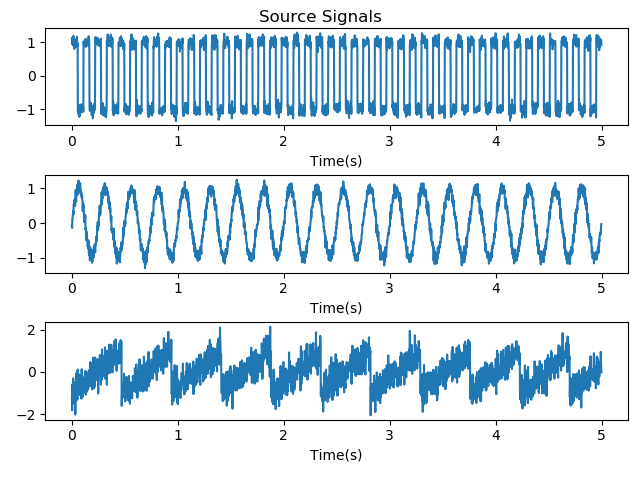
\includegraphics[width=\textwidth]{fwto/Signals_ica_1.png} \en
        \caption{} \gr
        \label{fig:5.1a}
    \end{subfigure}%
    \hfill
    \begin{subfigure}{0.48 \textwidth}
        \centering
       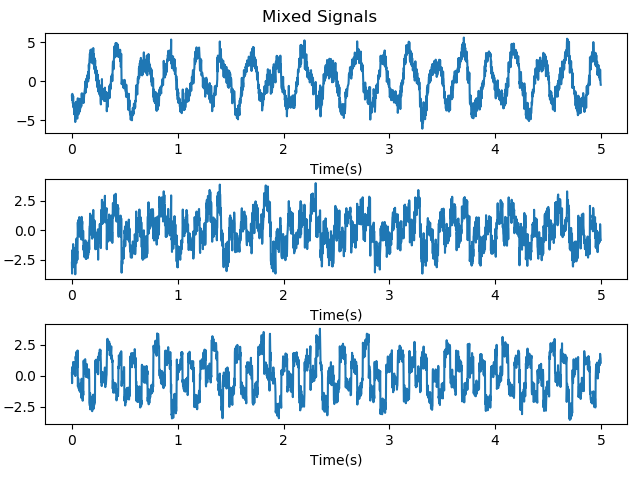
\includegraphics[width=\textwidth]{fwto/Mixed_ica_1.png}
        \en
        \caption{} \gr
        \label{fig:5.1b}
    \end{subfigure}%
    \gr
    \caption{Περιοδικές Πηγές και Μιξαρισμένα Σήματα}
\end{figure}
\noindent Τα σχήματα \en \ref{fig:5.2a} \gr και \en \ref{fig:5.2b} \gr είναι οι ανεξάρτητες συνιστώσες που εξάγει ο αλγόριθμος \en FastICA \gr για \en 'logcosh' \gr, τα σχήματα \en \ref{fig:5.3a} \gr   και \en \ref{fig:5.3b} \gr  για \en 'exp' \gr και τα σχήματα \en \ref{fig:5.4a} \gr και \en \ref{fig:5.4b} \gr για \en 'cube' \gr.
\begin{figure}[H]
    \centering
    \begin{subfigure}{0.48 \textwidth}
        \centering
        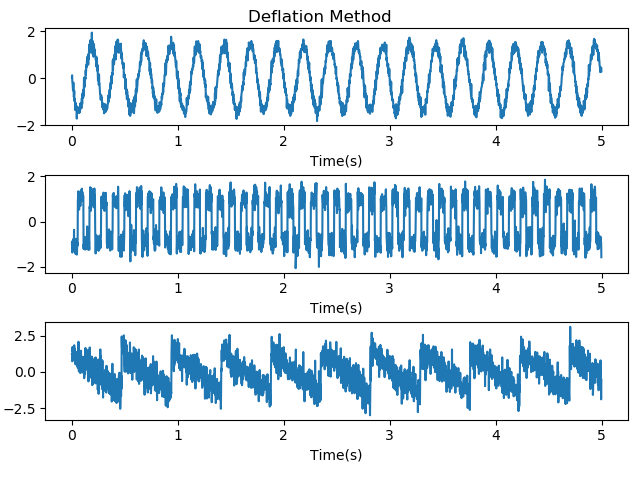
\includegraphics[width=\textwidth]{fwto/defla_ica_1_logcosh.png} \en
        \caption{Deflation} \gr
        \label{fig:5.2a}
    \end{subfigure}%
    \hfill
    \begin{subfigure}{0.48 \textwidth}
        \centering
    `   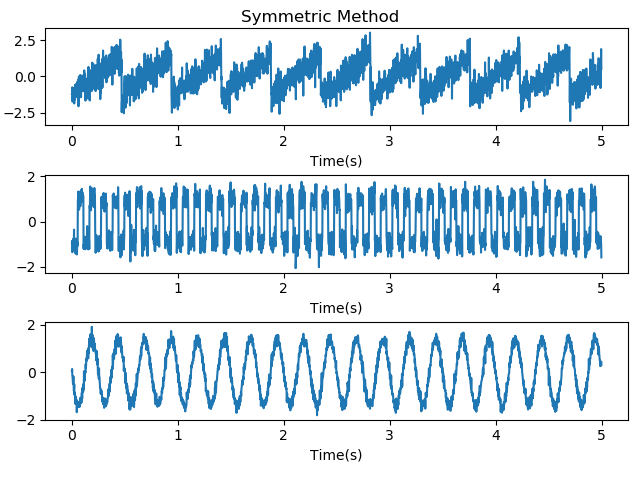
\includegraphics[width=\textwidth]{fwto/Symmetric_ica_1_logcosh.png}
        \en
        \caption{Symmetric} \gr
        \label{fig:5.2b}
    \end{subfigure}%
    \gr
    \caption{Ανεξάρτητες Συνιστώσες περιοδικών σημάτων για \en g = 'logcosh' \gr}
\end{figure}
\begin{figure}[H]
    \centering
    \begin{subfigure}{0.48 \textwidth}
        \centering
       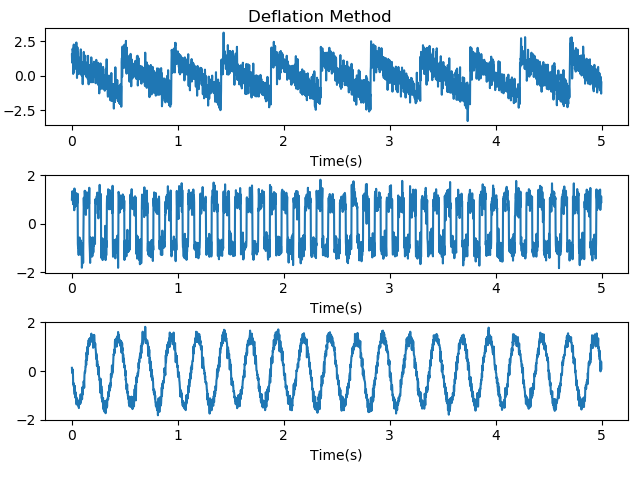
\includegraphics[width=\textwidth]{fwto/defla_ica_1_exp.png} \en
        \caption{Deflation} \gr
        \label{fig:5.3a}
    \end{subfigure}%
    \hfill
    \begin{subfigure}{0.48 \textwidth}
        \centering
       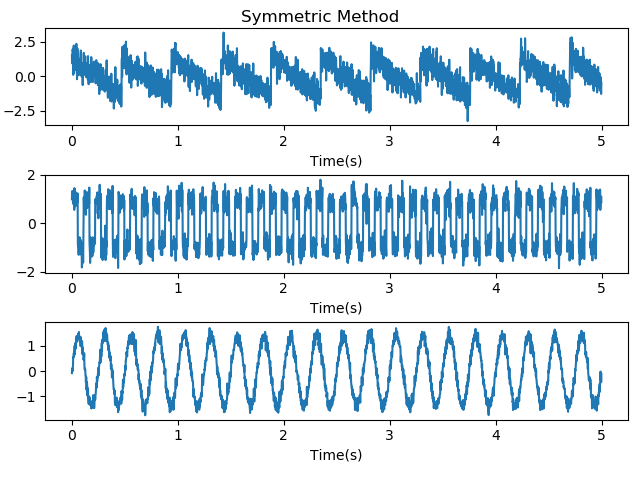
\includegraphics[width=\textwidth]{fwto/Symmetric_ica_1_exp.png}
        \en
        \caption{Symmetric} \gr
        \label{fig:5.3b}
    \end{subfigure}%
    \gr
    \caption{Ανεξάρτητες Συνιστώσες περιοδικών σημάτων για \en g = 'exp' \gr}
\end{figure}
\begin{figure}[H]
    \centering
    \begin{subfigure}{0.48 \textwidth}
        \centering
       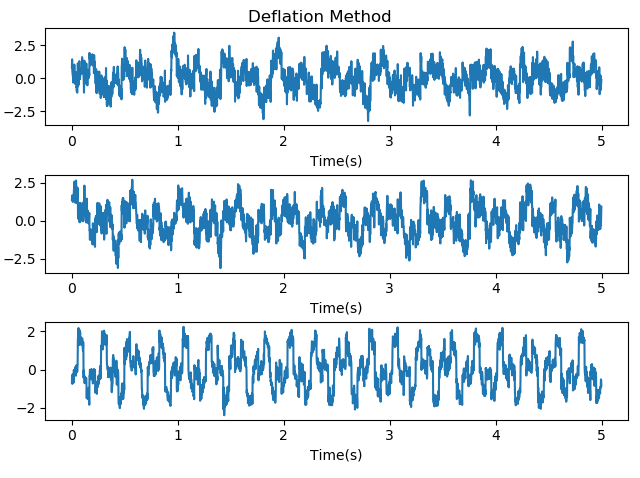
\includegraphics[width=\textwidth]{fwto/Deflation_ica_1_cube.png}\en
        \caption{Deflation} \gr
        \label{fig:5.4a}
    \end{subfigure}%
    %\hfill
    \begin{subfigure}{0.48 \textwidth}
        \centering
       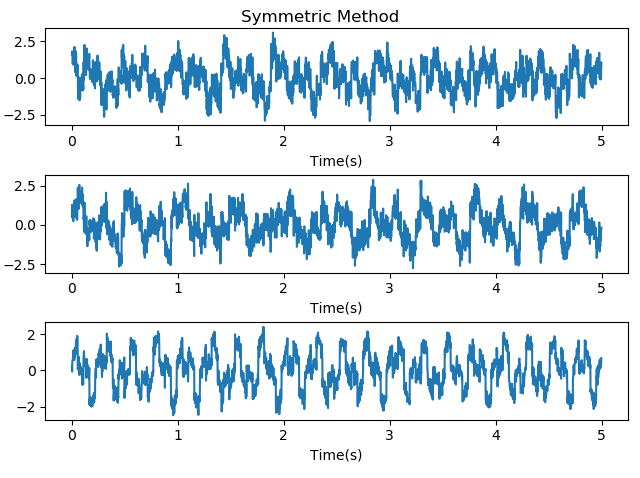
\includegraphics[width=\textwidth]{fwto/Symmetric_ica_1_cube.png}
        \en
        \caption{Symmetric} \gr
        \label{fig:5.4b}
    \end{subfigure}%
    \gr
    \caption{Ανεξάρτητες Συνιστώσες περιοδικών σημάτων για \en g = 'cube' \gr}
\end{figure}
\noindent Στα σχήματα \en \ref{fig:5.5a} \gr και \en \ref{fig:5.5b} \gr φαίνονται οι περιοδικές συνιστώσες που εξάγουν οι αλγόριθμοι π\en CA \gr και \en AMUSE \gr, ενώ στα σχήματα \en \ref{fig:5.6a} \gr και \en \ref{fig:5.6b} \gr τα αντίστοιχα περιοδικά σφάλματα.
\begin{figure}[H]
    \centering
    \begin{subfigure}{0.48 \textwidth}
        \centering
       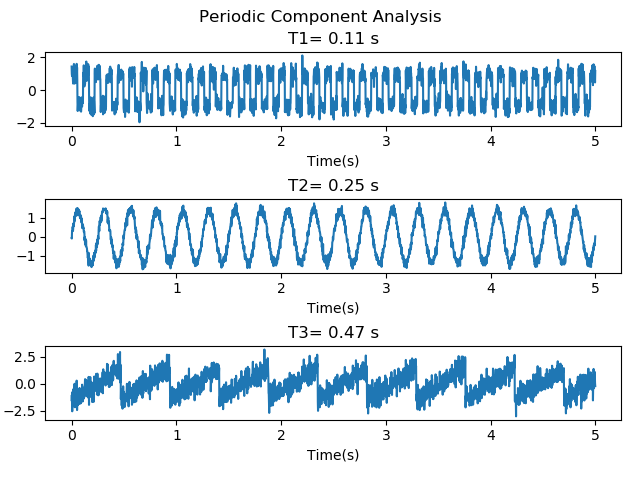
\includegraphics[width=\textwidth]{fwto/piCA_1.png}\en
        \caption{\gr Κανονική \en \pi CA} \gr
        \label{fig:5.5a}
    \end{subfigure}
    \hfill
    \begin{subfigure}{0.48 \textwidth}
        \centering
       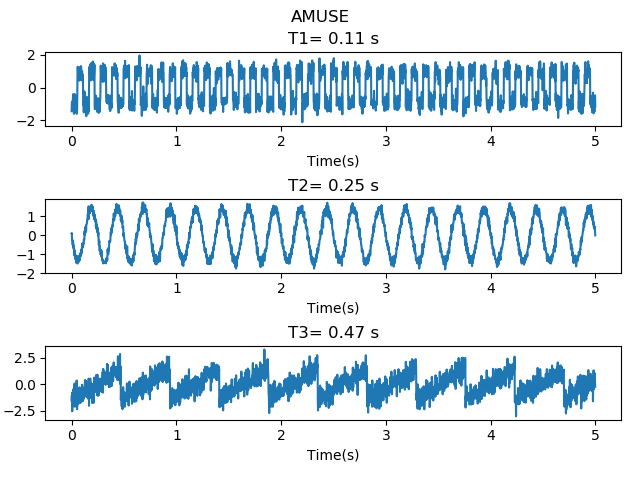
\includegraphics[width=\textwidth]{fwto/Amuse_1.png}
        \en
        \caption{AMUSE} \gr
        \label{fig:5.5b}
    \end{subfigure}
    \gr
    \caption{Εξαγωγή Περιοδικών Συνιστωσών για \en $T_1 = 0.11$ s, $T_2 = 0.25$ s \gr και \en $T_3 = 0.47$ s \gr}
\end{figure}
\begin{figure}[H]
    \centering
    \begin{subfigure}{0.48 \textwidth}
        \centering
       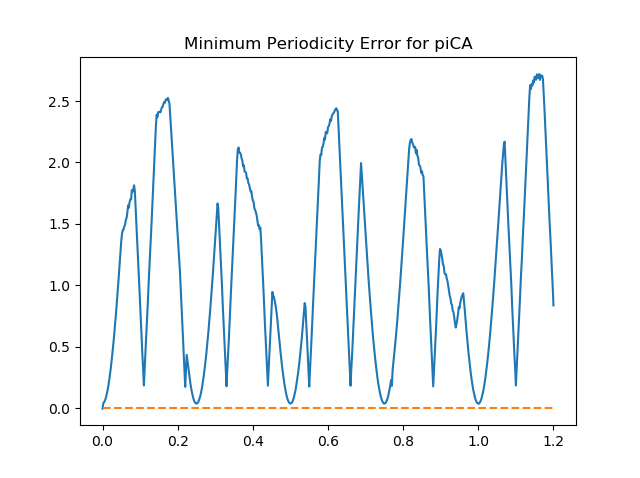
\includegraphics[width=\textwidth]{fwto/piCA_Error_1.png}\en
        \caption{\gr Κανονική \en \pi CA} \gr
        \label{fig:5.6a}
    \end{subfigure}
    \hfill
    \begin{subfigure}{0.48 \textwidth}
        \centering
       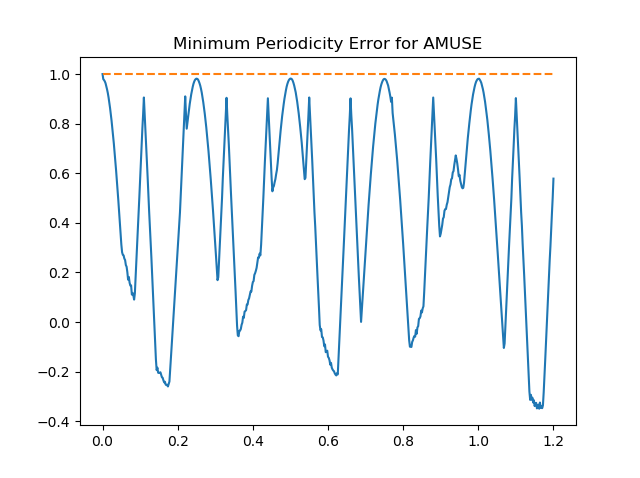
\includegraphics[width=\textwidth]{fwto/Amuse_Error_1.png}
        \en
        \caption{AMUSE} \gr
        \label{fig:5.6b}
    \end{subfigure}
    \gr
    \caption{Τα ελάχιστα σφάλματα για χρονική καθυστέρηση από 0 έως 1.2 δευτερόλεπτα}
\end{figure}
\noindent Τέλος, οι συντελεστές απόδοσης που υπολογίζονται από την \eqref{eq:5.1.1} φαίνονται παρακάτω: \en
\begin{table}[H] 
\centering
\begin{tabular}{|c|c|l|} 
\hline
          & Deflational  & Symmetric  \\ \hline
'logcosh' & 0.000847636 &  0.000818582 \\ \hline
'exp'     & 0.000951913 &  0.000261241 \\ \hline
'cube'    & 0.630938755 &  0.663469048 \\ \hline
πCA       & \multicolumn{2}{c|}{6.16798765e-05} \\ \hline
AMUSE     & \multicolumn{2}{c|}{6.16798765e-05} \\ \hline
\end{tabular}
\gr
\caption{Κριτήριο απόδοσης για κάθε υλοποιήσιμη μέθοδο}
\label{table:5.1}
\end{table}
\noindent Όπως βλέπουμε από τις γραφικές παραστάσεις, παρατηρούμε ότι, παρόλο της παρουσίας προσθετικού θορύβου, και η μέθοδος \en FastICA \gr αλλά και η π\en CA \gr αναγνωρίζουν πλήρως τα σήματα, εκτός της περίπτωσης \en 'cube' \gr της \en FastICA \gr . Από τον πίνακα απόδοσης \ref{table:5.1}, παρατηρούμε ότι σχεδόν όλοι οι αλγόριθμοι έχουν τιμή περίπου ίση με το 0, άρα προσεγγίζουν έναν πίνακα αντιμετάθεσης και επίσης, οι αλγόριθμοι που υποθέτουν περιοδικότητα έχουν αμυδρά καλύτερα αποτελέσματα κάτι που είναι προφανές εφόσον τα σήματα πηγών που χρησιμοποιήσαμε είναι περιοδικά.
\subsection{Ψευδό-Περιοδικά Σήματα}
\justifying
Θεωρούμε ως σήματα πηγών τα σήματα που φαίνονται στο σχήμα \ref{fig:5.7a}.
Βλέπουμε ότι τα δυο πρώτα σήματα αποτελούν συνδυασμούς σημάτων τα οποία έχουν επαναληφθεί στο πεδίο του χρόνου, κάνοντας τα ψευδό-περιοδικά ενώ το τελευταίο σήμα αποτελείται από 'λευκό' θόρυβο. Επιπλέον, για τα περιοδικά σήματα, οι περίοδοι επιλέχθηκαν αρχικά ως \en $T_1 = 0.5$ s \gr και \en $T_2 = 0.754$ s \gr και μεταβάλλουμε των αριθμό δειγμάτων τους κατά $a , b \in [-100 , 100]$ αντίστοιχα, οπότε δεν γνωρίζουμε την εκάστοτε περίοδο ακριβώς.
\\
Η διάρκεια των σημάτων είναι 5 δευτερόλεπτα ενώ η συχνότητα δειγματοληψίας είναι \en $f_s = 1 KHz$.\gr 
\\
Ο πίνακας μίξης είναι: \en
\begin{align*}
    \mathbf{A} = \begin{bmatrix}
    0.00740553 &  1.05634461 & -0.52022631 \\
    -0.00531442 &  0.95287344 & -0.26333002 \\
    -2.39713001 & -0.52477855 & -0.67513928 
    \end{bmatrix} \quad det(\mathbf{A}) = -0.5325
\end{align*}
\gr 
Τα σήματα πηγών και τα πεπλεγμένα σήματα φαίνονται στις εικόνες \en \ref{fig:5.7a} \gr και \en \ref{fig:5.7b} \gr.
\begin{figure}[H]
    \centering
    \begin{subfigure}{0.48 \textwidth}
        \centering
       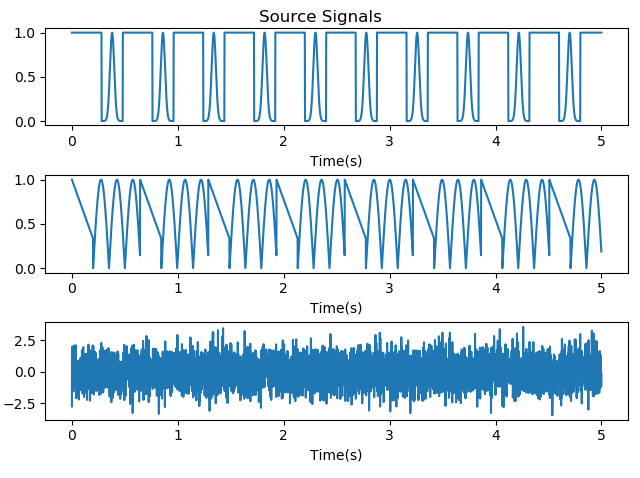
\includegraphics[width=\textwidth]{fwto/source.png} \en
        \caption{} \gr
        \label{fig:5.7a}
    \end{subfigure}
    \hfill
    \begin{subfigure}{0.48 \textwidth}
        \centering
       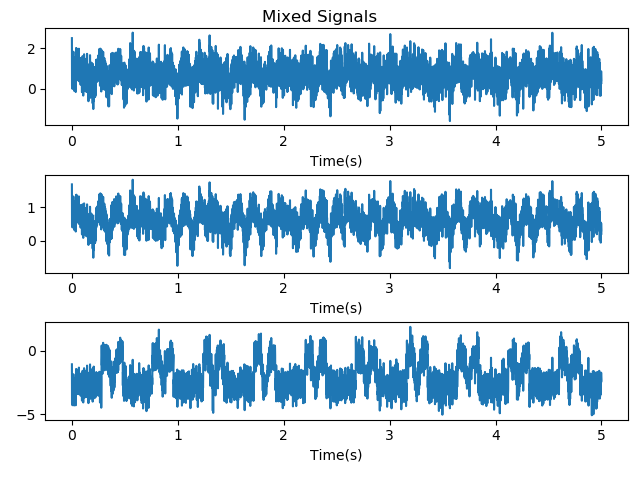
\includegraphics[width=\textwidth]{fwto/mixed.png}
        \en
        \caption{} \gr
        \label{fig:5.7b}
    \end{subfigure}
    \gr
    \caption{Ψευδο-περιοδικές Πηγές και Μιξαρισμένα Σήματα}
\end{figure}
\noindent Τα σχήματα \en \ref{fig:5.8a} \gr και \en \ref{fig:5.8b} \gr είναι οι ανεξάρτητες συνιστώσες που εξάγει ο αλγόριθμος \en FastICA \gr για \en 'logcosh' \gr, τα σχήματα \en \ref{fig:5.9a} \gr   και \en \ref{fig:5.9b} \gr  για \en 'exp' \gr και τα σχήματα \en \ref{fig:5.10a} \gr και \en \ref{fig:5.10b} \gr για \en 'cube' \gr.
\begin{figure}[H]
    \centering
    \begin{subfigure}{0.48 \textwidth}
        \centering
       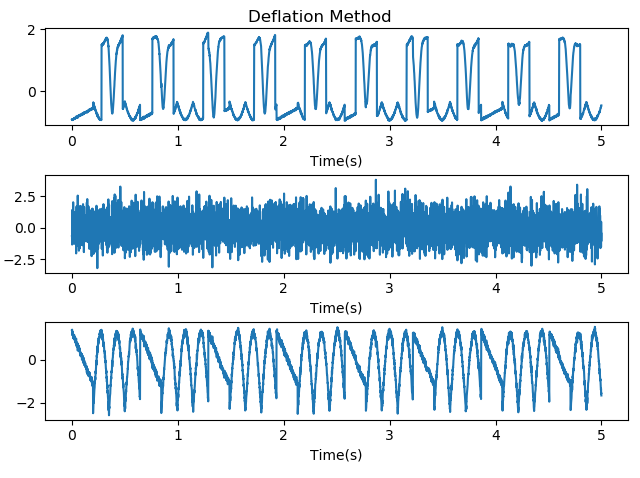
\includegraphics[width=\textwidth]{fwto/logcosh_def.png} \en
        \caption{Deflation} \gr
        \label{fig:5.8a}
    \end{subfigure}
    \hfill
    \begin{subfigure}{0.48 \textwidth}
        \centering
       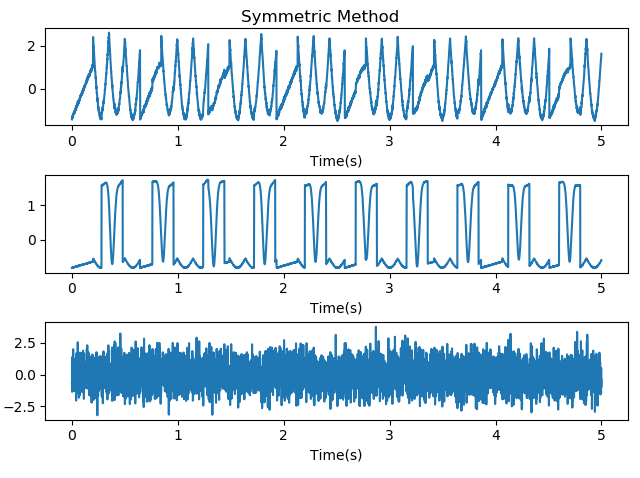
\includegraphics[width=\textwidth]{fwto/logcosh_sym.png} \en
        \en
        \caption{Symmetric} \gr
        \label{fig:5.8b}
    \end{subfigure}
    \gr
    \caption{Ανεξάρτητες Συνιστώσες περιοδικών σημάτων για \en g = 'logcosh' \gr}
\end{figure}
\begin{figure}[H]
    \centering
    \begin{subfigure}{0.48 \textwidth}
        \centering
       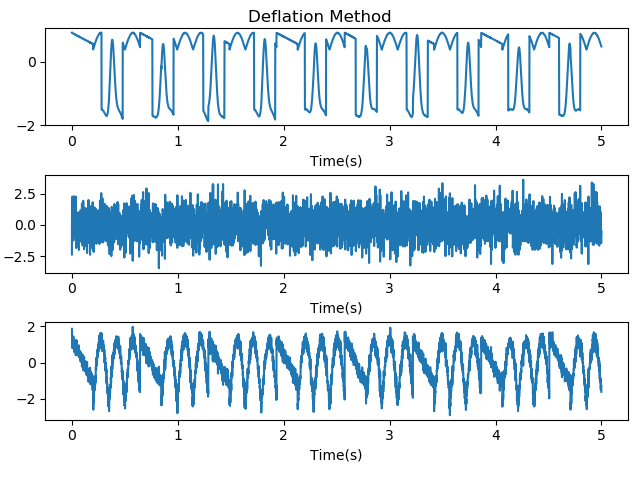
\includegraphics[width=\textwidth]{fwto/exp_def.png} \en
        \caption{Deflation} \gr
        \label{fig:5.9a}
    \end{subfigure}
    \hfill
    \begin{subfigure}{0.48 \textwidth}
        \centering
       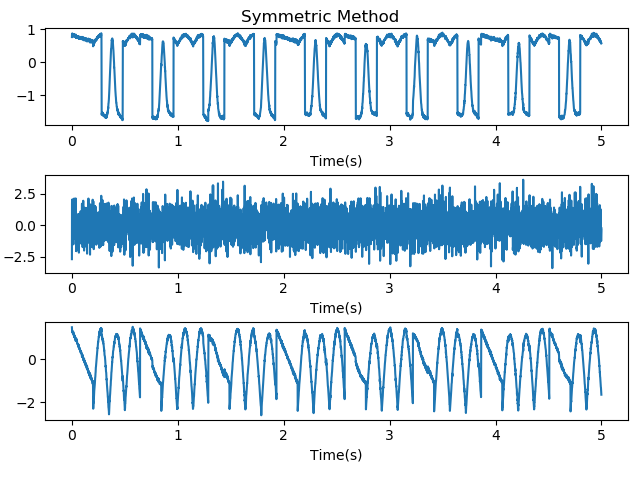
\includegraphics[width=\textwidth]{fwto/exp_sym.png}
        \en
        \caption{Symmetric} \gr
        \label{fig:5.9b}
    \end{subfigure}
    \gr
    \caption{Ανεξάρτητες Συνιστώσες περιοδικών σημάτων για \en g = 'exp' \gr}
\end{figure}
\begin{figure}[H]
    \centering
    \begin{subfigure}{0.48 \textwidth}
        \centering
       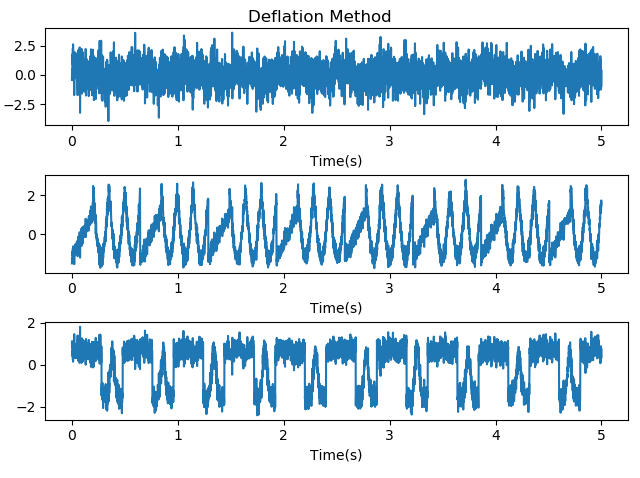
\includegraphics[width=\textwidth]{fwto/cube_def.png}\en
        \caption{Deflation} \gr
        \label{fig:5.10a}
    \end{subfigure}
    \hfill
    \begin{subfigure}{0.48 \textwidth}
        \centering
       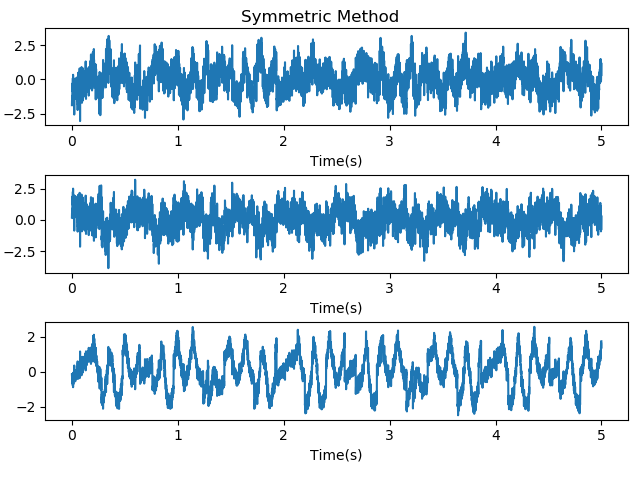
\includegraphics[width=\textwidth]{fwto/cube_sym.png}
        \en
        \caption{Symmetric} \gr
        \label{fig:5.10b}
    \end{subfigure}
    \gr
    \caption{Ανεξάρτητες Συνιστώσες περιοδικών σημάτων για \en g = 'cube' \gr}
\end{figure}
% fix ref
\noindent Στα σχήματα \en \ref{fig:5.11a} \gr και \en \ref{fig:5.11b} \gr φαίνονται οι περιοδικές συνιστώσες που εξάγουν οι αλγόριθμοι π\en CA \gr και \en AMUSE \gr, ενώ στα σχήματα \en \ref{fig:5.12a} \gr και \en \ref{fig:5.12b} \gr τα αντίστοιχα περιοδικά σφάλματα.
\en
\begin{figure}[H]
    \centering
    \begin{subfigure}{0.48 \textwidth}
        \centering
       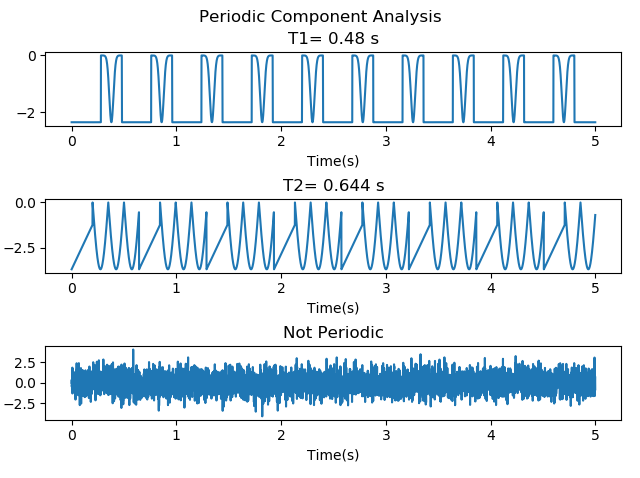
\includegraphics[width=\textwidth]{fwto/pica.png}\en
        \caption{\gr Κανονική \en \pi CA} \gr
        \label{fig:5.11a}
    \end{subfigure}
    \hfill
    \begin{subfigure}{0.48 \textwidth}
        \centering
       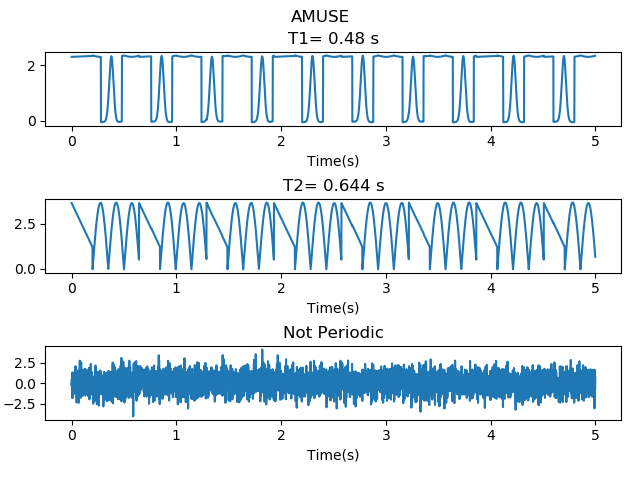
\includegraphics[width=\textwidth]{fwto/amuse.png}
        \en
        \caption{AMUSE} \gr
        \label{fig:5.11b}
    \end{subfigure}
    \gr
    \caption{Εξαγωγή Περιοδικών Συνιστωσών για \en $T_1 = 0.48$ s \gr και \en $T_2 = 0.644$ s \gr}
\end{figure}
\begin{figure}[H]
    \centering
    \begin{subfigure}{0.48 \textwidth}
        \centering
       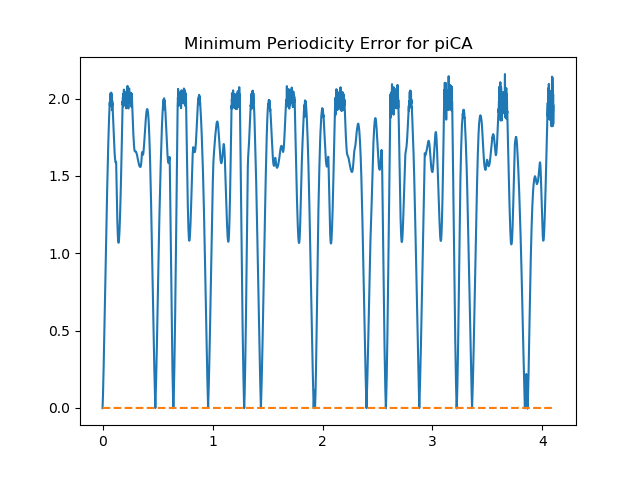
\includegraphics[width=\textwidth]{fwto/pica_error.png}\en
        \caption{\gr Κανονική \en \pi CA} \gr
        \label{fig:5.12a}
    \end{subfigure}
    \hfill
    \begin{subfigure}{0.48 \textwidth}
        \centering
       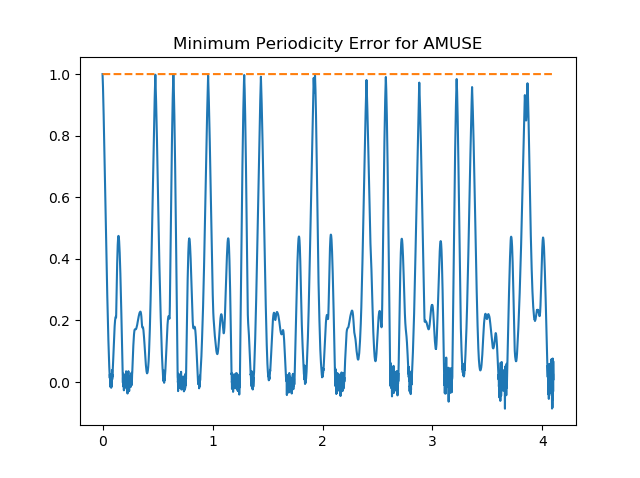
\includegraphics[width=\textwidth]{fwto/Amuse_Error.png}
        \en
        \caption{AMUSE} \gr
        \label{fig:5.12b}
    \end{subfigure}
    \gr
    \caption{Τα ελάχιστα σφάλματα για χρονική καθυστέρηση από 0 έως 4.2 δευτερόλεπτα}
\end{figure}
\noindent Τέλος, οι συντελεστές απόδοσης που υπολογίζονται από την \eqref{eq:5.1.1} φαίνονται παρακάτω: \en
\begin{table}[H] 
\centering
\begin{tabular}{|c|c|l|} 
\hline
          & Deflational  & Symmetric  \\ \hline
'logcosh' & 0.021798705 &  0.009850027 \\ \hline
'exp'     & 0.048388267 &  0.009237661 \\ \hline
'cube'    & 0.703621639 &  0.575454093 \\ \hline
πCA       & \multicolumn{2}{c|}{0.0005443894} \\ \hline
AMUSE     & \multicolumn{2}{c|}{0.0005443894} \\ \hline
\end{tabular}
\gr
\caption{Κριτήριο απόδοσης για κάθε υλοποιήσιμη μέθοδο}
\label{table:5.2}
\end{table}
\newpage
\noindent Παρατηρούμε ότι ο αλγόριθμος \en FastICA \gr και στις 3 περιπτώσεις, δεν εξάγει τα διάφορα σήματα επακριβώς αλλά εποπτικά, καθώς προσθέτει θόρυβο σε συνιστώσες που δεν είχαν, αντίθετα με τους αλγορίθμους π\en CA \gr και \en AMUSE \gr . Αυτό μπορεί να οφείλεται στο γεγονός ότι τα δεδομένα μας είναι αφιλτράριστα καθώς μπορεί να εμπεριέχονται συχνότητες στα δεδομένα μας που να δημιουργούν μια συσχέτιση με τον "λευκό" θόρυβο, κάνοντας τα μη-ανεξαρτήτα.
\section{Βιοσήματα}
\justifying
\iffalse
Κριτήριο αξιολόγησης μάλλον SNR na koitaxw papers
\fi
\subsection{Τεχνητά Βιοσήματα}
\justifying
Τα παρακάτω σήματα περιέχουν και πραγματικές και συνθετικές κυματομορφές, οι οποίες χρησιμοποιούνται για έλεγχο σε συσκευές που εποπτεύονται ηλεκτροκαρδιογραφήματα τα οποία λάβαμε από το \en Physionet ATM \gr \cite{signals:18} σε μορφή \en .txt \gr μέσω του πακέτου \en WFDB \gr \cite{db:19} από το \en Cygwin. \gr Επιλέγουμε 3 από τα διαθέσιμα σήματα, συγκεκριμένα τα \en "aami3a", "aami3b", \gr και \en "aami4a" \gr στα οποία δεν γνωρίζουμε την περίοδο τους. Καλούμαστε να αναγνωρίσουμε τα περιοδικά σημάτα, όπως και την περίοδο του καθενός, εκτελώντας τους αλγορίθμους με είσοδο των πίνακα που δημιουργείται από τα παραπάνω αρχεία. Το κάθε σήμα έχει διάρκεια 10 δευτερολέπτων και ρυθμό δειγματοληψίας ίσο με 720 \en Hz \gr, ανάλυση 12 \en bits \gr και τα πλάτος του κάθε σήματος είναι σε \en mV \gr. 
\\ [0.5 \baselineskip]
Τα σήματα πηγής φαίνονται στο σχήμα \ref{fig:5.13}:
\begin{figure}[H]
    \centering
    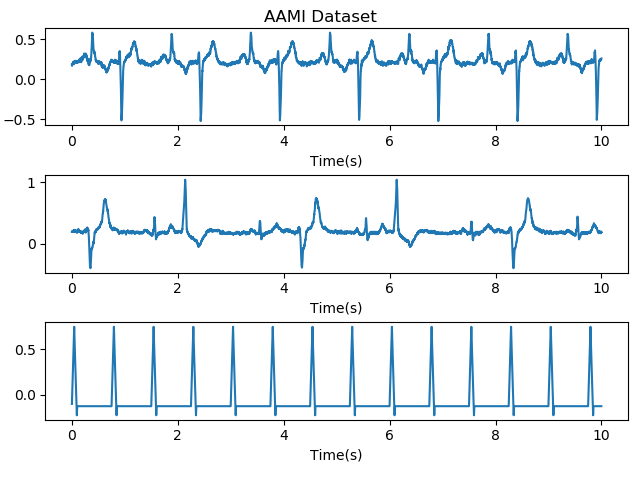
\includegraphics[width=\textwidth]{biosignals/aami_source.png}
    \caption{\en AAMI Dataset} \gr
    \label{fig:5.13}
\end{figure}
\noindent Τα σχήματα \en \ref{fig:5.14a} \gr και \en \ref{fig:5.14a} \gr είναι οι ανεξάρτητες συνιστώσες που εξάγει ο αλγόριθμος \en FastICA \gr για \en 'logcosh' \gr, τα σχήματα \en \ref{fig:5.15a} \gr   και \en \ref{fig:5.15b} \gr  για \en 'exp' \gr και τα σχήματα \en \ref{fig:5.16a} \gr και \en \ref{fig:5.16b} \gr για \en 'cube' \gr.
\begin{figure}[H]
    \centering
    \begin{subfigure}{0.48 \textwidth}
        \centering
       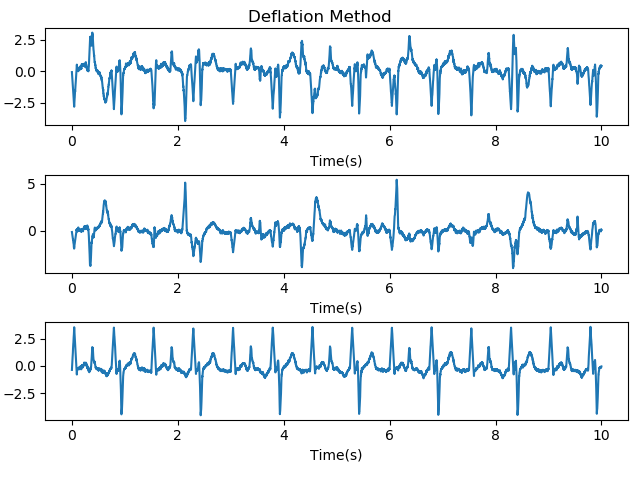
\includegraphics[width=\textwidth]{biosignals/aami_logcosh_def.png} \en
        \caption{Deflation} \gr
        \label{fig:5.14a}
    \end{subfigure}
    \hfill
    \begin{subfigure}{0.48 \textwidth}
        \centering
       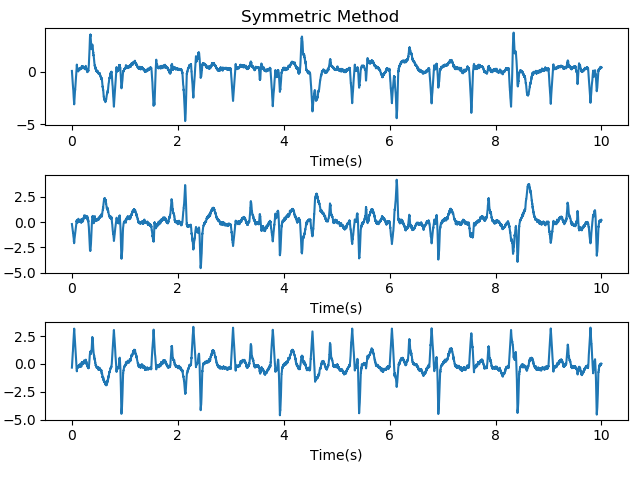
\includegraphics[width=\textwidth]{biosignals/aami_logcosh_sym.png} \en
        \en
        \caption{Symmetric} \gr
        \label{fig:5.14b}
    \end{subfigure}
    \gr
    \caption{Αποτελέσματα για \en g = 'logcosh' \gr}
\end{figure}
\begin{figure}[H]
    \centering
    \begin{subfigure}{0.48 \textwidth}
        \centering
       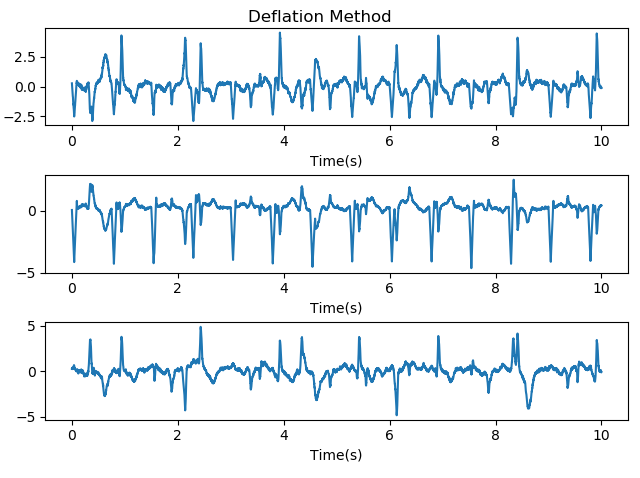
\includegraphics[width=\textwidth]{biosignals/aami_exp_def.png} \en
        \caption{Deflation} \gr
        \label{fig:5.15a}
    \end{subfigure}
    \hfill
    \begin{subfigure}{0.48 \textwidth}
        \centering
       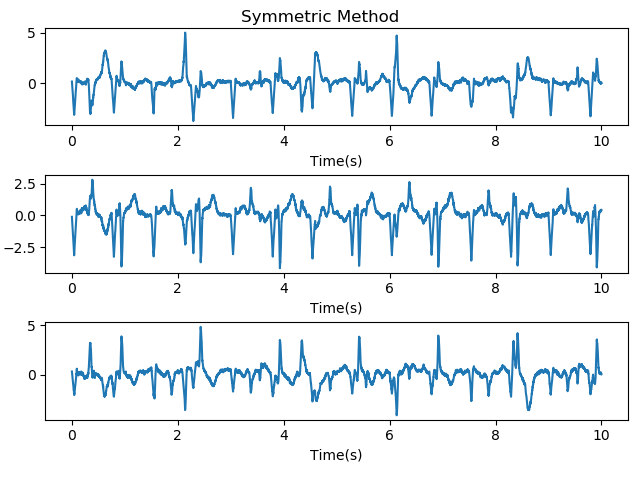
\includegraphics[width=\textwidth]{biosignals/aami_exp_sym.png} \en
        \en
        \caption{Symmetric} \gr
        \label{fig:5.15b}
    \end{subfigure}
    \gr
    \caption{Αποτελέσματα για \en g = 'exp' \gr}
\end{figure}
\begin{figure}[H]
    \centering
    \begin{subfigure}{0.48 \textwidth}
        \centering
       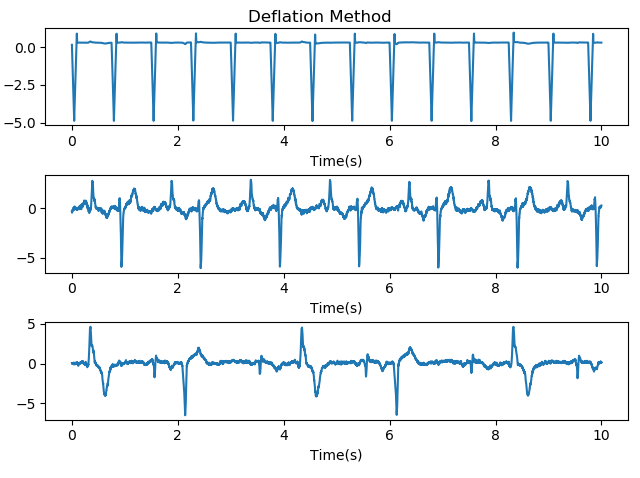
\includegraphics[width=\textwidth]{biosignals/aami_cube_def.png} \en
        \caption{Deflation} \gr
        \label{fig:5.16a}
    \end{subfigure}
    \hfill
    \begin{subfigure}{0.48 \textwidth}
        \centering
       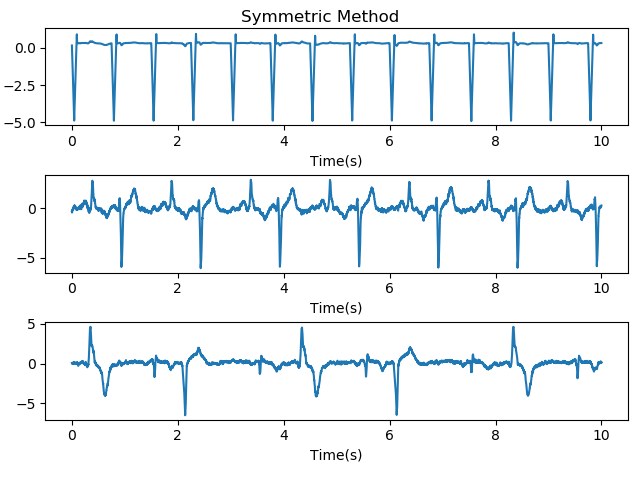
\includegraphics[width=\textwidth]{biosignals/aami_cube_sym.png} \en
        \en
        \caption{Symmetric} \gr
        \label{fig:5.16b}
    \end{subfigure}
    \gr
    \caption{Αποτελέσματα για \en g = 'cube' \gr}
\end{figure}
\noindent Στα σχήματα \en \ref{fig:5.17a} , \ref{fig:5.17b} \gr
φαίνονται οι περιοδικές συνιστώσες με τις αντίστοιχες περιόδους και στα σχήματα \en \ref{fig:5.18a}, \ref{fig:5.18b} \gr
τα αντίστοιχα περιοδικά σφάλματα.
\begin{figure}[H]
    \centering
    \begin{subfigure}{0.48 \textwidth}
        \centering
       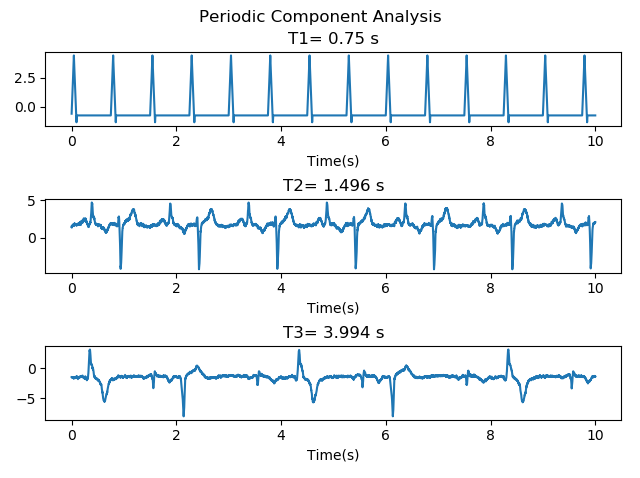
\includegraphics[width=\textwidth]{biosignals/aami_pica.png}\en
        \caption{\gr Κανονική \en \pi CA} \gr
        \label{fig:5.17a}
    \end{subfigure}
    \hfill
    \begin{subfigure}{0.48 \textwidth}
        \centering
       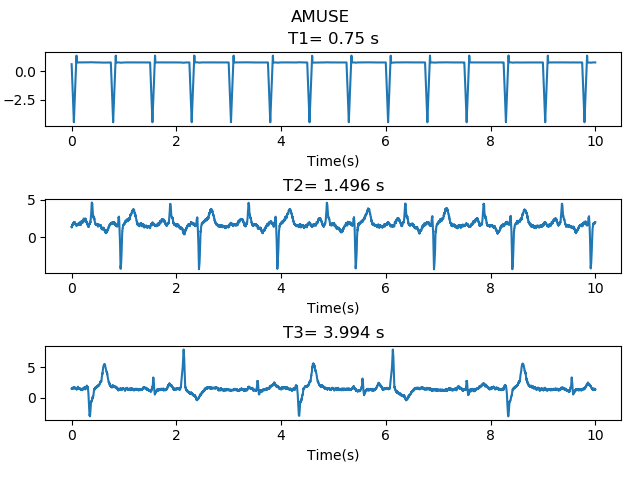
\includegraphics[width=\textwidth]{biosignals/aami_amuse.png}
        \en
        \caption{AMUSE} \gr
        \label{fig:5.17b}
    \end{subfigure}
    \gr
    \caption{Οι περιοδικές συνιστώσες του \en AAMI Dataset \gr για \en $T_1 = 0.75$ s, $T_2 = 1.496$ s \gr και \en $T_3 = 3.994$ s \gr }
\end{figure}
\begin{figure}[H]
    \centering
    \begin{subfigure}[b]{0.48 \textwidth}
        \centering
       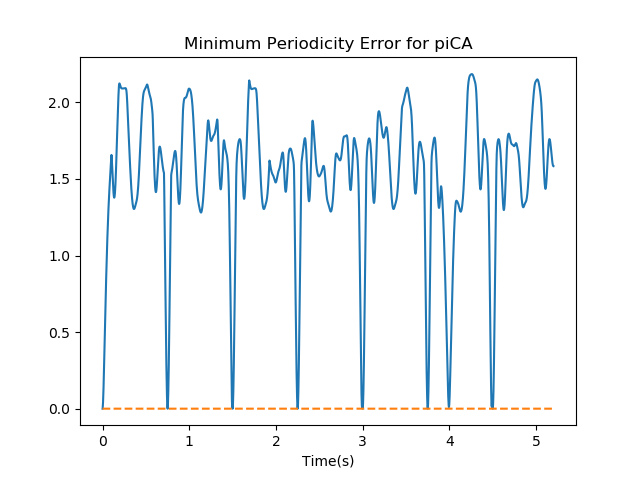
\includegraphics[width=\textwidth]{biosignals/aami_pica_error.png}\en
        \caption{\gr Κανονική \en \pi CA} \gr
        \label{fig:5.18a}
    \end{subfigure}
    \hfill
    \begin{subfigure}[b]{0.48 \textwidth}
        \centering
       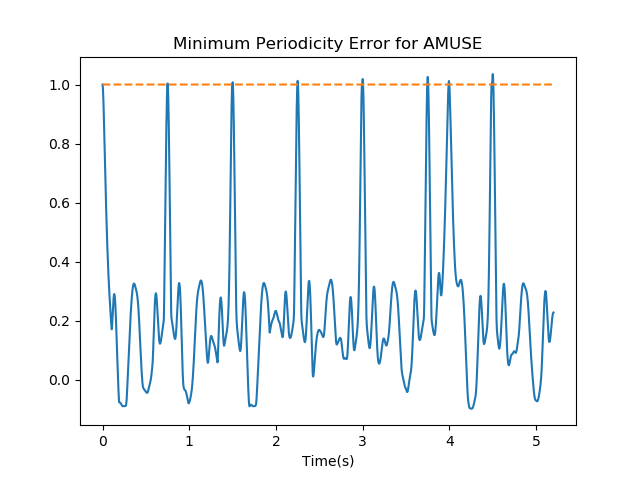
\includegraphics[width=\textwidth]{biosignals/aami_amuse_error.png}
        \en
        \caption{AMUSE} \gr
        \label{fig:5.18b}
    \end{subfigure}
    \gr
    \caption{Τα ελάχιστα περιοδικά σφάλματα για χρονική καθυστέρηση από 0 έως 5.2 δευτερόλεπτα}
\end{figure}
\noindent Βλέπουμε ότι ο αλγόριθμος π\en CA \gr βγάζει καθαρά τα σήματα όπως περιμέναμε, αναγνωρίζοντας και την περίοδο του καθενός. 'Οσο για τον αλγόριθμο \en Fast ICA, \gr στην περίπτωση \en 'cube' \gr λαμβάνουμε αρκετά καλά αποτελέσματα, δηλαδή μικρή αλλοίωση την τελική μορφή των σημάτων, και στις δυο προσεγγίσεις ενώ οι άλλες δύο περιπτώσεις αποτυγχάνουν πλήρως στην αναγνώριση των αρχικών σημάτων.  
\subsection{Πραγματικά Βιοσήματα - Παράδειγμα 1}
\justifying
Η βάση δεδομένων που θα χρησιμοποιήσουμε είναι η \en "Abdominal and Direct Fetal Electrocardiogram Database (adfecgdb)" \gr 
\cite{examples:20}\cite{examples:21}\cite{examples:22}
και συγκεκριμένα θα χρησιμοποιήσουμε τα σήματα \en r01.edf, \gr που κατεβάσαμε και αποθηκεύσαμε σε αρχείο \en .txt \gr μέσω του πακέτου \en WFDB \gr.
\\[0.5 \baselineskip]
Τα δεδομένα περιέχουν πολυκάναλες καταγραφές εμβρυακών ηλεκτροκαρδιογραφημάτων από 5 γυναίκες μεταξύ 38 και 41 εβδομάδων κύησης. Κάθε καταγραφή περιλαμβάνει 4 διαφορικά σήματα που αποκτήθηκαν από την κοιλία της μητέρας και 1 εμβρυακό ηλεκτροκαρδιογράφημα ως σήμα αναφοράς, από το κεφάλι του εμβρύου. Το εύρος ζώνης των σημάτων είναι \en 1 Hz - 150 Hz \gr και έχει φιλτραριστεί η παρεμβολή των \en 50 Hz \gr από την παροχή ρεύματος, όπως και οι χαμηλές συχνότητες του \en baseline drift \gr που οφείλονται στην κίνηση και την αναπνοή του μητέρας. Επιπλέον, όλα τα σήματα έχουν δειγματοληφθεί ταυτόχρονα με ρυθμό δειγματοληψίας \en $F_s = 1 kHz$ \gr με ακρίβεια 16 \en bits \gr και τα πλάτη των όλων των σημάτων είναι σε \en mV. \gr
\\ [0.5 \baselineskip]
Θα προσπαθήσουμε να εξάγουμε το μητρικό και το εμβρυακό \en ECG \gr με τις παραπάνω μεθόδους. Θα χρησιμοποιήσουμε το εμβρυακό ηλεκτροκαρδιογράφημα ως σήμα αναφοράς για την σύγκριση των εξαχθέντων συνιστωσών και τα υπόλοιπα ως μικτά σήματα προς εξαγωγή των συνιστωσών. Για την σύγκριση των σημάτων με το εμβρυακό \en ECG, \gr θα υπολογίσουμε τις θέσεις των \en RR-intervals, \gr δηλαδή της χρονικής διαφοράς μεταξύ \en R peaks \gr  από το σήμα αναφοράς. Σε όποια σήματα συμπίπτουν τα παραπάνω σημεία, θα αποτελούν εμβρυακά ενώ οποιοδήποτε περιοδικό σήμα, διάφορο του σήματος αναφοράς, θα αποτελεί μητρικό σήμα.
\\ [1.5 \baselineskip]
Στο σχήμα \ref{fig:5.19} φαίνονται τα πρώτα 12 δευτερόλεπτα του αρχείου \en r01 \gr και στο σχήμα \ref{fig:5.20} φαίνονται οι θέσεις των \en RR peaks \gr του εμβρυακού ηλεκτροκαρδιογραφήματος
\begin{figure}[H]
    \centering
    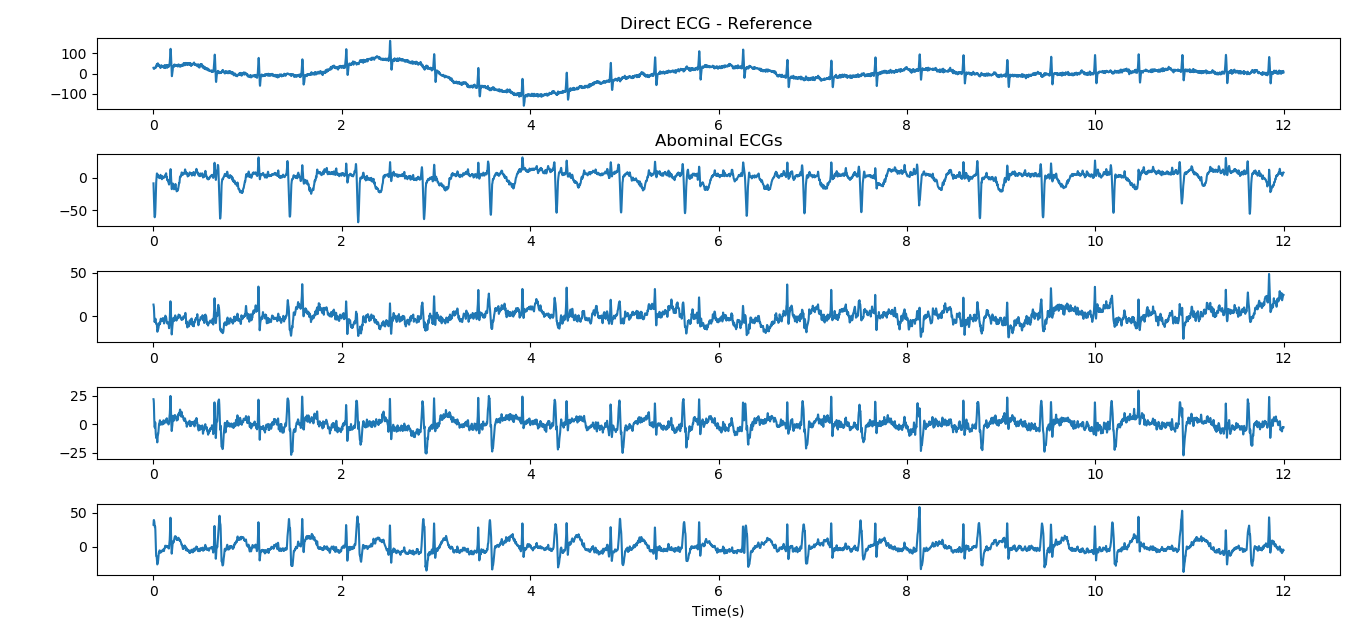
\includegraphics[width=\textwidth]{r01database/r01_12secs.png}
    \caption{Σήματα Ηλεκτροδίων της \en r01 \gr}
    \label{fig:5.19}
\end{figure}
\begin{figure}[H]
    \centering
    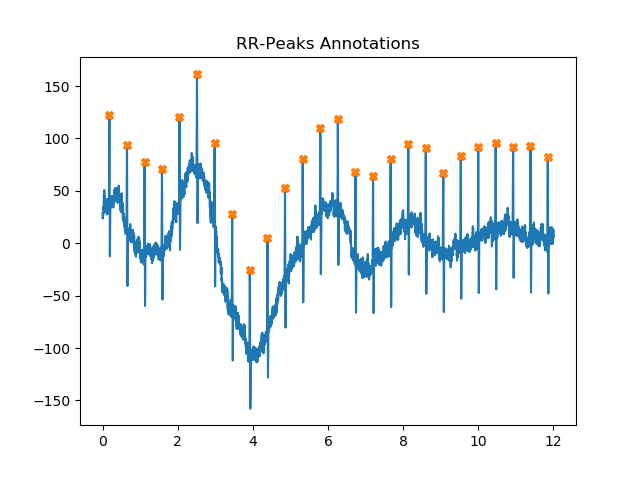
\includegraphics[width=0.7 \textwidth]{r01database/RR_peaks_annotations.png}
    \caption{Τα \en RR intervals \gr του εμβρυακού \en ECG \gr}
    \label{fig:5.20}
\end{figure}
\noindent Στα σχήματα \en \ref{fig:5.21a} \gr και \en \ref{fig:5.21b} \gr φαίνονται οι ανεξάρτητες συνιστώσες για \en 'logcosh'. \gr Στο πρώτο σχήμα, μπορούμε να πούμε ότι η 3η συνιστώσα αποτελεί το εμβρυακό και η 4η το μητρικό ενώ στο δεύτερο σχήμα, το 1ο είναι το εμβρυακό και το 4ο το μητρικό. Η Συμμετρική προσέγγιση βλέπουμε ότι αναγνωρίζει καλύτερα το εμβρυακό σήμα ενώ για το μητρικό δεν μπορούμε να αποφανθούμε περαιτέρω.
\begin{figure}[H]
    \centering
    \begin{subfigure}{0.48 \textwidth}
        \centering
       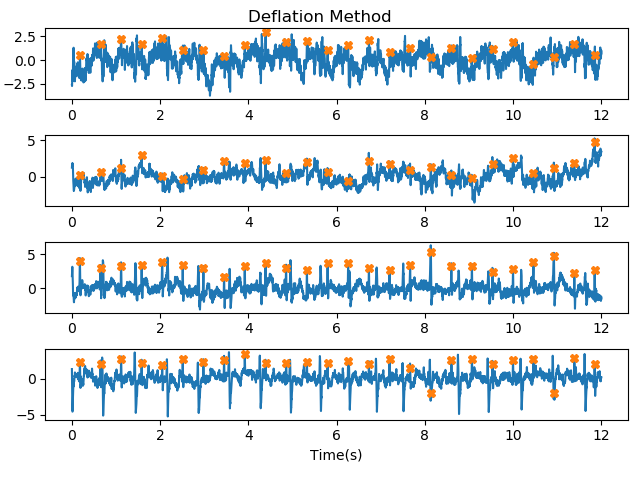
\includegraphics[width=\textwidth]{r01database/logcosh_def.png} \en
        \caption{Deflation} \gr
        \label{fig:5.21a}
    \end{subfigure}
    \hfill
    \begin{subfigure}{0.48 \textwidth}
        \centering
       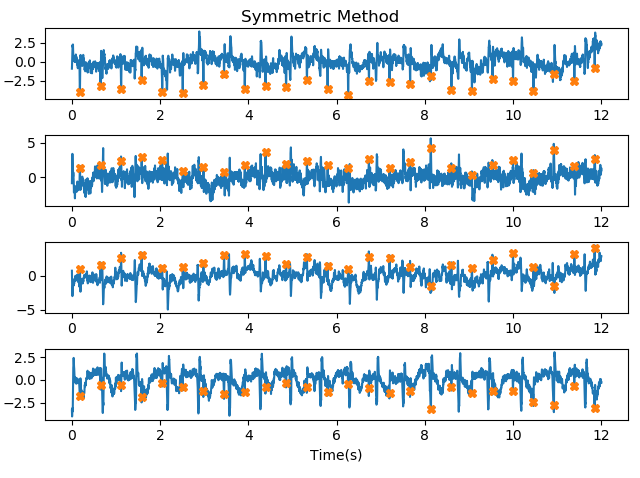
\includegraphics[width=\textwidth]{r01database/logcosh_sym.png} \en
        \en
        \caption{Symmetric} \gr
        \label{fig:5.21b}
    \end{subfigure}
    \gr
    \caption{Αποτελέσματα για \en g = 'logcosh' \gr}
\end{figure}
%%
\noindent Στα σχήματα \en \ref{fig:5.22a} \gr και \en \ref{fig:5.22b} \gr φαίνονται οι ανεξάρτητες συνιστώσες για \en 'exp'. \gr Στο πρώτο σχήμα, η 4η συνιστώσα είναι πιο κοντά στο εμβρυακό \en ECG \gr ενώ στπ δεύτερο σχήμα, το 1ο είναι το εμβρυακό και το 4ο το μητρικό. Όπως και στην \en 'logcosh' \gr περίπτωση, βλέπουμε ότι η Συμμετρική προσέγγιση παράγει καλύτερα αποτελέσματα.
\begin{figure}[H]
    \centering
    \begin{subfigure}{0.48 \textwidth}
        \centering
       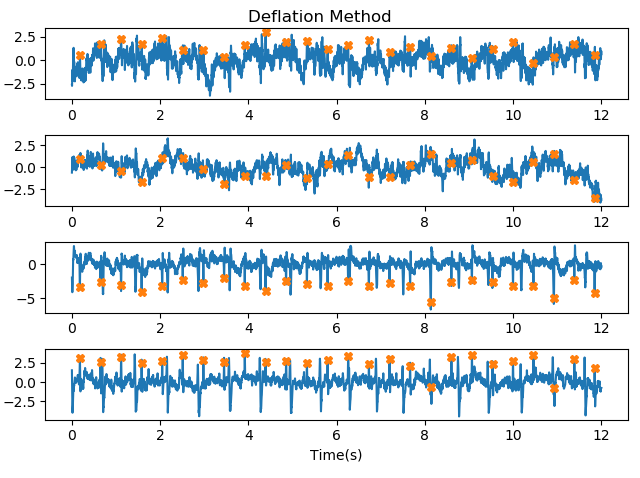
\includegraphics[width=\textwidth]{r01database/exp_def.png} \en
        \caption{Deflation} \gr
        \label{fig:5.22a}
    \end{subfigure}
    \hfill
    \begin{subfigure}{0.48 \textwidth}
        \centering
       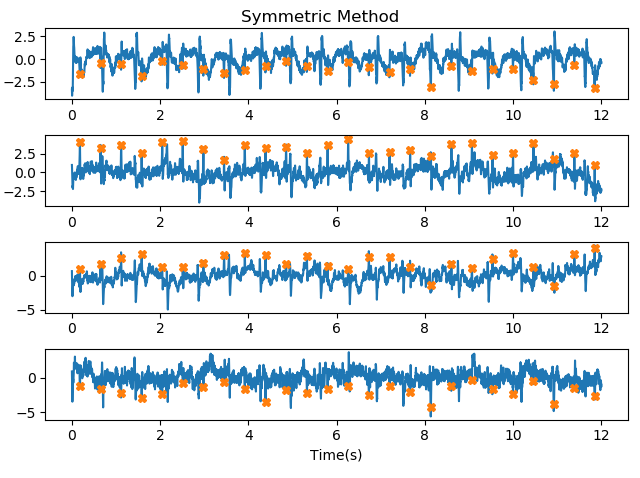
\includegraphics[width=\textwidth]{r01database/exp_sym.png} \en
        \en
        \caption{Symmetric} \gr
        \label{fig:5.22b}
    \end{subfigure}
    \gr
    \caption{Αποτελέσματα για \en g = 'exp' \gr}
\end{figure}
\noindent Στα σχήματα \en \ref{fig:5.23a} \gr και \en \ref{fig:5.23b} \gr φαίνονται οι ανεξάρτητες συνιστώσες για \en 'cube'. \gr Στο πρώτο σχήμα, η 1η συνιστώσα είναι το εμβρυακό \en ECG \gr και το 2ο το μητρικό ενώ στο δεύτερο σχήμα, το 4ο είναι το εμβρυακό και το 2ο το μητρικό. Σε αντίθεση με τις άλλες συναρτήσεις, η συνάρτηση \en 'cube' \gr εξάγει καλά αποτελέσματα και στις δύο περιπτώσεις.
\begin{figure}[H]
    \centering
    \begin{subfigure}{0.48 \textwidth}
        \centering
       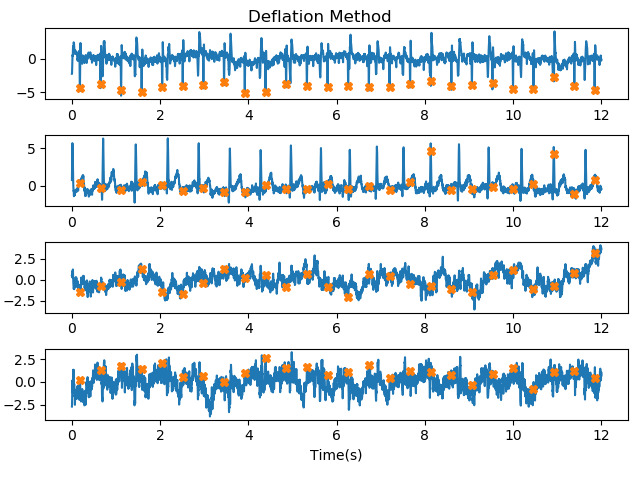
\includegraphics[width=\textwidth]{r01database/cube_def.png} \en
        \caption{Deflation} \gr
        \label{fig:5.23a}
    \end{subfigure}
    \hfill
    \begin{subfigure}{0.48 \textwidth}
        \centering
       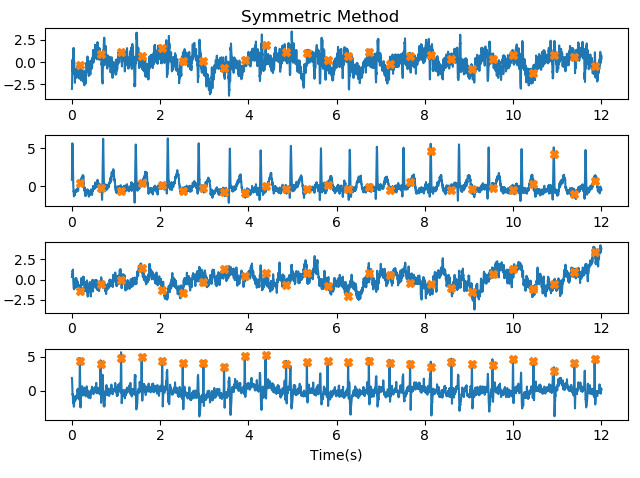
\includegraphics[width=\textwidth]{r01database/cube_sym.png} \en
        \en
        \caption{Symmetric} \gr
        \label{fig:5.23b}
    \end{subfigure}
    \gr
    \caption{Αποτελέσματα για \en g = 'cube' \gr}
\end{figure}
%
\noindent Στο σχήμα \ref{fig:5.24} φαίνονται οι περιοδικές συνιστώσες που εξάγονται από τον π\en CA. \gr Το πρώτο σχήμα δίνει ως πρώτη συνιστώσα το εμβρυακό \en ECG \gr και το δεύτερο σχήμα το μητρικό αντίστοιχα. Πρέπει να τονίσουμε ότι στο δεύτερο σχήμα, πήραμε ως αναφορά τα \en R peaks \en του μητρικού \en ECG \gr. Παρατηρούμε επίσης ότι η 3η συνιστώσα του πρώτου σχήματος και του δεύτερου σχήματος είναι το μητρικό και εμβρυακό \en ECG \gr αντίστοιχα.
\begin{figure}[H] 
    \centering
    \begin{subfigure}{0.48 \textwidth}
        \centering
        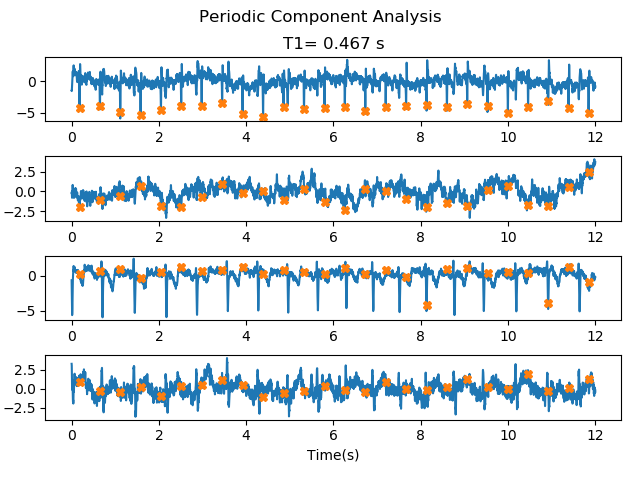
\includegraphics[width=\textwidth]{r01database/infant_pica.png}\en
    \end{subfigure}
    \hfill
    \begin{subfigure}{0.48 \textwidth}
        \centering
        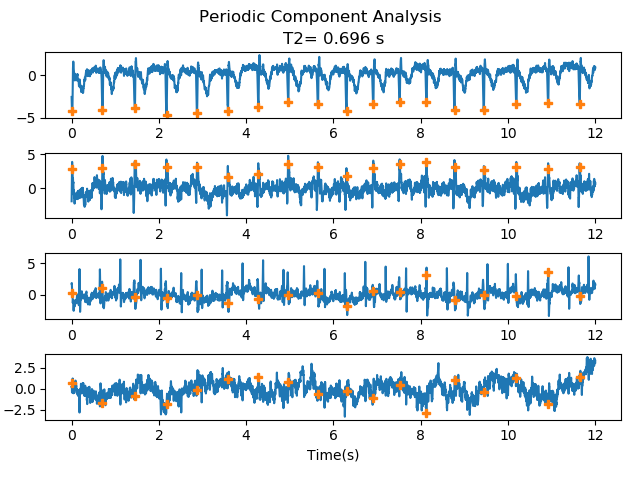
\includegraphics[width=\textwidth]{r01database/mother_pica.png}\en
    \end{subfigure}
    \gr
    \caption{Περιοδικές συνιστώσες για π\en CA \gr με περιόδους \en $Τ_1 = 0.467 s$ \gr και \en $Τ_2 = 0.696 s$ \gr  }
    \label{fig:5.24}
\end{figure} 
%
\noindent Στο σχήμα \ref{fig:5.25} φαίνονται οι περιοδικές συνιστώσες που εξάγονται μέσω \en AMUSE. \gr Παρατηρούμε τα ίδια ακριβώς αποτελέσματα με τον αλγόριθμο π\en CA. \gr
\begin{figure}[H] 
    \centering
    \begin{subfigure}{0.48 \textwidth}
        \centering
        \includegraphics[width=\textwidth]{r01database/amuse_infant.png}\en
    \end{subfigure}
    \hfill
    \begin{subfigure}{0.48 \textwidth}
        \centering
        \includegraphics[width=\textwidth]{r01database/amuse_mother.png}\en
    \end{subfigure}
    \gr
    \caption{Περιοδικές συνιστώσες για \en AMUSE \gr με περιόδους \en $Τ_1 = 0.467 s$ \gr και \en $Τ_2 = 0.696 s$ \gr  }
    \label{fig:5.25}
\end{figure} 
\noindent Τέλος, στο σχήμα φαίνονται τα περιοδικά σφάλματα για τους αλγόριθμους π\en CA \gr και \en AMUSE. \gr
\begin{figure}[H]
    \centering
    \begin{subfigure}[b]{0.48 \textwidth}
        \centering
       \includegraphics[width=\textwidth]{r01database/pica_error.png}\en
        \caption{\gr Κανονική \en \pi CA} \gr
    \end{subfigure}
    \hfill
    \begin{subfigure}[b]{0.48 \textwidth}
        \centering
        \includegraphics[width=\textwidth]{r01database/amuse_error.png}\en
        \caption{AMUSE} \gr
    \end{subfigure}
    \gr
    \caption{Τα ελάχιστα περιοδικά σφάλματα για χρονική καθυστέρηση από 0 έως 1.6 δευτερόλεπτα}
    \label{fig:5.26}
\end{figure}
\subsection{Πραγματικά Βιοσήματα - Περίπτωση 2}
\justifying
Η βάση δεδομένων που θα χρησιμοποιήσουμε είναι η \en DaISy \gr \cite{daisy:24} που περιέχει πολυκάναλες καταγραφές του δερματικού δυναμικού μιας εγκύου γυναίκας. Τα δεδομένα περιέχουν 5 καταγραφές γύρω από την κοιλιακή κοιλότητα της μητέρας και 3 θωρακικές καταγραφές που φαίνονται στο σχήμα \ref{fig:5.27}. Τα σήματα έχουν δειγματοληφθεί ταυτόχρονα με ρυθμό δειγματοληψίας 250 \en Hz \gr, έχουν διάρκεια 10 δευτερολέπτων και το πλάτος τους είναι σε \en mV. \gr Τα σήματα είναι σε μορφή \en .dat \gr με πρώτη στήλη τα δείγματα σε μορφή δευτερολέπτων ενώ οι υπόλοιπες στήλες τις παρατηρήσεις των ηλεκτροκαρδιογραφημάτων. 
% butterworth filtro
\newpage
\noindent Ο σκοπός μας είναι, όπως και στην προηγούμενη ενότητα, να αναγνωρίσουμε το εμβρυακό και το μητρικό \en ECG \gr με μόνη διαφορά ότι το σήμα αναφοράς θα είναι ένα από τα θωρακικά ηλεκτροκαρδιογραφήματα των δεδομένων, συγκεκριμένα το μητρικό \en ECG. \gr Άρα, οποιοδήποτε περιοδικό σήμα με διαφορετικά \en R peaks \gr θα είναι το εμβρυακό.
\begin{figure}[H]
    \centering
    \begin{subfigure}[b]{0.48 \textwidth}
        \centering
       \includegraphics[width=\textwidth]{daisy/Abdominals.png}\en
        \caption{\gr Κοιλιακά Ηλεκτροκαρδιογραφήματα} \gr
    \end{subfigure}
    \hfill
    \begin{subfigure}[b]{0.48 \textwidth}
        \centering
        \includegraphics[width=\textwidth]{daisy/Thoracic.png}\en
        \caption{\gr Θωρακικά Ηλεκτροκαρδιογραφήματα} \gr
    \end{subfigure}
    \gr
    \caption{Βάση δεδομένων \en DaISy \gr}
    \label{fig:5.27}
\end{figure}
\begin{figure}[H]
    \centering
    \includegraphics[width=0.7 \textwidth]{daisy/maternal_reference.png}
    \caption{Τα \en RR intervals \gr του μητρικού \en ECG \gr που λαμβάνονται από τον θώρακα}
    \label{fig:5.28}
\end{figure}
\noindent Αξίζει να σημειωθεί ότι η εφαρμογή φίλτρου δεν φέρει μεγάλο αποτέλεσμα,καθώς όπως φαίνεται και από το σχήμα \ref{fig:5.35}, το φάσμα των παρατηρήσεων είναι γύρω από τις συχνότητες \en 1 Hz  \gr έως \en 20Hz. \gr Οπότε καλούμαστε να εξάγουμε τις συνιστώσες ενδιαφέροντος υπό την παρουσία θορύβου.
\begin{figure}[H]
    \centering
    \includegraphics[width=0.7 \textwidth]{daisy/fft.png}
    \caption{Συχνοτικό φάσμα των παρατηρήσεων}
    \label{fig:5.35}
\end{figure}
\noindent Στα σχήματα \ref{fig:5.29a} και \ref{fig:5.29b} φαίνονται οι ανεξάρτητες συνιστώσες για \en 'logcosh' \gr. Παρατηρούμε ότι στην πρώτη εικόνα, τα σχήματα 7,8 αντιστοιχούν στο μητρικό \en ECG \gr ενώ το 6 θυμίζει το εμβρυακό, ενώ στην δεύτερη εικόνα δεν μπορούμε να βγάλουμε συμπεράσματα. 
\begin{figure}[H]
    \centering
    \begin{subfigure}{0.48 \textwidth}
        \centering
       \includegraphics[width=\textwidth]{daisy/logcosh_def.png} \en
        \caption{Deflation} \gr
        \label{fig:5.29a}
    \end{subfigure}
    \hfill
    \begin{subfigure}{0.48 \textwidth}
        \centering
       \includegraphics[width=\textwidth]{daisy/logcosh_sym.png} \en
        \en
        \caption{Symmetric} \gr
        \label{fig:5.29b}
    \end{subfigure}
    \gr
    \caption{Αποτελέσματα για \en g = 'logcosh' \gr}
\end{figure}
\noindent Στα σχήματα \ref{fig:5.30a} και \ref{fig:5.30b} φαίνονται οι ανεξάρτητες συνιστώσες για \en 'exp' \gr. Παρατηρούμε ότι στην πρώτη εικόνα, το σχήμα 8 αντιστοιχεί στο μητρικό \en ECG \gr χωρίς να έχουμε βρει το εμβρυακό ενώ στην δεύτερη εικόνα δεν μπορούμε πάλι να βγάλουμε συμπεράσματα. 
\begin{figure}[H]
    \centering
    \begin{subfigure}{0.48 \textwidth}
        \centering
       \includegraphics[width=\textwidth]{daisy/exp_def.png} \en
        \caption{Deflation} \gr
        \label{fig:5.30a}
    \end{subfigure}
    \hfill
    \begin{subfigure}{0.48 \textwidth}
        \centering
       \includegraphics[width=\textwidth]{daisy/exp_sym.png} \en
        \en
        \caption{Symmetric} \gr
        \label{fig:5.30b}
    \end{subfigure}
    \gr
    \caption{Αποτελέσματα για \en g = 'exp' \gr}
\end{figure}
\noindent Στα σχήματα \ref{fig:5.31a} και \ref{fig:5.31b} φαίνονται οι ανεξάρτητες συνιστώσες για \en 'cube' \gr. Παρατηρούμε ότι στην πρώτη εικόνα, τα σχήματα 1, 2 και 3 αντιστοιχούν στο μητρικό \en ECG \gr και το 4ο στο εμβρυακό, ενώ στην συμμετρική προσέγγιση, το 4ο σχήμα είναι το εμβρυακό και τα σχήματα 1, 3 και 5 το μητρικό. Βλέπουμε επιπλέον ότι ο αλγόριθμος \en FastICA \gr δίνει αρκετά καλά αποτελέσματα με την χρήση της συνάρτησης \en $x^3$ \gr.
\begin{figure}[H]
    \centering
    \begin{subfigure}{0.48 \textwidth}
        \centering
       \includegraphics[width=\textwidth]{daisy/cube_def.png} \en
        \caption{Deflation} \gr
        \label{fig:5.31a}
    \end{subfigure}
    \hfill
    \begin{subfigure}{0.48 \textwidth}
        \centering
       \includegraphics[width=\textwidth]{daisy/cube_sym.png} \en
        \en
        \caption{Symmetric} \gr
        \label{fig:5.31b}
    \end{subfigure}
    \gr
    \caption{Αποτελέσματα για \en g = 'cube' \gr}
\end{figure}
\noindent Στο σχήμα \ref{fig:5.32} φαίνονται οι περιοδικές συνιστώσες που εξάγονται από τον π\en CA. Η πρώτη γραφική παράσταση φανερώνει ως πρώτη συνιστώσα το εμβρυακό ηλεκτροκαρδιογράφημα με την αντίστοιχη περίοδο ενώ στο τέλος βλέπουμε το μητρικό. Αντίστοιχα, στην δεύτερη γραφική παράσταση, παρατηρούμε ότι το μητρικό ηλεκτροκαρδιογράφημα φαίνεται στην πρώτη θέση με την παρουσία θορύβου, όσο αφορά τα \en R peaks, \gr αλλά και στην πέμπτη καθαρότερα, ακολουθώντας τα εμβρυακά. Αυτό το γεγονός μάλλον οφείλεται στην παρουσία θορύβου, όπως αναφέραμε παραπάνω, αλλά κα στην ακρίβεια του βήματος που χρησιμοποιούμε ως \en timelag \gr.
\begin{figure}[H] 
    \centering
    \begin{subfigure}{0.48 \textwidth}
        \centering
        \includegraphics[width=\textwidth]{daisy/pica_infant.png}\en
    \end{subfigure}
    \hfill
    \begin{subfigure}{0.48 \textwidth}
        \centering
        \includegraphics[width=\textwidth]{daisy/pica_maternal.png}
        \en
    \end{subfigure}
    \gr
    \caption{Περιοδικές συνιστώσες για π\en CA \gr με περιόδους \en $Τ_1 = 0.448 s$ \gr και \en $Τ_2 = 0.74 s$ \gr  }
    \label{fig:5.32}
\end{figure} 
\noindent Αντίστοιχα, στο σχήμα \ref{fig:5.33} φαίνονται οι περιοδικές συνιστώσες που εξάγoνται από τον \en AMUSE. \gr Βλέπουμε τα ίδια ακριβώς ίδια αποτελέσματα με τον π\en CA \gr. 
\begin{figure}[H] 
    \centering
    \begin{subfigure}{0.48 \textwidth}
        \centering
        \includegraphics[width=\textwidth]{daisy/amuse_infant.png}\en
    \end{subfigure}
    \hfill
    \begin{subfigure}{0.48 \textwidth}
        \centering
        \includegraphics[width=\textwidth]{daisy/amuse_maternal.png}
        \en
    \end{subfigure}
    \gr
    \caption{Περιοδικές συνιστώσες για \en AMUSE \gr με περιόδους \en $Τ_1 = 0.448 s$ \gr και \en $Τ_2 = 0.74 s$ \gr  }
    \label{fig:5.33}
\end{figure} 
\noindent Τέλος, στο σχήμα \ref{fig:5.34} φαίνονται τα περιοδικά σφάλματα για τους παραπάνω αλγορίθμους.
\begin{figure}[H]
    \centering
    \begin{subfigure}[b]{0.48 \textwidth}
        \centering
       \includegraphics[width=\textwidth]{daisy/pica_error.png}\en
        \caption{\gr Κανονική \en \pi CA} \gr
    \end{subfigure}
    \hfill
    \begin{subfigure}[b]{0.48 \textwidth}
        \centering
        \includegraphics[width=\textwidth]{daisy/amuse_error.png}\en
        \caption{AMUSE} \gr
    \end{subfigure}
    \gr
    \caption{Τα ελάχιστα περιοδικά σφάλματα για χρονική καθυστέρηση από 0 έως 1.2 δευτερόλεπτα}
    \label{fig:5.34}
\end{figure}
\noindent Όπως και με τα προηγούμενα σήματα, βλέπουμε ότι οι αλγόριθμοι π\en CA \gr και \en AMUSE \gr αναγνωρίζουν αρκετά καλά τα σήματα ενδιαφέροντος, σε αντίθεση με τον αλγόριθμο \en FastICA. \gr
\subsection{Αξιολόγηση στην εξαγωγή βιοσημάτων}
\justifying
Για την αξιολόγηση των πραγματικών σημάτων \cite{criterion:25}, θα υπολογίσουμε την ακρίβεια - \en Accuracy \gr και την ευαισθησία - \en Sensivity \gr στα αποτελέσματα που λάβαμε από τον π\en CA \gr στα κεφάλαια 5.2.2 και 5.2.3 . Εφόσον με τον αλγόριθμο π\en CA \gr λαμβάνουμε την περιοδική συνιστώσα με ελάχιστο περιοδικό σφάλμα σε κάθε \en timelag, \gr αρκεί μόνο να εξετάσουμε την πρώτη συνιστώσα για κάθε περίοδο.
\\[0.5 \baselineskip]
Ως \en Sensivity \gr ορίζεται το ποσοστό των \en R peaks \gr που αναγνωρίστηκαν σωστά από τον αλγόριθμο και ως \en Accuracy \gr την συνολική ορθότητα της μεθόδου. Συγκεκριμένα:
\begin{align} \label{eq:5.2.1}
    Sensivity = \frac{TP}{TP+FN} 
\end{align}
\begin{align} \label{eq:5.2.2}
    Accuracy = \frac{TP}{TP+FN+FP}
\end{align}
όπου
\begin{itemize}
    \item \en TP (True Positive) \gr ο αριθμός των \en peak \gr του εκάστοτε σήματος αναφοράς
    \item \en FN (False Negative) \gr ο αριθμός των \en peak \gr που παρέλειψε να αναγνωρίσει ο αλγόριθμος
    \item \en FP (False Positive) \gr ο αριθμός των \en peak \gr που αναγνώρισε εσφαλμένα ο αλγόριθμος
\end{itemize}
Στους παρακάτω πίνακες φαίνονται τα ποσοστά των κριτηρίων των σχέσεων \eqref{eq:5.2.1} και \eqref{eq:5.2.2}:
\begin{table}[H] 
\centering
\begin{tabular}{|c|c|c|} 
\hline
          & \gr Εμβρυακό \en ECG  & \gr Μητρικό \en ECG  \\ \hline
\en Sensivity & 100 \% &  100 \% \\ \hline
\en Accuracy  & 100 \% &  100 \% \\ \hline
\end{tabular}
\gr
\caption{Απόδοση του \en abfecg dataset\gr }
\label{table:5.3}
\end{table}
\begin{table}[H] 
\centering
\begin{tabular}{|c|c|c|} 
\hline
          & \gr Εμβρυακό \en ECG  & \gr Μητρικό \en ECG  \\ \hline
\en Sensivity & 100 \% &  100 \% \\ \hline
\en Accuracy  & 100 \% &  87.5 \% \\ \hline
\end{tabular}
\gr
\caption{Απόδοση του \en DaISy dataset\gr }
\label{table:5.4}
\end{table}
\noindent Στo \en abfecgdb dataset \gr έχουμε 26 κορυφές για το εμβρυακό \en ECG \gr και 18 κορυφές για το μητρικό, με τον αλγόριθμο να τις αναγνωρίζει όλες. Απο την άλλη, στο \en DaISy dataset, \gr έχουμε 26 κορυφές για το εμβρυακό, που αναγνωρίζονται όλες και 14 για το μητρικό, εκ των οποίων οι 2 αναγνωρίζονται εσφαλμένα.

\chapter{\textbf{Συμπεράσματα και Μελλοντική Έρευνα}} \label{ch:ch6}
Με τα αποτελέσματα των αλγορίθμων που παρουσιάσαμε και εκτελέσαμε στην παρούσα εργασία για τεχνητά και πραγματικά σήματα, μπορούμε να καταλήξουμε στα ακόλουθα συμπεράσματα:
\begin{enumerate}
    \item Η υπόθεση ότι όλα τα σήματα έχουν περιοδική δομή, ιδιαίτερα όταν ασχολούμαστε με βιοσήματα, είναι ' ισχυρότερη ' από την υπόθεση ότι όλα τα επιμέρους σήματα είναι ανεξάρτητα. Για αυτόν τον λόγο, ο αλγόριθμος π\en CA \gr υπερισχύει του αλγορίθμου \en FastICA \gr στην εξαγωγή συνιστωσών με περιοδική δομή.
    \item Ο αλγόριθμος π\en CA \gr είναι πιο αποδοτικός από άποψη χρόνου, καθώς απαιτείται μόνο ο υπολογισμός 3 πινάκων σε αντίθεση με τον επαναληπτικό αλγόριθμο σύγκλισης του \en FastICA. \gr
    \item Στον αλγόριθμο \en ICA \gr δεν είναι δυνατόν να προβλέψουμε την σειρά των εξαγώμενων συνιστωσών σε αντίθεση με τον π\en CA, \gr όπου οι εξαγώμενες συνιστώσες ταξινομούνται με βάση την περιοδικότητα τους.
    \item Οι ιδιοτιμές που υπολογίζονται από την σχέση \eqref{eq:4.1.10} αποτελούν ένα μέτρο της ύπαρξης θορύβου στις εξαγώμενες συνιστώσες και μπορούν να χρησιμοποιηθούν ως κατώφλι για την απόρριψη ασήμαντων συνιστωσών. Με άλλα λόγια, εάν θεωρήσουμε κάθε απεριοδικό σήμα πηγής ως θόρυβο, η μέθοδος π\en CA \gr μπορεί να ερμηνευτεί ως μετασχηματισμός που κατανέμει την διασπορά του θορύβου στις λιγότερο σημαντικές συνιστώσες. Με τον αλγόριθμο \en FastICA \gr δεν μπορεί να επιτευχθεί αυτό καθώς αναζητεί τις πιο ανεξάρτητες και όχι τις πιο περιοδικές (λιγότερο θορυβώδεις) συνιστώσες.
\end{enumerate}
\newpage
\noindent Τέλος, μερικές προτάσεις για μελλοντική έρευνα είναι:
\begin{itemize}
    \item η εύρεση μεθόδου συγχρονισμού των σημείων ενδιαφέροντος ώστε να μην υπάρχουν αλλαγές στην φάση των εξαγόμενων περιοδικών συνιστωσών και παρουσιάζονται ανεστραμμένες.
    \item η δημιουργία γραφικής διεπαφής (\en GUI) \gr για την εύρεση και την αναπαράσταση περιοδικών συνιστωσών.
    \item η ανάπτυξη μεθόδων εύρεσης βέλτιστου βήματος για την χρονική καθυστέρηση με σκοπό τον βέλτιστο συνδυασμό ακρίβειας και ταχύτητας.
    \item η δυνατότητα επέκτασης των μεθόδων για πιο περίπλοκα συστήματα \en BSS. \gr
    \item η εφαρμογή και σύγκριση των μεθόδων που παρουσιάστηκαν σε αυτή την εργασία και σε άλλα περιοδικά σήματα.
\end{itemize}
\appendix
\chapter{Κώδικες}
Οι κώδικες είναι \en Python \gr με χρήση των βιβλιοθηκών \en NumPy\cite{python:30}, SciPy\cite{python:29} \gr και \en matplotlib\cite{python:31}. \gr Γράφτηκαν στο \en Spyder IDE \gr και υλοποιήθηκαν με την έκδοση 3.6.5
\en
\section{\en fastica.py}
\en
\inputminted[linenos,fontsize=\scriptsize]{python}{codes/fastica.py}
\newpage
\section{\en deflational method.py}
\en
\inputminted[linenos,fontsize=\scriptsize]{python}{codes/deflational_method.py}
\newpage
\section{\en symmetric method.py}
\en
\inputminted[linenos,fontsize=\scriptsize]{python}{codes/symmetric_method.py}
\newpage
\section{\en piCA.py}
\en
\inputminted[linenos,fontsize=\scriptsize]{python}{codes/piCA.py}
\newpage
\section{\en preproc.py}
\en
\inputminted[linenos,fontsize=\scriptsize]{python}{codes/preproc.py}
\newpage
\section{\en is def.py}
\en
\inputminted[linenos,fontsize=\scriptsize]{python}{codes/misc.py}
\newpage
\section{\en C0/Ct.py}
\en
\inputminted[linenos,fontsize=\scriptsize]{python}{codes/C0_Ct.py}
\newpage
\section{\en Ce.py}
\en
\inputminted[linenos,fontsize=\scriptsize]{python}{codes/C_e.py}
\newpage
\section{\en Rayleigh Minimum.py}
\en
\inputminted[linenos,fontsize=\scriptsize]{python}{codes/rayleigh_minimum.py}
\newpage
\section{\en min/max.py}
\en
\inputminted[linenos,fontsize=\scriptsize]{python}{codes/min_max.py}
\newpage
\section{\en period check correlation.py}
\en
\inputminted[linenos,fontsize=\scriptsize]{python}{codes/period_check_correlation.py}
\en
\bibliography{bibliography}
\bibliographystyle{ieeetr}

\end{document}





